\documentclass[table, t,13pt]{beamer} 
\usepackage{graphicx}
\usepackage{xeCJK,fontspec,xunicode,xltxtra, beamerthemesplit, fancybox}

%box tools
\usepackage{framed, color}
\definecolor{shadecolor}{rgb}{1, 0.8, 0.3}


% 以下为表格颜色和线条控制的package
\usepackage[]{xcolor} %xcolor宏包提供的命令\rowcolors,注意需要宏包的table选项支持,即:
%如上命令可以使表格带上背景色,它的语法是:
%\rowcolors [<commands>]{<row>}{<odd-row color >}{<even-row color >}
\rowcolors{1}{white}{blue!5}

\usepackage{colortbl} %细粒度控制表格的颜色
\definecolor{rowheadcolor}{rgb}{0.9, 0.9, 0.9} %定义表格标题行的颜色

\usepackage{makecell} % 控制线宽

\usetheme[height=8mm]{Madrid} % My favorite! 
%\usetheme[height=10mm]{Rochester}
%\usetheme[height=10mm]{Boadilla} % Pretty neat, soft color. 
%\usetheme{default} 
%\usetheme{Warsaw} 
%\usetheme{Bergen} % This template has nagivation on the left 
%\usetheme{Frankfurt} % Similar to the default 

% 以下设置页面底部的信息
\makeatletter
\setbeamertemplate{footline}
{
  \leavevmode%
  \hbox{%
  \begin{beamercolorbox}[wd=.333333\paperwidth,ht=2.25ex,dp=1ex,center]{author in head/foot}%
    \usebeamerfont{author in head/foot} \beamer@ifempty{\insertshortinstitute}{}{\insertshortinstitute} ~~ \insertshortauthor
  \end{beamercolorbox}%
  \begin{beamercolorbox}[wd=.333333\paperwidth,ht=2.25ex,dp=1ex,center]{title in head/foot}%
    \usebeamerfont{title in head/foot}\insertshorttitle
  \end{beamercolorbox}%
  \begin{beamercolorbox}[wd=.333333\paperwidth,ht=2.25ex,dp=1ex,right]{date in head/foot}%
    %\usebeamerfont{date in head/foot}\insertshortdate{}\hspace*{2em}
    \insertframenumber{} / \inserttotalframenumber\hspace*{2ex} 
  \end{beamercolorbox}}%
  \vskip0pt%
}
\makeatother



\usecolortheme[RGB={174,12,42}]{structure} 

\setbeamertemplate{items}[ball] 
\setbeamertemplate{blocks}[rounded][shadow=true] 

\setmainfont[Mapping=tex-text,LetterSpace=-1.25]{Ubuntu Light}
\setsansfont[Mapping=tex-text,LetterSpace=-1.25]{Ubuntu Light}
\setmonofont[Color=00663300]{Ubuntu Light}

\setCJKmainfont{Microsoft YaHei} 

\usepackage{listings}

\usepackage[ampersand]{easylist}
\newcommand\easyitem{\ListProperties(Hide=100, Hang=true, Progressive=3ex, Style*=$\bullet$ ,Style2*=-- ,Style3*=$\circ$ ,Style4*=\tiny$\blacksquare$, Space=-.5em, Space*=-.5em)}

\parskip=3mm
%\parindent=15pt
\linespread{1.1}

\begin{document}
\XeTeXlinebreaklocale "zh"  % 表示用中文的断行
\XeTeXlinebreakskip = 0pt plus 1pt % 多一点调整的空间


\title{XML原理与应用}
\author{夏天}
\institute{中国人民大学}
%\date{\today{}}
\date{}  %不在首页显示日期
\frame{\titlepage}

%\frame[t]{
%	\frametitle{Content}
%	\tableofcontents{}
%}

\lstset{breakatwhitespace,
backgroundcolor=\color{white},
columns=fullflexible,
breaklines,
showtabs=true,
tabsize=4,
keepspaces=true,
keywordstyle=\color{blue},
extendedchars=true}


% Definition of JavaScript
\definecolor{lightgray}{rgb}{.9,.9,.9}
\definecolor{darkgray}{rgb}{.4,.4,.4}
\definecolor{purple}{rgb}{0.65, 0.12, 0.82}

\lstdefinelanguage{JavaScript}{
  keywords={typeof, new, true, false, catch, function, return, null, catch, switch, var, if, in, while, do, else, case, break},
  keywordstyle=\color{blue}\bfseries,
  ndkeywords={class, export, boolean, throw, implements, import, this},
  ndkeywordstyle=\color{darkgray}\bfseries,
  identifierstyle=\color{black},
  sensitive=false,
  comment=[l]{//},
  morecomment=[s]{/*}{*/},
  commentstyle=\color{purple}\ttfamily,
  stringstyle=\color{red}\ttfamily,
  morestring=[b]',
  morestring=[b]"
}

\lstset{
   language=JavaScript,
   %backgroundcolor=\color{lightgray},
   extendedchars=true,
   basicstyle=\footnotesize\ttfamily,
   showstringspaces=false,
   showspaces=false,
   numbers=left,
   numberstyle=\footnotesize,
   numbersep=9pt,
   tabsize=2,
   breaklines=true,
   showtabs=false,
   captionpos=t
}


% Definition of CSS
\definecolor{lightgray}{rgb}{0.95, 0.95, 0.95}
\definecolor{darkgray}{rgb}{0.4, 0.4, 0.4}
\definecolor{purple}{rgb}{0.65, 0.12, 0.82}

\lstdefinelanguage{CSS}{
    keywords={color,background-image,margin,padding,font,weight,display,position,top,left,right,bottom,list,style,border,size,white,space,min,width, transform, transition, transition-property, transition-duration, transition-timing-function},
    alsodigit={-},
    sensitive=true,
    morecomment=[l]{//},
    morecomment=[s]{/*}{*/},
    morestring=[b]',
    morestring=[b]"
}

\lstset{%
    % General design
    %backgroundcolor=\color{lightgray},
    basicstyle={\small\ttfamily},   
    frame=l,
    % Code design
    identifierstyle=\color{black},
    keywordstyle=\color{blue}\bfseries,
    ndkeywordstyle=\color{greenCode}\bfseries,
    stringstyle=\color{ocherCode}\ttfamily,
    commentstyle=\color{darkgray}\ttfamily,
    % Code
    language={CSS},
    tabsize=2,
    showtabs=false,
    showspaces=false,
    showstringspaces=false,
    extendedchars=true,
    breaklines=true,
    % line-numbers
    xleftmargin={0.75cm},
    numbers=left,
    stepnumber=1,
    firstnumber=1,
    numberfirstline=true,
}


\definecolor{orangered}{RGB}{239,134,64}
\definecolor{tagcolor}{RGB}{0,0,150}
\definecolor{keywordcolor}{RGB}{139,38,201}
\definecolor{attr_value_color}{RGB}{153,51,0}

\lstset{
    language=XML,
    tabsize=4,
    %caption=Code,
    label=code:sample,
    frame=shadowbox,
    rulesepcolor=\color{gray},
    xleftmargin=20pt,
    framexleftmargin=15pt,
    keywordstyle=\color{keywordcolor}\bf,
    commentstyle=\color{gray},
    stringstyle=\color{attr_value_color},    
    tagstyle=\color{tagcolor}\bf,
    markfirstintag=\color{red}\bf,
    numbers=left,
    numberstyle=\tiny,
    numbersep=5pt,
    breaklines=true,
    showstringspaces=false,
    basicstyle=\footnotesize,
    morekeywords={xmlns,version,type,encoding,xml-stylesheet, xs:schema,xs:element,xs:complexType,xs:sequence,xs:attribute}, % list your attributes here
    emphstyle={\color{blue}}}
\renewcommand{\lstlistingname}{Code}

\renewcommand{\em}[1]{\color{red} #1}

\begin{frame}[fragile]{幻灯片内容基于《XML原理与应用》一书}
\begin{center}
   
\includegraphics[width=0.35\textwidth]{figure/book-cover.png}

夏天. XML原理与应用. 机械工业出版社, 2015-03.
\end{center}
\end{frame}

%\section{XML引论}

\begin{frame}{CH1 XML引论}
\begin{figure}
    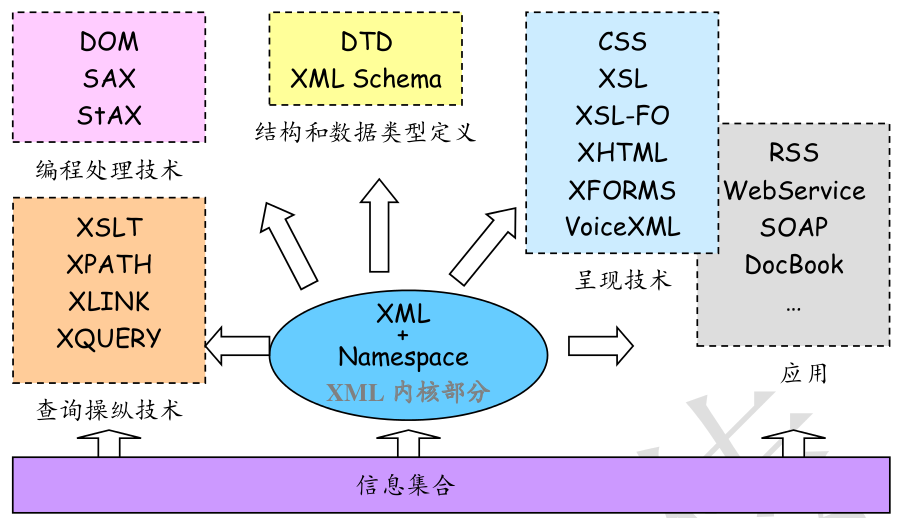
\includegraphics[width=0.9\textwidth]{figure/overview.png}
\end{figure}
\end{frame}

\begin{frame}[fragile]{目录}
\begin{easylist} \easyitem
& XML的起源
& XML的设计目标与特点
& XML技术体系
& XML的应用与发展
& XML相关工具
\end{easylist}
\end{frame}

\subsection{1.1 XML的起源}

\begin{frame}{1.1 XML的起源}
\begin{enumerate}
\item 标记起源
\item 过程标记:RTF
\item 通用编码:TEX
\item SGML
\item XML
\end{enumerate}
\end{frame}

\begin{frame}{标记起源}
\begin{itemize}
\item 标记语言(Markup Language)起源于传统印刷
\item  计算机中的电子标记(WPS、OpenOffice……)
\item 定义: 
\begin{shaded}标记语言就是一种用来给文本添加“格式标注”以指明文档中文本编排格式的语言,一般由定义文档格式的一些规定代码和控制标记组成。\end{shaded}
\end{itemize}
\end{frame}

\begin{frame}{过程标记}
\par 以微软开发的富文本格式 \framebox{RTF: Rich Text Format}为典型代表:
\begin{exampleblock} {例子}
	\par 用Word输入如下文字,并保存为rtf类型:
	\par {\color{red}XML} and RTF!
	\par 用记事本打开保存的文件,查看其文本内容
\end{exampleblock}
\end{frame}

\begin{frame}[fragile]{通用编码}
\par 以\framebox{TeX}为典型代表,例如以下代码片段:
\begin{exampleblock}{TeX示例}
  \begin{lstlisting}[tabsize=8,language=TeX]
  \noindent Tian Xia\par
  \noindent Information Resource Management\par
  \noindent Renmin University of China\par
  \smallskip
  This is a book about XML. It you have some problems, you can concat us directly.\par
  \bye
  \end{lstlisting}
\end{exampleblock}
\end{frame}


\begin{frame}[fragile]{SGML}
\par SGML(Standard Generalized Markup Language), 即标准通用标记语言, 是一种定义电子文档结构和描述其内容的国际标准语言, 早在 Web 发明之前 SGML 就已存在。由IBM的Goldfarb、Mosher 和 Lorie创造。
\par 是HTML、DocBook、XML等新标记语言的基础
\end{frame}


\begin{frame}[fragile, allowframebreaks]{HTML}
\par 1989 年由欧洲量子实验室的研究人员 Tim Berners Lee 在 SGML 的基础上开发的一个简化子集。
\begin{exampleblock}{HTML示例}
  \begin{lstlisting}[tabsize=8,language=HTML]
<html>
    <head>
        <title>HTML网页测试</title>
    </head>
    <body>
        <h1>简单的HTML</h1>
        <p>我的<font color="red">测试网页!</font></p>
    </body>
</html>
  \end{lstlisting}
\end{exampleblock}

\newpage
\par HTML本质上是通过标记的方式,以纯文本形式对网页进行描述,而对标记的解释则由浏览器执行,如现在流行的 IE (Internet Explorer)浏览器、 FireFox 浏览器、 Opera 浏览器等。浏览器读取网页源代码,即 HTML 标记文本,并通过渲染呈现给用户,就形成了用户最终看到的网页。
\begin{exampleblock}{HTML缺点}
\begin{itemize} 
\item 标记固定
\item 标记侧重于如何显示信息,缺乏对数据内容含义的表达能力
\item 缺乏严格的结构要求
\end{itemize}
\end{exampleblock}
\end{frame}


\begin{frame}[fragile, allowframebreaks]{XML}
\par W3C设计,删除了 SGML 中所有不必要的组件, 保留了 SGML 的基本原理: 标记用于描述文档结构; 模型必须与文档相关联。并注重简单性原则。
\par XML示例文档内容:
\begin{lstlisting}[tabsize=8,language=XML]
<?xml version="1.0" encoding="gb2312"?>
<?xml-stylesheet type="text/xsl" href="1-5.xsl"?>
<books>
    <book isbn="7-302-02368-9">
        <title>数据结构</title>
        <author>严蔚敏,吴伟民</author>
        <publisher>清华大学出版社</publisher>
        <price>22.0</price>
    </book>
</books>
\end{lstlisting}

\par XSLT示例文档内容:
\begin{lstlisting}[tabsize=8, basicstyle=\small\tt, language=XML]
<?xml version="1.0" encoding="gb2312"?>
<xsl:stylesheet version="1.0" xmlns:xsl="http://www.w3.org/1999/XSL/Transform">
    <xsl:template match="/">
        <html>
            <head><title>这是图书的呈现样式结果</title></head>
            <body>
                <table border="1">
                <tr>
                    <th>书名 </th>
                    <th>作者 </th>
                    <th>出版社 </th>
                    <th>价格 </th>						
                </tr>					
                <tr>
                    <td><xsl:value-of select="books/book/title"/></td>
                    <td><xsl:value-of select="books/book/author"/></td>
                    <td><xsl:value-of select="books/book/publisher"/></td>
                    <td><xsl:value-of select="books/book/price"/></td>						
                </tr>
                </table>
            </body>
        </html>
    </xsl:template>
</xsl:stylesheet>
\end{lstlisting}

\par {\color{red}用浏览器打开XML文档,查看效果}
\end{frame}


\begin{frame}[fragile]{SGML、HTML 与 XML 的关系}
\begin{figure}
	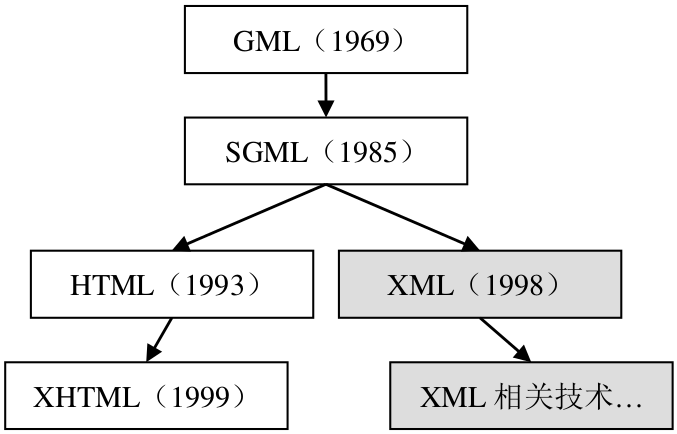
\includegraphics[width=0.8\textwidth]{figure/intro-1.png}
\end{figure}
\end{frame}


\subsection{1.2 XML 的设计目标与特点}


\begin{frame}{XML 的设计目标}
\begin{itemize} 
\item 可以直接应用于因特网
\item 支持各类不同的应用程序
\item 与 SGML 兼容
\item 处理 XML 文件的程序容易编写
\item 选择性功能的数量尽可能少
\item 清晰明了,可读性强
\item 设计应该合乎格式并且简洁
\item 容易创建
\item 标记必须保证其可读性,不能因为过于简化而导致含义模糊
\end{itemize}
\end{frame}


\begin{frame}{XML 的主要特点}
\begin{itemize} 
\item 具有良好的格式
\item 具有验证机制
\item 增强了 Web 应用的灵活性
\item 具有丰富的显示样式
\item 是电子数据交换 EDI 的通用格式
\item 支持复杂的数据关系和快捷的数据处理
\item 具有面向对象的特性
\item 是一种开放的标准
\item 技术体系性强
\end{itemize}

\par 思考XML的不足之处
\end{frame}


\subsection{1.3 XML 技术体系}
\begin{frame}[fragile]{ XML 技术体系}
\begin{figure}
	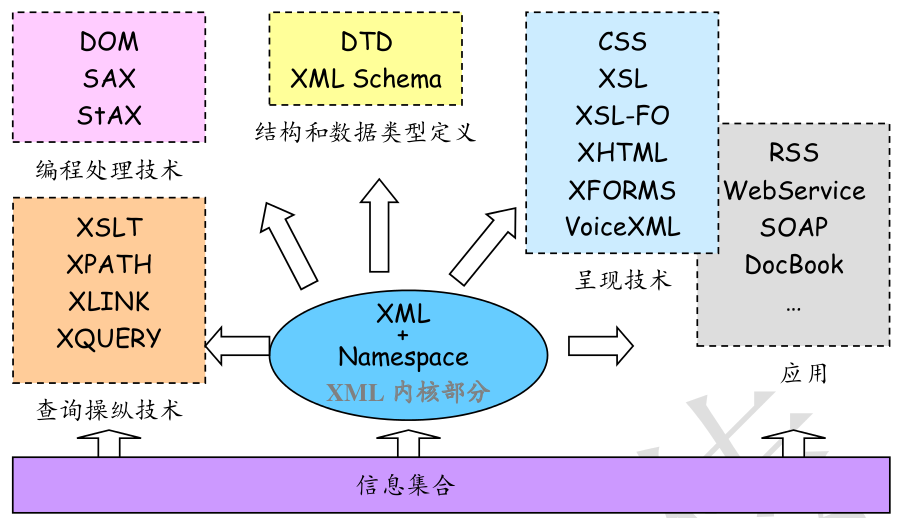
\includegraphics[width=0.8\textwidth]{figure/intro-2.png}
\end{figure}
\end{frame}


\subsection{1.4 XML 的应用与发展}
\begin{frame}[fragile]{ XML 的应用与发展}
\begin{itemize} 
\item 行业标记语言设计领域
\item 电子文件的长期保存领域
\item 电子数据交换领域
\item Web应用领域
\end{itemize}
\end{frame}


\subsection{1.5 XML 相关工具}
\begin{frame}[fragile]{ XML 相关工具}
\begin{itemize} 
\item 编辑工具:文本编辑工具、oXygen XML Editor、XML Spy \dots
\item 浏览工具:浏览器
\item 验证工具:浏览器、专用XML工具和软件包
\item 解析器:Apache Xerces
\end{itemize}
\end{frame}


\begin{frame}[fragile]{ oXygen XML Editor}
\begin{figure}
	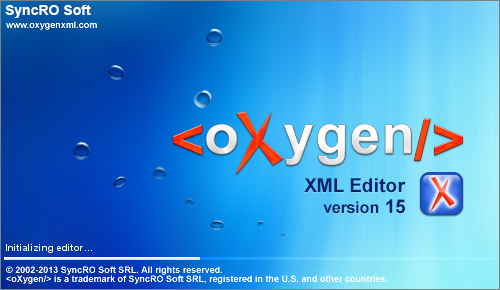
\includegraphics[width=0.8\textwidth]{figure/intro-oxygen.png}
\end{figure}
\begin{shaded}
\par 推荐使用,比XML Spy对标准的支持更好
\end{shaded}
\end{frame}


\begin{frame}[fragile]{ 教材}
\begin{center}
   
\includegraphics[width=0.4\textwidth]{figure/book-cover.png}
\end{center}
\end{frame}


\begin{frame}
\begin{center}
    \Huge END
\end{center}
\begin{figure}
    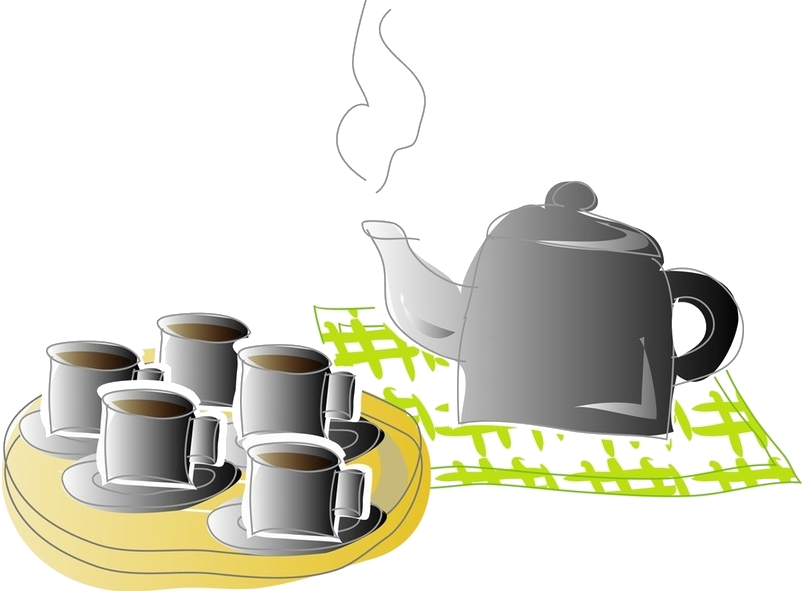
\includegraphics[width=0.75\textwidth]{figure/relax.png}
\end{figure}
\end{frame}

%\section{XML基本语法}

\begin{frame}{CH2 XML基本语法}
\begin{figure}
    
\includegraphics[width=0.9\textwidth]{figure/cover.png}
\end{figure}
\end{frame}

\begin{frame}{本章学习目标}
\begin{itemize}
\item 掌握XML的文档组成结构
\item 掌握XML声明、处理指令、注释、元素、属性、命名空间等基本概念
\item 能够编写格式良好的XML文档
\end{itemize}
\end{frame}

\begin{frame}[fragile]{目录}
\begin{easylist} \easyitem
& XML文档结构
& 元素
&& 元素和标记
&& 元素的内容
&& 元素的嵌套
& 属性
&& 属性的语法形式
&& 属性的使用场景
&& 属性的命名规范
&& 属性值
& 命名空间
& XML文档规范级别
\end{easylist}
\end{frame}

\subsection{2.1 XML文档结构}

\begin{frame}{2.1 XML文档结构}
\par XML本身侧重于数据的表示,并通过CSS、XSLT等技术把数据以指定的格式进行呈现,实现数据表示与呈现的分离。
\end{frame}


\begin{frame}[fragile, allowframebreaks]{示例XML文档}
\begin{lstlisting}[tabsize=8, basicstyle=\small\tt, language=XML]
<?xml version="1.0" encoding="UTF-8" standalone="yes"?>
<?xml-stylesheet type="text/css" href="2-1.css"?>
<!-- 个人通讯录 -->
<addressList>
    <group name="同学">
        <person>
            <name>吴泽林</name>
            <birthday>1985-09-11</birthday>
            <mobile>135-1234-5678</mobile>
            <telephone>68689999</telephone>
            <email>wuzelin@163.com</email>
            <address>漳州</address>
        </person>
    </group>
    <group name="网友">
        <person>
            <name>罗中华</name>
            <mobile>136-1111-1118</mobile>
            <telephone>22339999</telephone>
            <email>luozh@163.com</email>
            <address>北京</address>
        </person>
    </group>
</addressList>

<!-- 处于篇幅考虑,书中源代码内容有删减,读者可以通过附带源码
查看更多信息 -->
\end{lstlisting}
\end{frame}


\begin{frame}{文档构成}
\par 一个XML文档由序言、主体和尾声三部分构成
\begin{itemize}
\item 序言(Prolog): 从XML声明到文档根元素开始前的部分,包括XML声明、注释和处理指令等,序言是可选的
\item 文档主体(Body): 文档根元素及其所包含的内容,每一个XML文档有且仅有一个根元素
\item 尾声(Epilog): 文档根元素后面的部分,可以包含注释、处理指令以及空白信息,一般不出现
\item 一个XML文档最基本的语法要素包括:XML声明、处理指令、注释和XML元素.
\end{itemize}
\end{frame}


\begin{frame}{文档声明}
\begin{shaded}
<?xml version="1.0" encoding="UTF-8" standalone="yes"?>
\end{shaded}

\begin{itemize}
\item version
\item  encoding
\item standalone
\end{itemize}
\end{frame}


\begin{frame}{处理指令}
\begin{shaded}
\par 语法形式: <?处理指令名称 处理指令信息?>
\par E.g. <?topdf path="/pdf-files" ?>
\end{shaded}

\begin{itemize}
\item 处理指令PI(Processing Instruction)是XML文档中为XML处理程序提供必要的处理信息的指令描述。XML解析器会把它原封不动地传递给XML应用程序,由应用程序来根据该指令进行必要处理,或者再把它原封不动地传递给下一个应用程序。
\item  处理指令如何解释完全由外部应用程序决定
\item xml-stylesheet问题
\end{itemize}
\end{frame}


\begin{frame}{注释}
\begin{shaded}
\par 语法形式: <!-- 注释正文 -->
\end{shaded}

\begin{itemize}
\item 注释本身不能放入到标记之内
\item  注释正文中不能出现连续的“--”符号
\item 注释不能以“--->”符号串结尾,也不能放到XML文档声明之前
\item 可以对标记进行注释
\item 注释不能嵌套使用
\end{itemize}
\end{frame}


\begin{frame}[fragile]{注释本身不能放入到标记之内}
\begin{lstlisting}[tabsize=8, basicstyle=\small\tt, language=XML]
<?xml version="1.0" encoding="UTF-8"?>
<document>
    <head <!--This is the heading element-->>
        注释测试例子
    </head>
    <body>正文内容</body>
</document>
\end{lstlisting}
\end{frame}


\begin{frame}[fragile]{注释正文中不能出现连续的“--”符号}
\begin{lstlisting}[tabsize=8, basicstyle=\small\tt, language=XML]
<?xml version="1.0" encoding="UTF-8"?>
<document>
    <head>注释测试例子</head>
    <!--这是正文内容--夏天-->
    <body>正文内容</body>
</document>
\end{lstlisting}
\end{frame}


\begin{frame}[fragile]{注释不能以“--->”结尾,不能放到文档声明之前}
\begin{lstlisting}[tabsize=8, basicstyle=\small\tt, language=XML]
<!-- 该注释后面是XML声明 -->
<?xml version="1.0" encoding="UTF-8"?>
<document>
    <head>注释测试例子</head>
    <!--这是正文内容-夏天--->
    <body>正文内容</body>
</document>
\end{lstlisting}
\end{frame}


\begin{frame}[fragile]{可以对标记进行注释}
\begin{lstlisting}[tabsize=8, basicstyle=\small\tt, language=XML]
<?xml version="1.0" encoding="UTF-8"?>
<document>
    <!--
    <head>注释测试例子</head>
    <body>正文内容</body>
    -->
</document>
\end{lstlisting}
\end{frame}


\begin{frame}[fragile]{注释不能嵌套使用}
\begin{lstlisting}[tabsize=8, basicstyle=\small\tt, language=XML]
<?xml version="1.0" encoding="UTF-8"?>
<document>
    <!--
    <head>注释测试例子</head>
    <!-- 这是正文内容-夏天 -->
    <body>正文内容</body>
    -->
</document>
\end{lstlisting}
\end{frame}



\subsection{2.2 元素}

\begin{frame}{2.2 元素}
\par 元素(Element)是XML文档的基本构成单元,它表示了文档的结构和文档中包含的数据,格式良好的XML文档必须拥有一个唯一的根元素。
\begin{itemize}
\item 元素和标记
\item  元素内容
\item 元素的嵌套
\end{itemize}
\end{frame}

\subsubsection{2.2.1 元素和标记}
\begin{frame}{元素和标记}
\begin{shaded}
\par 元素的基本语法形式: <标记>元素内容</标记>
\par 标记的基本语法形式:<标记名 [[属性名1="属性值1"] [属性名2="属性值2"] …]>
\end{shaded}
\begin{itemize}
    \item 标记区分大小写
    \item  标记必须配对出现
    \item 标记首字符以字母、下划线“\_”、冒号“:”以及Unicode字符集中的某一部分开始,支持汉字; 其他部分可以是字母、数字、下划线“\_”、连字符“-”、句点“.”、冒号“:”,以及Unicode字符集中的某一部分
    \item 标记不能包含空格符号或斜线符号“/”
\end{itemize}
\end{frame}


\begin{frame}{标记示例}
\begin{itemize}
    \item 有效的非空标记示例:<address>漳州</address>
    \item 有效的空标记示例:  <img src="test.jpg"/>
    \item 无效标记示例:      <address>漳州</Address>
    \item 无效标记示例:      <p>段落内容之一<p>段落内容之二
\end{itemize}
\end{frame}


\subsubsection{2.2.2  元素的内容}
\begin{frame}{2.2.2  元素的内容}
\par 元素内容可以包括被解析字符数据(Parsed Character Data)、字符数据CDATA段、以及处理指令和注释
\end{frame}


\begin{frame}{被解析字符数据}
\par 被解析字符数据部分可以是任意合法的Unicode字符,但是不能包含被用作特殊用途的字符,例如标记的开始符号“<”。
\par 通过实体转义的方式解决特殊字符问题
\begin{center}
    \begin{tabular}{|c|c|}
    \Xhline{1.3pt}
    字符 &    引用方式 \\
    \Xhline{1.3pt}
     < & \&lt;  \\
     \hline
     > & \&gt;  \\
    \hline
    \& & \&amp;  \\
    \hline
    ' & \&quot;  \\
    \hline
    " & \&apos;  \\
    \hline
    \end{tabular}
\end{center}
\end{frame}


\begin{frame}[fragile]{给书名加上书名号}
\begin{lstlisting}[tabsize=8, basicstyle=\small\tt, language=XML]
<?xml version="1.0" encoding="UTF-8"?>
<books>
    <book>
        <title>XML原理与应用</title>
        <author>夏天</author>    
    </book>
</books>
\end{lstlisting}
\end{frame}


\begin{frame}{CDATA段}
\begin{shaded} 
\par 基本语法形式: <![CDATA[ 文本内容 ]]>
\par 有利于处理包含大量特殊符号的文本当作普通文本处理的情况
\end{shaded}
\end{frame}

\begin{frame}[fragile]{采用实体转义方式}
\begin{lstlisting}[tabsize=8, basicstyle=\small\tt, language=XML]
<?xml version="1.0" encoding="UTF-8"?>
<demo>
    <content>
        &lt;group name="同学"&gt;
            &lt;person&gt;
                &lt;name&gt;吴泽林&lt;/name&gt;
                &lt;birthday&gt;1985-09-11&lt;/birthday&gt;
                &lt;mobile&gt;135-1234-5678&lt;/mobile&gt;
                &lt;telephone&gt;68689999&lt;/telephone&gt;
                &lt;email&gt;wuzelin@163.com&lt;/email&gt;
                &lt;address&gt;漳州&lt;/address&gt;
            &lt;/person&gt;
        &lt;/group&gt;
    </content>
</demo>
\end{lstlisting}
\end{frame}

\begin{frame}[fragile]{采用CDATA方式}
\begin{lstlisting}[tabsize=8, basicstyle=\small\tt, language=XML]
<?xml version="1.0" encoding="UTF-8"?>
<demo>
    <content>
        <![CDATA[
        <group name="同学">
            <person>
                <name>吴泽林</name>
                <birthday>1985-09-11</birthday>
                <mobile>135-1234-5678</mobile>
                <telephone>68689999</telephone>
                <email>wuzelin@163.com</email>
                <address>漳州</address>
            </person>        
        </group>
        ]]>
    </content>
</demo>
\end{lstlisting}
\end{frame}




\subsubsection{2.2.3 元素的嵌套}
\begin{frame}[fragile]{2.2.3 元素的嵌套}
\begin{easylist} \easyitem
& 元素描述了XML文档的逻辑结构,对于一个复杂的文档来说,单纯用一组并列的元素是无法准确刻画其结构关系的,通过在元素中嵌套子元素可以更好地描述XML文档数据之间的语义关联性。同时,也可以根据元素之间的嵌套关系把整个XML文档看成是一棵具有严格层次关系的树,方便数据的查询、定位和处理。
& XML的元素之间虽然可以嵌套使用,但不能交叉重叠嵌套,例如以下写法是错误的:
& <h1>中国<b>古代文明</h1></b>
\end{easylist}
\end{frame}



\subsection{2.3 属性}

\begin{frame}[fragile]{2.3 属性}
\par 属性是元素的可选组成部分,用于对元素及其内容的附加信息进行说明
\begin{easylist} \easyitem
& 属性的语法形式
& 属性的使用场景
& 属性的命名规则
& 属性值
\end{easylist}
\end{frame}

\subsubsection{2.3.1 属性的语法形式}
\begin{frame}[fragile]{属性的语法形式}
\begin{easylist} \easyitem
& 非空元素如下:
&& <标记名 属性名1="属性值1" 属性名2="属性值2" …] >元素内容</标记名>
&& <标记名 属性名1='属性值1' 属性名2='属性值2' …] />元素内容</标记名>
& 空元素如下:
&& <标记名 属性名1="属性值1" 属性名2="属性值2" … />
&& <标记名 属性名1='属性值1' 属性名2='属性值2' … />
& E.g. <person group="同学"></person>
\end{easylist}

\end{frame}


\subsubsection{2.3.2 属性的使用场景}
\begin{frame}[fragile]{属性的使用场景}
\begin{easylist} \easyitem
& 属性的使用
&& 与XML文档阅读者无关的简单信息建议使用属性
&& 与XML文档有关但是与XML文档的内容无关的简单信息建议使用属性
&& 元素与属性的具体使用有争论,需要灵活掌握
& 属性的不足
&& 属性不能包含多个值(元素可以)
&& 属性不容易被扩充(方便将来的修改)
&& 属性不能描述结构(子元素可以)
&& 属性更难被程序代码处理
&& 属性值不容易进行DTD测试
\end{easylist}
\end{frame}


\subsubsection{2.3.3 属性的命名规则}
\begin{frame}[fragile]{属性的命名规则}
\begin{easylist}
& 属性的命名规则和元素相似
& 同一个元素内不能包含多个同名属性,例如以下反例:\\ <todo date="2050-05-05" date="2150-05-05" />
\end{easylist}
\end{frame}


\subsubsection{2.3.4 属性值}
\begin{frame}[fragile]{属性值}
\begin{easylist}
& 属性值必须用单引号或双引号括起来,不能混用
& 双引号括起来的属性值中可以出现单引号,反之亦然
& 属性值不能直接包括“<”符号,但可以包含''>''
& 属性值不能直接包括“\&”符号,除非引用实体
\end{easylist}
\end{frame}

\begin{frame}[fragile]{非法属性值示例}
\begin{easylist}
& <todo status="important("special")"/>  \\ <!-- 用双引号括起来的字符串中不能直接包含双引号 -->
& <todo status="important > urgent"/>   \\ <!--  属性值中不能直接包含小于号 -->
& <todo status="important \& urgent"/>  \\ <!-- 属性值中不能直接包含“\&” -->
& <todo status="important'/>  \\ <!-- 属性值不能用一个单引号和一个双引号括起来 -->
& <todo status=important/>   \\ <!-- 属性值必须用引号括起来 -->
\end{easylist}
\end{frame}


\subsection{2.4 命名空间}

\begin{frame}[fragile]{命名空间问题}
\par 人力资源维护的员工信息:
\begin{lstlisting}[tabsize=8, basicstyle=\small\tt, language=XML]
<?xml version="1.0"?>
<employees>
    <employee>
        <name>金成</name>
        <birthday>1982-08</birthday>
        <hiredate>2005-09</hiredate>
        <major>软件开发</major>
        <projects>
            <project name="项目A" role="工程师" year="2006"/>
            <project name="项目B" role="架构师" year="2007"/>
        </projects>
    </employee>
</employees>
\end{lstlisting}
\end{frame}


\begin{frame}[fragile]{命名空间问题}
\par 你认为该员工表现优秀,应该增加薪水以示奖励,此时,可在XML文件中增加一条评论:“表现优秀,增加10\%薪水”
\begin{lstlisting}[tabsize=8, basicstyle=\small\tt, language=XML]
<?xml version="1.0"?>
<employees>
    <employee>
        <name>金成</name>
        <birthday>1982-08</birthday>
        <hiredate>2005-09</hiredate>
        <major>软件开发</major>
        <comment>表现优秀,增加10%薪水</comment>
        <projects>
            <project name="项目A" role="工程师" year="2006"/>
            <project name="项目B" role="架构师" year="2007"/>
        </projects>
    </employee>
</employees>
\end{lstlisting}
\end{frame}


\begin{frame}[fragile]{命名空间问题}
\par 人力资源管理人员根据老板的评论,加入了自己的注释
\begin{lstlisting}[tabsize=8, basicstyle=\small\tt, language=XML]
<?xml version="1.0"?>
<employees>
    <employee>
        <name>金成</name>
        <birthday>1982-08</birthday>
        <hiredate>2005-09</hiredate>
        <major>软件开发</major>
        <comment>表现优秀,增加10%薪水</comment>
        <comment>薪水已调整</comment>
        <projects>
            <project name="项目A" role="工程师" year="2006"/>
            <project name="项目B" role="架构师" year="2007"/>
        </projects>
    </employee>
</employees>
\end{lstlisting}
\end{frame}

\begin{frame}[fragile]{问题}
\par 由于老板和人力资源管理人员都可能向原XML文件中增加同样的标记<comment>,日后再来阅读该文件时,便极有可能增加语义混淆:
\begin{easylist}
& 哪一些评论是老板增加的?
& 哪一些是人力部门工作人员增加的?
\end{easylist}
\end{frame}


\begin{frame}[fragile, allowframebreaks]{使用命名空间}
\begin{shaded}
\par 语法形式: xmlns:命名空间前缀="命名空间名"
\end{shaded}
\begin{lstlisting}[tabsize=8, basicstyle=\small\tt, language=XML]
<?xml version="1.0"?>
<hr:employees xmlns:hr="http://www.demo.org/human_resources"
    xmlns:boss="http://www.demo.org/big_boss">
    <hr:employee>
        <hr:name>金成</hr:name>
        <hr:birthday>1982-08</hr:birthday>
        <hr:hiredate>2005-09</hr:hiredate>
        <hr:major>软件开发</hr:major>
        <boss:comment>表现优秀,增加10%薪水</boss:comment>
        <hr:comment>薪水已调整</hr:comment>
        <hr:projects>
            <hr:project name="项目A" role="工程师" year="2006"/>
            <hr:project name="项目B" role="架构师" year="2007"/>
        </hr:projects>
    </hr:employee>
</hr:employees>
\end{lstlisting}
\end{frame}

\begin{frame}{使用命名空间}
\par 根据教材进一步了解默认命名空间和命名空间的作用域
\end{frame}


\subsection{2.5 XML文档的规范级别}

\begin{frame}[fragile]{2.5 XML文档的规范级别}
\begin{easylist} \easyitem
& 格式良好的XML文档
&& 符合XML语法要求
& 有效的XML文档
&& 格式良好,满足约束条件
& 规范化的XML文档
&& 判定两个XML文件在信息集合的角度看是否一致的方法
\end{easylist}
\end{frame}


\begin{frame}
\begin{center}
    \Huge END
\end{center}
\begin{figure}
    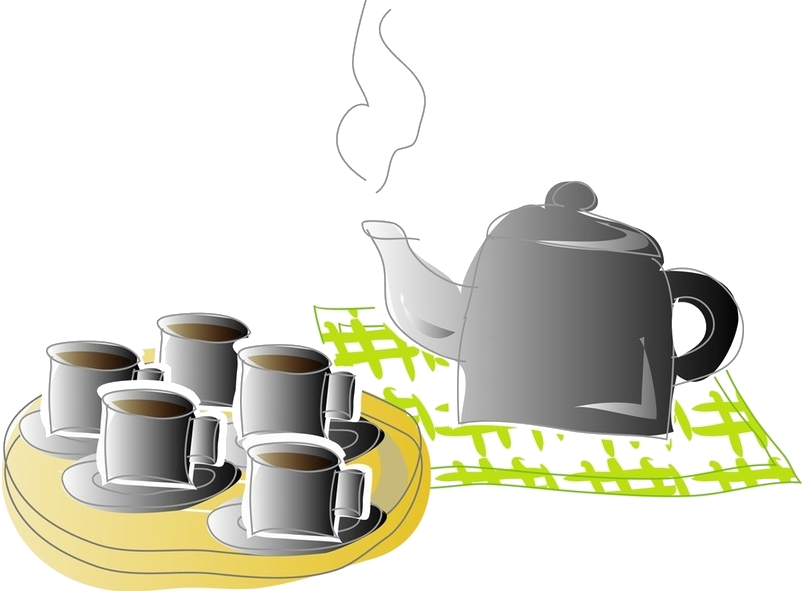
\includegraphics[width=0.75\textwidth]{figure/relax.png}
\end{figure}
\end{frame}

\section{文档类型定义DTD}


\begin{frame}[fragile]{CH3 DTD}
\begin{figure}
    
\includegraphics[width=0.5\textwidth]{figure/dtd.png}
\end{figure}
\end{frame}

\begin{frame}[fragile]{本章学习目标}
\begin{easylist} \easyitem
& 了解 DTD 的作用
& 掌握 DTD 的语法规则和使用方法
& 能够利用 XML 编辑工具实现 DTD 的编辑和验证
\end{easylist}
\end{frame}

\begin{frame}[fragile, allowframebreaks]{目录}
\begin{easylist} \easyitem
& DTD的作用
& DTD的关联方式
&& 内部DTD、外部DTD、公用DTD、内外结合方式
& DTD元素
&& 元素类型声明
&& 空元素
&& 文本类型元素
&& 元素内容模型与混合内容元素
& DTD属性
&& 属性声明
&& 属性类型
&& 属性的默认形态
&& 特殊属性
& DTD实体
&& 实体类型与实体引用
&& 内部可解析通用实体
&& 外部可解析通用实体
&& 外部非解析通用实体
&& 内部参数实体
&& 外部参数实体
& DTD NOTATION
& DTD的包含与忽略
\end{easylist}
\end{frame}

\subsection{3.1 DTD的作用}

\begin{frame}{3.1 DTD的作用}
\par 老师请每一个同学把最近一年看过的5本书写出来,并进行汇总统计,供大家交流学习,要求大家采用XML进行表示,图书信息暂时只包含作者和书名。由于XML表示方式非常自由,不同同学的表示结果很可能不同。
\end{frame}

\begin{frame}[fragile]{第1个同学的XML文档}
\begin{lstlisting}[tabsize=8, basicstyle=\small\tt, language=XML]
<?xml version="1.0"?>
<book>
    <name author="罗贯中">三国演义</name>
    <name author="曹雪芹">红楼梦</name>
    <name author="施耐庵">水浒传</name>
    <name author="吴承恩">西游记</name>
    <name author="荷马">荷马史诗</name>
</book>
\end{lstlisting}
\end{frame}

\begin{frame}[fragile]{第2个同学的XML文档}
\begin{lstlisting}[tabsize=8, basicstyle=\small\tt, language=XML]
<?xml version="1.0"?>
<books>    
    <book title="神曲" author="但丁"/>
    <book title="哈姆雷特" author="莎士比亚"/>
    <book title="浮士德" author="歌德"/>
    <book title="哈克贝利芬历险记" author="马克.吐温"/>
    <book title="少年维特之烦恼" author="歌德"/>
</books>
\end{lstlisting}
\end{frame}

\begin{frame}[fragile]{问题}
\begin{easylist} \easyitem    
& 不同同学所采用的描述方式却不尽相同,这使得后续的自动汇总处理难以实现
& 在实际应用中,“格式良好”仅是一个基本要求,还需要满足一些额外的约束
& DTD通过独特的语法,规定了XML文档编写应遵守的约束
& DTD示例:
\end{easylist}
\begin{lstlisting}[tabsize=8, basicstyle=\small\tt, language=XML]
<!ELEMENT books (book)+>
<!ELEMENT book EMPTY>
<!ATTLIST book 
    title CDATA #REQUIRED
    author CDATA #REQUIRED
>
\end{lstlisting}
\end{frame}



\subsection{3.2 DTD的关联方式}
\begin{frame}[fragile]{3.2 DTD的关联方式}
\begin{easylist} \easyitem    
& 内部DTD
& 外部DTD
& 公用DTD
& 内外结合关联方式
\end{easylist}
\end{frame}

\begin{frame}[fragile]{内部关联方式}
\begin{lstlisting}[tabsize=8, basicstyle=\small\tt, language=XML]
<?xml version="1.0"?>
<!DOCTYPE books [
    <!ELEMENT books (book)+>
    <!ELEMENT book EMPTY>
    <!ATTLIST book 
        title CDATA #REQUIRED
        author CDATA #REQUIRED
    >
]>
<books>    
    <book title="神曲" author="但丁"/>
    <book title="哈姆雷特" author="莎士比亚"/>
    <book title="浮士德" author="歌德"/>
    <book title="哈克贝利芬历险记" author="马克.吐温"/>
    <book title="少年维特之烦恼" author="歌德"/>
</books>
\end{lstlisting}
\end{frame}


\begin{frame}[fragile]{外部关联方式}
\begin{easylist} 
& 当对结构相同的多个XML文档进行验证时,使用外部DTD是最为合适的选择方案
& 既可以使DTD在多个文档中得到复用,方便维护管理,也有利于数据的传输。
\end{easylist}
\end{frame}


\begin{frame}[fragile]{XML文档}
\begin{lstlisting}[tabsize=8, basicstyle=\small\tt, language=XML]
<?xml version="1.0"?>
<!DOCTYPE books SYSTEM "3-2.dtd">
<books>
    <book title="神曲" author="但丁"/>
    <book title="哈姆雷特" author="莎士比亚"/>
    <book title="浮士德" author="歌德"/>
    <book title="哈克贝利芬历险记" author="马克吐温"/>
    <book title="少年维特之烦恼" author="歌德"/>
</books>
\end{lstlisting}
\end{frame}


\begin{frame}[fragile]{DTD文档}
\begin{lstlisting}[tabsize=8, basicstyle=\small\tt, language=XML]
<?xml version="1.0" encoding="UTF-8"?>
<!ELEMENT books (book)+>
<!ELEMENT book EMPTY>
<!ATTLIST book 
    title CDATA #REQUIRED
    author CDATA #REQUIRED
>
\end{lstlisting}
\end{frame}


\begin{frame}[fragile]{公用DTD}
\begin{easylist} 
& 关键字SYSTEM并非关联外部DTD文档的唯一方式, SYSTEM关键字适用于在私有组织内部或个人多个文档之间对DTD的共享使用。使用PUBLIC关键字的公用DTD是另一种常见的关联方式
& XML文档与公用DTD的关联方式
&& <!DOCTYPE 根元素名称 PUBLIC FPI "DTD\_URL">
&& FPI: Formal Public Identifier,规范化公共标识符
\end{easylist}
\end{frame}


\begin{frame}[fragile]{FPI}
\begin{shaded}
\par 初始化字符串//DTD所有者名称//DTD描述//语言标识符
\end{shaded}
\begin{easylist} 
& 初始化字符串
&& 如果DTD是一个ISO标准,则DTD名称以字符串“ISO”开始;
&& 如果DTD由某个非ISO组织所同意,那么名称以“+”开始;
&& 如果没有标准化组织同意该DTD,则名称以“-”开始。
& 例子
\end{easylist}

\begin{lstlisting}[tabsize=8, basicstyle=\small\tt, language=XML]
<!DOCTYPE html PUBLIC "-//W3C//DTD XHTML 1.0 Transitional//EN" 
"http://www.w3.org/TR/xhtml1/DTD/xhtml1-transitional.dtd">

<!DOCTYPE CONTACTS PUBLIC "-//xiatian//Contact Data//EN"
                "http://www.mydomain.com/dtds/contacts.dtd">
\end{lstlisting}
\end{frame}


\begin{frame}[fragile]{内外结合方式}
\begin{easylist} 
& 内部DTD和外部DTD合并使用
\end{easylist}
\end{frame}

\begin{frame}[fragile]{E.g. 外部DTD}
\begin{lstlisting}[tabsize=8, basicstyle=\small\tt, language=XML]
<?xml version="1.0" encoding="UTF-8"?>
<!ELEMENT universities (university)+>
<!ELEMENT university (#PCDATA)>
<!ENTITY RUC "中国人民大学">
\end{lstlisting}
\end{frame}

\begin{frame}[fragile]{E.g. XML文档}
\begin{lstlisting}[tabsize=8, basicstyle=\small\tt, language=XML]
<?xml version="1.0"?>
<!DOCTYPE universities SYSTEM "3-5.dtd"[
    <!ENTITY RUC "人民大学">
]>
<universities>    
    <university>&RUC;</university>
    <university>北京大学</university>
    <university>清华大学</university>
</universities>
\end{lstlisting}

\begin{easylist} 
& 同时使用了外部DTD和内部DTD定义方式
& 内部DTD会覆盖外部DTD已有定义
\end{easylist}
\end{frame}



\subsection{3.3 DTD元素}
\begin{frame}[fragile]{3.3 DTD元素}
\begin{easylist} \easyitem    
& 元素类型声明
& 空元素
& 文本类型元素
& 元素内容模型与混合内容元素
\end{easylist}
\end{frame}


\subsubsection{3.3.1 元素类型声明}
\begin{frame}[fragile]{3.3.1 元素类型声明}
\begin{shaded}
\par 语法:<!ELEMENT 元素名称 元素内容规范>
\end{shaded}

\begin{easylist} \easyitem    
& ELEMENT作为关键字,用于对指定元素进行声明
& ELEMENT单词必须全部大写
& ELEMENT与“<!”之间不能留有空格
& 元素内容规范指明了元素内可以包含的内容形式
&& 空元素(EMPTY)
&& 任意元素(ANY)
&& 父元素
&& 文本元素
&& 混合元素
\end{easylist}
\end{frame}


\begin{frame}[fragile]{Example}
\begin{lstlisting}[tabsize=8, basicstyle=\small\tt, language=XML]
<?xml version="1.0" encoding="UTF-8"?>
<!ELEMENT books ANY>
<!ELEMENT book (title, author, publish)>
<!ELEMENT title (#PCDATA)>
<!ELEMENT author (#PCDATA)>
<!ELEMENT publish (#PCDATA|ISBN)*>
<!ELEMENT ISBN EMPTY>
\end{lstlisting}
\end{frame}


\subsubsection{3.3.2 空元素}
\begin{frame}[fragile]{3.3.2 空元素}
\begin{easylist} \easyitem
& 语法
\begin{lstlisting}[tabsize=8, basicstyle=\small\tt, language=XML, numbers=none]
<!ELEMENT 元素名 EMPTY>
\end{lstlisting}
& 例子
\begin{lstlisting}[tabsize=8, basicstyle=\small\tt, language=XML]
<!ELEMENT 人物 EMPTY>
<!ELEMENT IMG EMPTY>
\end{lstlisting}

& 使用场景
&& 元素把全部数据放在属性里,而元素本身没有任何PCDATA内容
&& 例如:
\begin{lstlisting}[tabsize=8, basicstyle=\small\tt, language=XML]
<人物 姓名="林冲" 籍贯="东京" 职业="强盗" 特长="枪棒"/>
<img src="baby.jpg" alt="baby" title="宝贝的照片"/>
\end{lstlisting}
\end{easylist}
\end{frame}


\subsubsection{3.3.3 文本类型元素}
\begin{frame}[fragile]{3.3.3 文本类型元素}
\begin{easylist} \easyitem    
& 语法:
\begin{lstlisting}[tabsize=8, basicstyle=\small\tt, language=XML]
<!ELEMENT 元素名 (#PCDATA) >
\end{lstlisting}

& 例子
\begin{lstlisting}[tabsize=8, basicstyle=\small\tt, language=XML]
<!ELEMENT 姓名 (#PCDATA)>
<!ELEMENT 籍贯 (#PCDATA)>
\end{lstlisting}

&& \#PCDATA为元素数据的指定类型
&&& Parsed Character Data:可解析字符数据
&&& 元素把全部数据放在属性里,本身没有任何PCDATA内容

& DTD类型限制
&& 不能区分文本和数字,无法区分整数和实数
&& 不能定义用户数据类型
&& 不能限制数据的取值范围
\end{easylist}
\end{frame}


\begin{frame}[fragile]{以下定义方式是否正确?}
\begin{lstlisting}[tabsize=8, basicstyle=\small\tt, language=XML]
<!ELEMENT 姓名 #PCDATA>
<!ELEMENT 姓名 PCDATA>
\end{lstlisting}

\end{frame}


\subsubsection{3.3.4 元素内容模型与混合内容元素}
\begin{frame}[fragile]{3.3.4 元素内容模型与混合内容元素}
\begin{shaded}
\par 元素内容模型ECM(Element Content Models)就是用来描述元素内具体可以包含哪些子元素的一组正则表达式
\end{shaded}
\begin{table}[!hbp] 
\begin{tabular}{|c|c|c|}
\Xhline{1.3pt}
元字符 & 用法 & 范例 \\
\Xhline{1.3pt}
, & 将各个元素依指定顺序排列 & (A,B,C) \\
\hline
字符串 &  一个元素仅能出现一次 &  (A) \\
\hline
* & 元素可以出现0次或0次以上 & A*\\
\hline
+ & 元素可以出现1次或1次以上 & A+\\
\hline
? & 一个元素可以出现0次或一次 & A? \\
\hline
( ) & 分组符号,常结合“,”或“|”使用 &  (A,B) \\
\hline
|  &  逻辑或,只能出现符号作用范围的任一元素1次 & (A|B|C)\\
\hline
\end{tabular}
\caption{元素内容模型的元字符以及相应用法与范例}
\end{table}
\end{frame}


\begin{frame}[fragile]{具有严格顺序的子元素序列}
\begin{shaded}
对内容规范为逗号分隔的子元素序列,文档必须严格按照规定的顺序来书写子元素
\end{shaded}

\begin{lstlisting}[tabsize=8, basicstyle=\small\tt, language=XML]
<?xml version="1.0" encoding="UTF-8" standalone="yes"?>
<!DOCTYPE person [
    <!ELEMENT person (name, telephone, email)>
    <!ELEMENT name (#PCDATA)>
    <!ELEMENT email (#PCDATA)>
    <!ELEMENT telephone (#PCDATA)>    
]>
<person>
    <name>Summer</name>
    <email>summer@ruc.edu.cn</email>
    <telephone>010-82500673</telephone>    
</person>
\end{lstlisting}
\begin{easylist} \easyitem    
& 思考以上XML是否有效?
\end{easylist}
\end{frame}


\begin{frame}[fragile]{可重复元素}
\begin{easylist} \easyitem    
& 若某子元素名后跟有星号“*”或加号“+”,则该元素可以重复若干次
& +代表出现1到多次,即至少出现一次
& *代表出现0到多次,即可以不出现
\end{easylist}

\begin{lstlisting}[tabsize=8, basicstyle=\small\tt, language=XML]
<?xml version="1.0" encoding="UTF-8" standalone="yes"?>
<!DOCTYPE person [
    <!ELEMENT person (name, telephone, email+)>
    <!ELEMENT name (#PCDATA)>
    <!ELEMENT email (#PCDATA)>
    <!ELEMENT telephone (#PCDATA)>    
]>
<person>
    <name>Summer</name>
    <telephone>010-82500673</telephone>    
    <email>summer@ruc.edu.cn</email>
    <email>xia@ruc.edu.cn</email>
</person>
\end{lstlisting}
\end{frame}


\begin{frame}[fragile]{分组与逻辑或}
\begin{easylist} \easyitem    
& 逻辑或“|”用于多选一情况,经常与分组符号“( )”结合使用
& Eaxmple:
\begin{lstlisting}[tabsize=8, basicstyle=\small\tt, language=XML, numbers=none]
<!ELEMENT person (name, (telephone | email) )>
\end{lstlisting}

&& 元素person的子元素name后面只能有一个telephone元素或者email元素,而不能两个都有。
&& 错误写法: 
\begin{lstlisting}[tabsize=8, basicstyle=\small\tt, language=XML, numbers=none]
<!ELEMENT person (name, telephone | email )>
\end{lstlisting}

& 以下DTD语句的含义是什么?
\begin{lstlisting}[tabsize=8, basicstyle=\small\tt, language=XML, numbers=none]
 <!ELEMENT person (name, (telephone | email | (telephone, email) ) )>
\end{lstlisting}

\end{easylist}
\end{frame}


\begin{frame}[fragile]{可选元素}
\begin{easylist} \easyitem    
& 子元素后面跟有问号符号“?”,属于可选元素,可以出现0次或1次
& 当无法确定一个元素是否会出现而且就算出现也只出现一次,可以使用该符号
& E.g. 
\begin{lstlisting}[tabsize=8, basicstyle=\small\tt, language=XML, numbers=none]
<!ELEMENT person (name, (areaCode?, telephone), email )>
\end{lstlisting}
&& person元素中的联系电话部分必须出现telephone子元素,而区号areaCode,则可以出现,也可以不出现
\end{easylist}
\end{frame}


\begin{frame}[fragile]{混合内容}
\begin{easylist} \easyitem    
& 假设采用XML对人物信息进行描述,描述内容采用文本形式,但同时希望文本内出现的人物姓名、籍贯、职业等信息采用元素方式进行结构化表示,也就是说,子元素可以任意散布在一段段的文本之中。
& 可采用混合内容描述方法:
\begin{lstlisting}[tabsize=8, basicstyle=\small\tt, language=XML, numbers=none]
<!ELEMENT 元素名 (#PCDATA | 子元素1 | 子元素2 | … | 子元素n)* >
\end{lstlisting}
\end{easylist}
\end{frame}


\begin{frame}[fragile]{混合内容示例}
\begin{lstlisting}[tabsize=8, basicstyle=\small\tt, language=XML]
<?xml version="1.0" encoding="UTF-8" standalone="yes"?>
<!DOCTYPE 人物 [
    <!ELEMENT 人物 (#PCDATA|姓名|籍贯|职业|特长)* >
    <!ELEMENT 姓名 (#PCDATA)>
    <!ELEMENT 籍贯 (#PCDATA)>
    <!ELEMENT 职业 (#PCDATA)>
    <!ELEMENT 特长 (#PCDATA)>
]>
<人物>
    <姓名>林冲</姓名>,<籍贯>东京</籍贯>人氏,人称豹子头,
官方认定其为水泊梁山<职业>强盗</职业>。
生性耿直,爱交好汉,擅长<特长>枪棒</特长>。
</人物>
\end{lstlisting}

\begin{easylist} \easyitem    
& <!ELEMENT 人物 (\#PCDATA|姓名|籍贯|职业|特长)* >
\end{easylist}
\end{frame}



\subsection{3.4 DTD属性}
\begin{frame}[fragile]{3.4 DTD属性}
\begin{easylist} \easyitem    
& 属性声明
& 属性类型
& 属性的默认形态
& 特殊属性
\end{easylist}
\end{frame}


\subsubsection{3.4.1 属性声明}
\begin{frame}[fragile]{3.4.1 属性声明}
\begin{easylist} \easyitem    
& 语法:
\begin{lstlisting}[tabsize=8, basicstyle=\small\tt, language=XML, numbers=none]
<!ATTLIST 元素名  属性名  属性类型  缺省声明  (属性名 属性类型 缺省声明… ) >
\end{lstlisting}

&& 元素名指明了属性所属的元素名称
&& 属性名表示指定属性的名称
&& 属性类型决定了属性值应具备的类型,如常用的CDATA
&& 缺省声明规定对属性值的要求和指定默认值
\end{easylist}
\end{frame}


\begin{frame}[fragile]{属性声明示例}
\begin{easylist} \easyitem    
& 如下XML文档片段如何声明对应的DTD?
\begin{lstlisting}[tabsize=8, basicstyle=\small\tt, language=XML, numbers=none]
<人物 姓名="林冲"/>
\end{lstlisting}
\end{easylist}
\end{frame}

\begin{frame}[fragile]{属性声明示例}
\begin{easylist} \easyitem    
& 声明方式:
\begin{lstlisting}[tabsize=8, basicstyle=\small\tt, language=XML]
<!ELEMENT 人物 EMPTY>
<!ATTLIST 人物 姓名 CDATA  #REQUIRED >
\end{lstlisting}

&& <!ELEMENT>标记声明“人物”元素为一个空元素
&& <!ATTLIST>标记表明了“人物”元素拥有属性“姓名”,
&& 人物属性类型为CDATA
&& 人物属性使用时必须指明。
\end{easylist}
\end{frame}



\begin{frame}[fragile]{属性简写方式}
\begin{easylist} \easyitem    
& XML:
\begin{lstlisting}[tabsize=8, basicstyle=\small\tt, language=XML, numbers=none]
<人物 姓名="林冲" 籍贯="东京" 职业="强盗" 特长="枪棒"/>
\end{lstlisting}

& 属性逐个声明方式:
\begin{lstlisting}[tabsize=8, basicstyle=\small\tt, language=XML]
<!ELEMENT 人物 EMPTY>
<!ATTLIST 人物    姓名 CDATA #REQUIRED >
<!ATTLIST 人物    籍贯 CDATA #IMPLIED >
<!ATTLIST 人物    职业 CDATA #IMPLIED >
<!ATTLIST 人物    特长 CDATA "武术" >
\end{lstlisting}

& 属性一起声明方式:
\begin{lstlisting}[tabsize=8, basicstyle=\small\tt, language=XML]
<!ATTLIST 人物    姓名 CDATA #REQUIRED
                籍贯 CDATA #IMPLIED
                职业 CDATA #IMPLIED
                特长 CDATA "武术">
\end{lstlisting}
\end{easylist}
\end{frame}


\subsubsection{3.4.2 属性类型}
\begin{frame}[fragile]{3.4.2 属性类型}
\begin{table}[!htp] 
\begin{tabular}{|c|l|}
\Xhline{1.3pt}
类型 & 含义 \\
\Xhline{1.3pt}
CDATA & 属性值为任意合法的字符串,最为常用的属性类型 \\ \hline
Enumerated & 从若干个指定值列表中选择正确的值 \\ \hline
ID &  属性值必须唯一,不能与中其他ID类型属性取相同值 \\ \hline
IDREF & 属性值引用了某一个已经指定的ID类型的属性值 \\ \hline
IDREFS & 属性值由多个IDREF类型的属性值组成,并由空格隔开  \\ \hline
NMTOKEN & Name Token,由符合标记命名要求的字符串组成\\ \hline
NMTOKENS & 该属性值是由空格分隔的一系列NMTOKEN的集合 \\ \hline
ENTITY & 属性值为已经由DTD声明的实体名称  \\ \hline
ENTITIES & 属性值是由空格分隔的一系列ENTITY的集合 \\ \hline
NOTATION & 属性值必须匹配NOTATION名称列表中的某个名称 \\     \hline
\end{tabular}
\caption{DTD的属性类型}
\end{table}
\end{frame}


\begin{frame}[fragile]{CDATA属性类型}
\begin{easylist} \easyitem    
& 字符数据(Character DATA),是最基本的属性类型
& 属性值为不包含小于号“<”和“&”的任意文本字符串
& 如出现“<”和“\&”,需要转义
\begin{lstlisting}[tabsize=8, basicstyle=\small\tt, language=XML]
<?xml version="1.0" encoding="UTF-8" standalone="yes"?>
<!DOCTYPE todolist [
    <!ELEMENT todolist (todo)*>
    <!ELEMENT todo EMPTY>
    <!ATTLIST todo content CDATA #REQUIRED> 
]>
<todolist>
    <todo content="当股价>100的时候抛出'全聚德'"/>
    <todo content="周六&amp;周日回山东临朐"/>
</todolist>
\end{lstlisting}
\end{easylist}
\end{frame}


\begin{frame}[fragile]{Enumerated枚举类型}
\begin{easylist} \easyitem    
& 语法:
\begin{lstlisting}[tabsize=8, basicstyle=\small\tt, language=XML, numbers=none]
<!ATTLIST 元素名 属性名 (属性值1 | 属性值2 | … | 属性值n) 缺省声明>
\end{lstlisting}
& 例子:
\begin{lstlisting}[tabsize=8, basicstyle=\small\tt, language=XML, numbers=none]
<!ATTLIST 交易    货币单位 (人民币 | 日元 | 美元 | 欧元 | 英镑)  "人民币">
\end{lstlisting}
\end{easylist}
\end{frame}


\begin{frame}[fragile]{NOTATION符号类型}
\begin{lstlisting}[tabsize=8, basicstyle=\small\tt, language=XML]
<!ELEMENT 图片 (#PCDATA)>
<!NOTATION gif SYSTEM "IMAGE/gif">
<!NOTATION jpg SYSTEM "IMAGE/jpeg">
<!NOTATION png SYSTEM "IMAGE/png">
<!ATTLIST 图片 格式 NOTATION (gif | jpg | png) #REQUIRED>

<图片 格式="png"/>
\end{lstlisting}
\end{frame}


\begin{frame}[fragile]{ID、IDREF与IDREFS属性类型}
\begin{easylist} \easyitem    
& ID: 
&& 该类型的属性无缺省值,缺省声明必须为\#REQUIRED或\#IMPLIED
&& 一个元素不能拥有超过一个ID类型的属性
& IDREF(ID Reference)
&& 对ID的引用,当某个属性引用了另一个ID类型的属性值时,可将其声明为IDREF
& IDREFS(ID References)
&& 多个标识符的引用,属性值引用了多个由空格分隔的ID类型的属性值
\end{easylist}
\end{frame}


\begin{frame}[fragile]{ID、IDREF与IDREFS示例}
\begin{lstlisting}[tabsize=8, basicstyle=\small\tt, language=XML]
<?xml version="1.0" encoding="UTF-8" standalone="yes"?>
<!DOCTYPE 班级 [
    <!ELEMENT 班级 (学生)*>
    <!ELEMENT 学生 (#PCDATA)>    
    <!ATTLIST 班级 名称 CDATA #REQUIRED>
    <!ATTLIST 班级 班长 IDREF #IMPLIED>
    <!ATTLIST 班级 班委 IDREFS #IMPLIED>
    <!ATTLIST 学生 学号 ID #REQUIRED>
]>
<班级 名称="政务信息一班" 班长="S001" 班委="S001 S002 S004">
    <学生 学号="S001">姜海明</学生>
    <学生 学号="S002">李学健</学生>
    <学生 学号="S003">方路</学生>
    <学生 学号="S004">刘杨</学生>
</班级>
\end{lstlisting}
\end{frame}


\begin{frame}[fragile]{NMTOKEN与NMTOKENS属性类型}
\begin{easylist} \easyitem    
& NMTOKEN: Name Token
&& 限定属性值为有效的XML名称
& NMTOKENS: Name Tokens
&& 一组NMTOKEN类型的字符串,每个NMTOKEN之间以空格分隔
\begin{lstlisting}[tabsize=8, basicstyle=\small\tt, language=XML]
<!ELEMENT 数据 (#PCDATA) >
<!ATTLIST 数据    授权用户 NMTOKENS #IMPLIED>

<数据 授权用户="Lucy Summer Macy">如何学好XML的超级技巧……</数据>
\end{lstlisting}
\end{easylist}
\end{frame}


\begin{frame}[fragile]{ENTITY与ENTITIES属性类型}
\begin{easylist} \easyitem    
& ENTITY
&& 限定属性值为已经声明过的实体名称,
& ENTITIES
&& 可以包含多个实体,实体之间通过空格进行分隔。
\end{easylist}
\end{frame}


\begin{frame}[fragile]{ENTITY与ENTITIES示例}
\begin{lstlisting}[tabsize=8, basicstyle=\small\tt, language=XML]
<?xml version="1.0" encoding="UTF-8"?>
<!DOCTYPE 高校列表 [
    <!ELEMENT 高校列表 (高校)*>
    <!ELEMENT 高校 (#PCDATA)>
    <!ATTLIST 高校 LOGO ENTITY #REQUIRED
                   校园风景 ENTITIES #IMPLIED>
    <!NOTATION JPG SYSTEM "image/jpeg">
    <!ENTITY LOGO2 SYSTEM "ruc_logo.jpg" NDATA JPG>
    <!ENTITY 风景_人大_1 SYSTEM "ruc_1.jpg" NDATA JPG>
    <!ENTITY 风景_人大_2 SYSTEM "ruc_2.jpg" NDATA JPG>
]>
<高校列表>
    <高校 LOGO="LOGO2" 校园风景="风景_人大_1 风景_人大_2">人民大学</高校>
</高校列表>
\end{lstlisting}
\end{frame}


\subsubsection{3.4.3 属性的默认形态}
\begin{frame}[fragile]{3.4.3 属性的默认形态}
\begin{easylist} \easyitem    
& \#REQUIRED
&& 与该属性关联的元素必须为属性指定一个明确的值,不能缺省
& \#IMPLIED
&& 可有可无的属性
& \#FIXED
&& 固定值,不能更改
& 默认值
&& 属性具有一个指定的默认值,与\#FIXED不同,用户可以通过设置元素的属性值,改变其默认值。
\end{easylist}
\end{frame}


\begin{frame}[fragile]{FIXED与默认值}
\begin{lstlisting}[tabsize=8, basicstyle=\small\tt, language=XML]
<!ATTLIST person gender CDATA #FIXED "男">

<person gender="男"/>      <!-- 正确 -->
<person/>                 <!-- 正确,person拥有属性gender,其值为男-->
<person gender="女"/>      <!-- 非法使用-->
\end{lstlisting}

\begin{lstlisting}[tabsize=8, basicstyle=\small\tt, language=XML]
<!ATTLIST person gender CDATA "男">

<person gender="男"/>      <!-- 正确 -->
<person/>                 <!-- 正确,person拥有属性gender,其值为男-->
<person gender="女"/>      <!-- 正确,属性gender值为女-->
\end{lstlisting}
\end{frame}


\subsubsection{3.4.4 XML特殊属性}
\begin{frame}[fragile]{3.4.4 XML特殊属性}
\begin{easylist} \easyitem    
& XML为所有元素预留了三个特殊属性
&& xml:lang — 语种选择
&& xml:space — 白空符处理
&& xml:id — 标识符
\end{easylist}
\end{frame}



\subsection{3.5 DTD实体}
\begin{frame}[fragile]{3.5 DTD实体}
\begin{shaded}实体有利于快速更替特定文字,简化编写和方便修改\end{shaded}

\begin{easylist} \easyitem    
& 实体类型与实体引用
& 内部可解析通用实体
& 外部可解析通用实体
& 外部非解析通用实体
& 内部参数实体
& 外部参数实体
\end{easylist}
\end{frame}


\subsubsection{3.5.1 实体类型与实体引用}
\begin{frame}[fragile]{3.5.1 实体类型与实体引用}
\begin{easylist} \easyitem    
& 1. 通用实体和参数实体
&& 通用实体:  实体只能在XML文档中被引用,不能在DTD中引用
&& 参数实体: 实体只能在DTD中被引用,不能在XML文档中引用
& 2. 内部实体和外部实体
&& 内部实体: 实体值以内嵌方式定义
&& 外部实体: 实体值包含在外部资源中
& 3. 可解析实体和非解析实体
&& 可解析实体: 实体值被XML处理程序解析为XML/DTD文档
&& 非解析实体: 实体值不能被XML处理程序解析
\end{easylist}
\end{frame}


\begin{frame}[fragile]{五种DTD实体类型}
\begin{easylist} \easyitem    
& 内部可解析通用实体
\begin{lstlisting}[tabsize=8, basicstyle=\small\tt, language=XML, numbers=none]
<!ENTITY name "value" >
\end{lstlisting}

& 外部可解析通用实体
\begin{lstlisting}[tabsize=8, basicstyle=\small\tt, language=XML, numbers=none]
<!ENTITY name SYSTEM URI > ……
\end{lstlisting}

& 外部非解析通用实体
\begin{lstlisting}[tabsize=8, basicstyle=\small\tt, language=XML, numbers=none]
<!ENTITY name SYSTEM URI NDATA type> ……
\end{lstlisting}

& 内部参数实体
\begin{lstlisting}[tabsize=8, basicstyle=\small\tt, language=XML, numbers=none]
<!ENTITY \% name "value" >
\end{lstlisting}

& 外部参数实体
\begin{lstlisting}[tabsize=8, basicstyle=\small\tt, language=XML, numbers=none]
<!ENTITY \% name SYSTEM URI > ……
\end{lstlisting}
\end{easylist}
\end{frame}


\begin{frame}[fragile]{实体引用方法}
\begin{easylist} \easyitem    
& 可解析通用实体
\begin{lstlisting}[tabsize=8, basicstyle=\small\tt, language=XML, numbers=none]
&实体名称;
\end{lstlisting}

& 非解析通用实体
\begin{lstlisting}[tabsize=8, basicstyle=\small\tt, language=XML, numbers=none]
属性名称="实体名称" (属性限定为ENTITY或ENTITIES类型)
\end{lstlisting}

& 参数实体
\begin{lstlisting}[tabsize=8, basicstyle=\small\tt, language=XML, numbers=none]
%实体名称; 
\end{lstlisting}
\end{easylist}
\end{frame}

\begin{frame}[fragile]{实体语法示意图}
\begin{figure}
    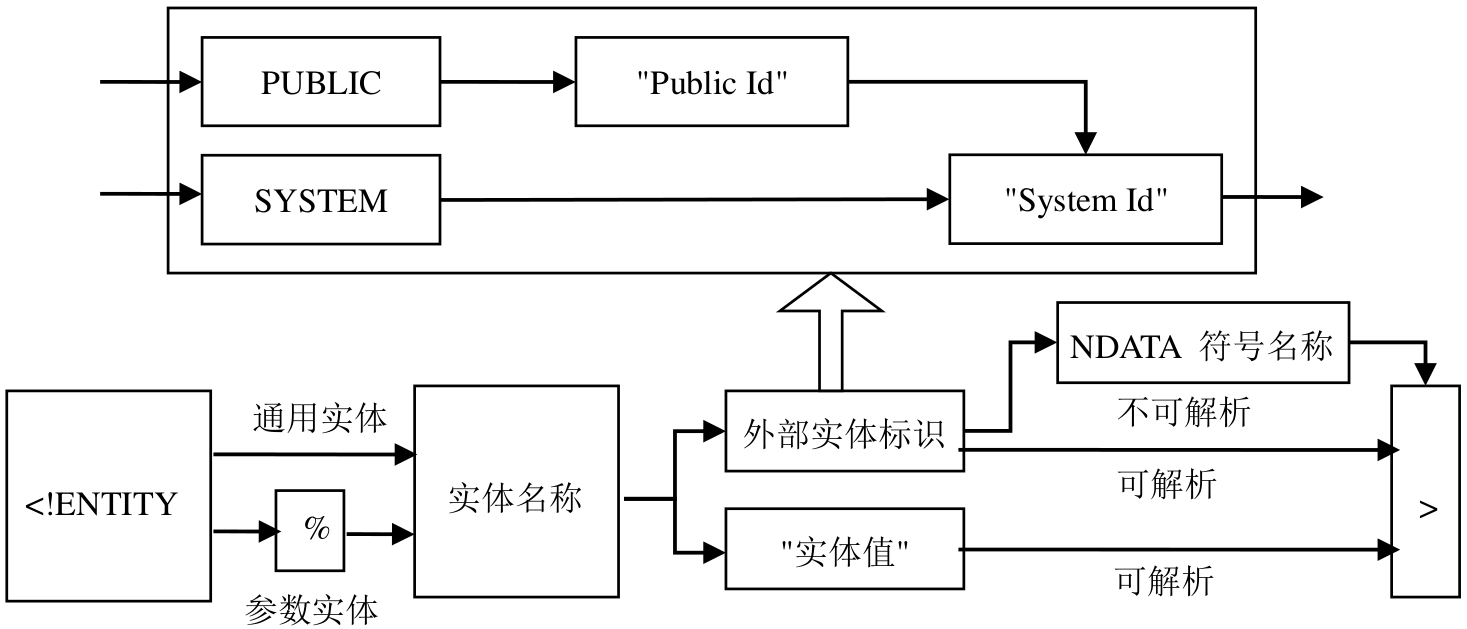
\includegraphics[width=0.9\textwidth]{figure/dtd-entity.png}
\end{figure}
\end{frame}



\subsubsection{3.5.2 内部可解析通用实体}
\begin{frame}[fragile]{3.5.2 内部可解析通用实体}
\begin{easylist} \easyitem    
& 语法形式:
\begin{lstlisting}[tabsize=8, basicstyle=\small\tt, language=XML, numbers=none]
<!ENTITY 实体名称 "实体值" >
\end{lstlisting}

& 例子
\begin{lstlisting}[tabsize=8, basicstyle=\small\tt, language=XML, numbers=none]
<?xml version = "1.0" encoding="utf-8"?>
<!DOCTYPE 数据 [
    <!ELEMENT 数据 (#PCDATA)>
    <!ENTITY 版权声明 "自由信息,由人民大学编写"> 
]>
<数据>&版权声明;</数据>
\end{lstlisting}
\end{easylist}
\end{frame}


\begin{frame}[fragile]{示例}
\begin{easylist} \easyitem    
& 可在实体的定义之中引用已定义实体
\begin{lstlisting}[tabsize=8, basicstyle=\small\tt, language=XML]
<!ENTITY 机构 "人民大学">
<!ENTITY 版权声明 "自由信息,由&机构;编写">
\end{lstlisting}

& 不可以相互引用,如:
\begin{lstlisting}[tabsize=8, basicstyle=\small\tt, language=XML]
<!ENTITY 机构 "人民大学, &版权声明;">
<!ENTITY 版权声明 "自由信息,由&机构;编写">
\end{lstlisting}

& 不能针对DTD的元素定义采用通用实体引用
\begin{lstlisting}[tabsize=8, basicstyle=\small\tt, language=XML]
<!ENTITY 教师基本信息 "(姓名, 性别, 出生年月, 研究方向)">
<!ELEMENT 教授 &教师基本信息;>
<!ELEMENT 副教授 &教师基本信息;>
<!ENTITY 讲师 &教师基本信息;>
\end{lstlisting}
\end{easylist}
\end{frame}


\subsubsection{3.5.3 外部可解析通用实体}
\begin{frame}[fragile]{3.5.3 外部可解析通用实体}
\begin{easylist} \easyitem    
& 语法形式:
\begin{lstlisting}[tabsize=8, basicstyle=\small\tt, language=XML, numbers=none]
<!ENTITY 实体名称 SYSTEM "系统标识符" >  
\end{lstlisting}
\begin{lstlisting}[tabsize=8, basicstyle=\small\tt, language=XML, numbers=none]
<!ENTITY 实体名称 PUBLIC FPI "公共标识符" >
\end{lstlisting}

& 例子
\begin{lstlisting}[tabsize=8, basicstyle=\small\tt, language=XML]
<?xml version = "1.0" encoding="utf-8"?>
<!DOCTYPE 数据 [
    <!ELEMENT 数据 (#PCDATA)>
    <!ENTITY 介绍数据 SYSTEM "intro.txt">    
]>
<数据>&介绍数据;</数据>
\end{lstlisting}
\end{easylist}
\end{frame}


\subsubsection{3.5.4 外部非解析通用实体}
\begin{frame}[fragile]{3.5.4 外部非解析通用实体}
\begin{easylist} \easyitem    
& 外部可解析通用实体可以把外部文件中的文本内容与DTD实体建立关联,并被XML解析器读取处理;
& 对于图片、音频、视频等二进制文件,如果在实体引用时仍然被解析,则会因特殊字符的存在而导致语法错误,为此,W3C引入了非解析实体(Unparsed Entity)概念
& 外部非解析通用实体的语法形式:
\begin{lstlisting}[tabsize=8, basicstyle=\small\tt, language=XML, numbers=none]
<!ENTITY 实体名称 SYSTEM "系统标识符" NDATA Type>
\end{lstlisting}
\begin{lstlisting}[tabsize=8, basicstyle=\small\tt, language=XML, numbers=none]
<!ENTITY 实体名称 PUBLIC FPI "公共标识符" NDATA Type>
\end{lstlisting}
&& Type代表实体类型,为已声明的NOTATION
\end{easylist}
\end{frame}


\begin{frame}[fragile]{外部非解析通用实体示例}
\begin{lstlisting}[tabsize=8, basicstyle=\small\tt, language=XML]
<?xml version = "1.0" encoding="utf-8"?>
<!DOCTYPE 数据 [
    <!ELEMENT 数据 (#PCDATA)>
    <!NOTATION JPG SYSTEM "image/jpeg">
    <!ENTITY 插图 SYSTEM "ruc_1.jpg" NDATA JPG>    
    <!ATTLIST 数据 插图 ENTITY #IMPLIED>    
]>
<数据 插图="插图">外部非解析通用实体示例</数据>
\end{lstlisting}
\end{frame}


\subsubsection{3.5.5 内部参数实体}
\begin{frame}[fragile]{3.5.5 内部参数实体}
\begin{easylist} \easyitem    
& 引入参数实体原因
&& 通用实体虽然可以在DTD中声明,但却无法在DTD中加以引用
& 参数实体一定是可解析实体
&& 内部参数实体
&& 外部参数实体
& 语法形式:
\begin{lstlisting}[tabsize=8, basicstyle=\small\tt, language=XML, numbers=none]
<!ENTITY % 实体名称 "实体值" >
\end{lstlisting}
&& 参数实体定义中的“\%”前后有空格
\end{easylist}
\end{frame}


\begin{frame}[fragile]{内部参数在内部子集中的声明和引用示例}
\begin{lstlisting}[tabsize=8, basicstyle=\small\tt, language=XML]
<?xml version = "1.0" encoding="utf-8"?>
<!DOCTYPE 教工信息 [
    <!ELEMENT 教工信息 ANY>
    <!ELEMENT 姓名 (#PCDATA)>
    <!ELEMENT 专业 (#PCDATA)>
    <!ENTITY % 教授信息 "<!ELEMENT 教授 (姓名, 专业)>">
    <!ENTITY % 讲师信息 "<!ELEMENT 讲师 (姓名, 专业)>">    
    %教授信息;
    %讲师信息;    
]>
<教工信息>
    <教授><姓名>钱钟书</姓名> <专业>国学</专业></教授>
</教工信息>
\end{lstlisting}

\begin{easylist} \easyitem    
& 思考:“教授”和“讲师”元素具备相同的声明内容,是否可以把这部分内容单独声明为参数实体,并在元素声明中加以引用?
\end{easylist}
\end{frame}


\begin{frame}[fragile]{内部参数在内部子集中的声明和引用示例}
\begin{lstlisting}[tabsize=8, basicstyle=\small\tt, language=XML]
<?xml version = "1.0" encoding="utf-8"?>
<!DOCTYPE 教工信息 [
    <!ELEMENT 教工信息 ANY>
    <!ELEMENT 姓名 (#PCDATA)>
    <!ELEMENT 专业 (#PCDATA)>
    <!ENTITY % 教师基本信息 "(姓名, 专业)">
    <!ELEMENT 教授 %教师基本信息;>
    <!ELEMENT 讲师 %教师基本信息;>
]>
<教工信息>
    <教授><姓名>钱钟书</姓名> <专业>国学</专业></教授>
</教工信息>
\end{lstlisting}

\begin{easylist} \easyitem    
& {\color{red}禁止在DTD内部子集中使用这种方式}
\end{easylist}
\end{frame}


\begin{frame}[fragile]{内部参数实体在外部子集中的声明和引用示例}


\begin{easylist} \easyitem    
& DTD文档:3-18.dtd
\begin{lstlisting}[tabsize=8, basicstyle=\small\tt, language=XML]
<?xml version="1.0" encoding="UTF-8"?>
<!ENTITY % 教师基本信息 "(姓名, 专业)">
<!ELEMENT 教授 %教师基本信息;>
<!ELEMENT 讲师 %教师基本信息;>
\end{lstlisting}

& XML文档:3-18.xml
\begin{lstlisting}[tabsize=8, basicstyle=\small\tt, language=XML]
<?xml version = "1.0" encoding="utf-8"?>
<!DOCTYPE 教工信息 SYSTEM "3-18.dtd"[
    <!ELEMENT 教工信息 ANY>
    <!ELEMENT 姓名 (#PCDATA)>
    <!ELEMENT 专业 (#PCDATA)>
    <!ENTITY % 教师基本信息 "(专业,姓名)">
]>
<教工信息>
    <教授>
        <专业>国学</专业><姓名>钱钟书</姓名>
    </教授>
</教工信息>
\end{lstlisting}
\end{easylist}
\end{frame}



\subsubsection{3.5.6 外部参数实体}
\begin{frame}[fragile]{3.5.6 外部参数实体}
\begin{easylist} \easyitem    
& 外部参数实体用于包含来自外部资源的声明
&& 参数实体总是可解析的,一个到外部参数实体的引用(\%参数实体名称;)将被替换为解析后的内容
& 外部参数实体的语法
\begin{lstlisting}[tabsize=8, basicstyle=\small\tt, language=XML, numbers=none]
<!ENTITY % 实体名称 SYSTEM "系统标识符"> 
<!ENTITY % 实体名称 PUBLIC FPI "公共标识符">
\end{lstlisting}

& 作用
&& 可以把多个较小的DTD文件组成一个更大的DTD声明,或者把一个大的DTD分解为小的、更便于管理的模块,方便理解和重复使用
\end{easylist}
\end{frame}


\begin{frame}[fragile, allowframebreaks]{外部参数实体示例}
\begin{easylist} \easyitem    
& 外部DTD文件“3-20\_1.dtd”
\begin{lstlisting}[tabsize=8, basicstyle=\small\tt, language=XML]
<!ELEMENT 外观 (颜色, 体积)>
<!ELEMENT 颜色 (#PCDATA)>
<!ELEMENT 体积 (#PCDATA)>
\end{lstlisting}

& 外部DTD文件“3-20\_2.dtd”
\begin{lstlisting}[tabsize=8, basicstyle=\small\tt, language=XML]
<!ELEMENT 联系方式 (客服电话, 网址)>
<!ELEMENT 客服电话 (#PCDATA)>
<!ELEMENT 网址 (#PCDATA)>
\end{lstlisting}
\newpage

& XML文件“3-20.xml”
\begin{lstlisting}[tabsize=8, basicstyle=\small\tt, language=XML]
<?xml version = "1.0" encoding="utf-8"?>
<!DOCTYPE 家具 [
    <!ELEMENT 家具 (名称, 外观, 联系方式)>
    <!ELEMENT 名称 (#PCDATA)>
    <!ENTITY % 外观 SYSTEM "3-20_1.dtd">
    <!ENTITY % 联系方式 SYSTEM "3-20_2.dtd">
    %外观;
    %联系方式;
]>
<家具>    
    <名称>布艺沙发</名称>
    <外观>
        <颜色>白色</颜色>
        <体积>3.4*2.55</体积>
    </外观>
    <联系方式>
        <客服电话>400-800-1234</客服电话>
        <网址>http://www.example.com/</网址>
    </联系方式>
</家具>
\end{lstlisting}
\end{easylist}
\end{frame}


\subsection{3.6 DTD NOTATION}
\begin{frame}[fragile]{3.6 DTD NOTATION}
\begin{easylist} \easyitem    
& 用于识别非解析实体格式的名字
& 用于DTD引用外部文件数据的情况
&& 图像、声音等二进制文件可能包含各种XML无法处理的特殊符号,此时需要借助于外部的应用程序进行处理,这类情况的解释描述可以通过NOTATION实现

& DTD NOTATION的语法格式
\begin{lstlisting}[tabsize=8, basicstyle=\small\tt, language=XML, numbers=none]
<!NOTATION 名称 SYSTEM "系统标识">
<!NOTATION名称 PUBLIC "公共标识" >
\end{lstlisting}

& 例子
\begin{lstlisting}[tabsize=8, basicstyle=\small\tt, language=XML]
<!NOTATION gif SYSTEM "image/gif">
\end{lstlisting}
\end{easylist}
\end{frame}


\subsection{3.7 DTD的包含与忽略}
\begin{frame}[fragile]{3.7 DTD的包含与忽略}
\begin{easylist} \easyitem    
& INCLUDE
& IGNORE
& 语法格式
\begin{lstlisting}[tabsize=8, basicstyle=\small\tt, language=XML]
<!INCLUDE [ 
    此处为DTD声明内容
]]> 
<!INGORE [ 
    此处为DTD声明内容
]]> 
\end{lstlisting}

\end{easylist}
\end{frame}

\begin{frame}[fragile]{INCLUDE与IGNORE示例}
\begin{lstlisting}[tabsize=8, basicstyle=\small\tt, language=XML]
<!-- Tables Module .............. -->
<!ENTITY % xhtml-table.module "INCLUDE" >
<![%xhtml-table.module;[
<!ENTITY % xhtml-table.mod
            PUBLIC "-//W3C//ELEMENTS XHTML Tables 1.0//EN"
            "http://www.w3.org/MarkUp/DTD/xhtml-table-1.mod" >
%xhtml-table.mod;]]>
\end{lstlisting}
\begin{easylist} \easyitem
& 行2和行3展示了INCLUDE的使用方式,
& 如不包含该段声明,只需要把第2行中的参数实体值更改为IGNORE即可
& 行4和行5则展示了外部参数实体的作用。
\end{easylist}
\end{frame}


\begin{frame}
\begin{center}
    \Huge END
\end{center}
\begin{figure}
    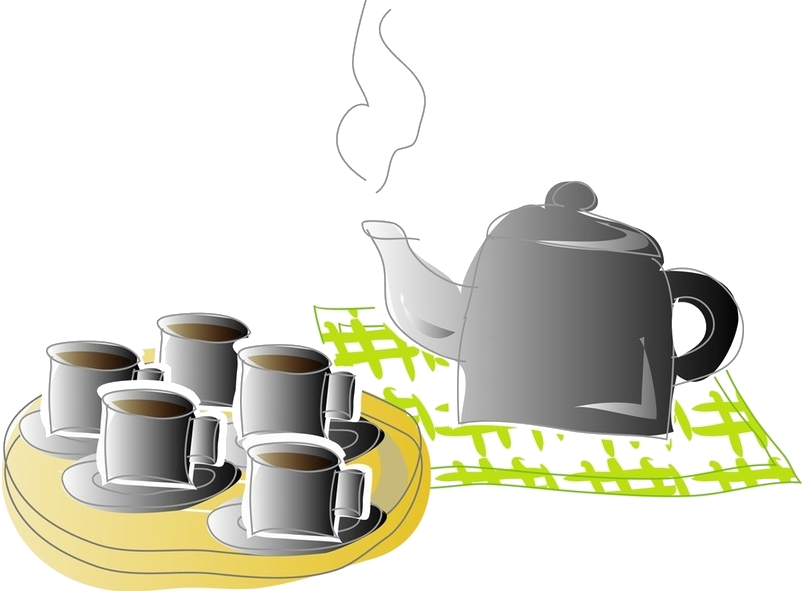
\includegraphics[width=0.75\textwidth]{figure/relax.png}
\end{figure}
\end{frame}

%\section{XML Schema}

\begin{frame}[fragile]{CH4 XML Schema}
\begin{figure}
    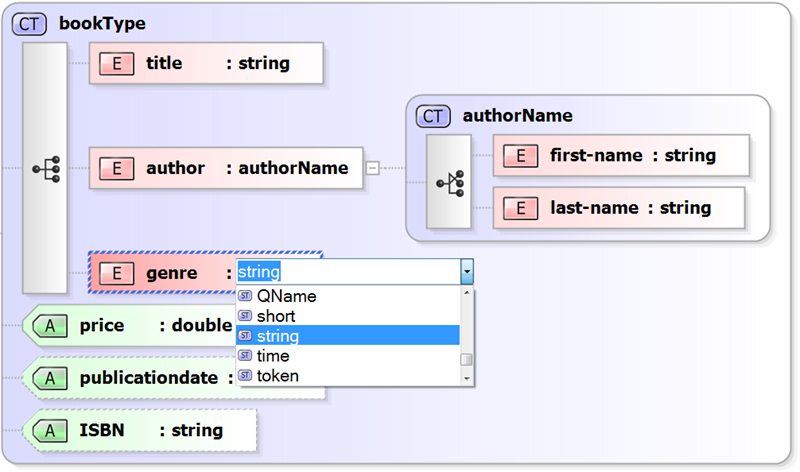
\includegraphics[width=0.9\textwidth]{figure/schema.png}
\end{figure}
\end{frame}

\begin{frame}[fragile]{本章学习目标}
\begin{easylist} \easyitem
& 理解XML Schema的含义及用途
& 掌握XML Schema的元素、属性的作用及使用方式
& 掌握XML Schema的数据类型
& 理解XML Schema的命名空间的概念
\end{easylist}
\end{frame}

\begin{frame}[fragile]{目录}
\begin{easylist} \easyitem
& XML Schema概述
& 快速入门
& 元素声明
& 属性声明
& 数据类型
&& 简单数据类型:SimpleType
&& 复杂数据类型:ComplexType
& XML Schema与命名空间
&& targetNamespace
&& elementFormDefault 与 attributeFormDefault
&& form
& 注释与注解
\end{easylist}
\end{frame}


\subsection{4.1 XML Schema概述}

\begin{frame}[fragile]{4.1 XML Schema概述}
\begin{easylist} \easyitem
& DTD本身存在的不足
&& 具有自己独特的语法,需要特定的解析技术
&& 没有数据类型的概念
&& 不支持命名空间
&& 扩展机制复杂且较为脆弱
& XML Schema是DTD的替代
&& DTD较为简单,二者会长期并存
\end{easylist}
\end{frame}


\subsection{4.2 XML Schema快速入门}

\begin{frame}[fragile]{4.2 XML Schema快速入门}
\begin{shaded}
一个Schema文档由元素、属性、命名空间和XML文档中的其他结点组成,并且至少要包含Schema根元素和XML Schema命名空间定义。
\end{shaded}
\end{frame}


\subsubsection{4.2.1 快速实例}
\begin{frame}[fragile, allowframebreaks]{4.2.1 实例—XML文档}
\begin{lstlisting}[tabsize=8, basicstyle=\small\tt, language=XML]
<?xml version="1.0"?>
<book isbn="7535421016" xmlns:xsi="http://www.w3.org/2001/XMLSchema-instance" 
       xsi:noNamespaceSchemaLocation="4-1.xsd">
    <name>康熙大帝</name>
    <author>二月河</author>
    <price>86</price>
    <pages>2012</pages>    
    <introduction>清顺治十八年,恶疾天花袭击了皇宫,皇帝爱妃
命丧黄泉,顺治痛不欲生,立意遁入空门。危急之际...</introduction>
    <publish>
        <publisher>长江文艺出版社</publisher>
        <pubDate>2006-01-01</pubDate>
    </publish>    
</book>
\end{lstlisting}
\begin{easylist} \easyitem
& 行2中的“xmlns:xsi”属性表示命名空间xsi(XML Schema Instance)为一个XML Schema实例
& 通过xsi:noNamespaceSchemaLocation与指定的XML Schema文件4-1.xsd建立关联,实现有效性验证
\end{easylist}
\end{frame}

\begin{frame}[fragile, allowframebreaks]{实例—Schema文档}
\begin{lstlisting}[tabsize=8, basicstyle=\small\tt, language=XML]
<?xml version="1.0" encoding="UTF-8"?>
<xsd:schema xmlns:xsd="http://www.w3.org/2001/XMLSchema">
    <xsd:element name="book">
        <xsd:complexType>
            <xsd:sequence>
                <xsd:element name="name" type="xsd:string"/>
                <xsd:element name="author" type="xsd:string"/>
                <xsd:element name="price" type="xsd:integer"/>
                <xsd:element name="pages" type="xsd:integer"/>
                <xsd:element name="introduction" type="xsd:string"/>
                <xsd:element name="publish" minOccurs="0" maxOccurs="1">
                    <xsd:complexType>
                        <xsd:sequence>
                            <xsd:element name="publisher" type="xsd:string"/>
                            <xsd:element name="pubDate" type="xsd:date"/>
                        </xsd:sequence>
                    </xsd:complexType>
                </xsd:element>
            </xsd:sequence>
            <xsd:attribute name="isbn" type="xsd:string"/>
        </xsd:complexType>
    </xsd:element>
</xsd:schema>
\end{lstlisting}

\begin{easylist} \easyitem
& 每一个XML Schema文档都以schema作为根元素,并位于命名空间“http://www.w3.org/2001/XMLSchema”之中
& 推荐使用的命名空间前缀有两种常见方式
&&  xsd:XML Schema Document的缩写表示
&& xs:XML Schema的缩写表示
\end{easylist}
\end{frame}


\subsubsection{4.2.2 Schema文档结构}
\begin{frame}[fragile]{4.2.2 Schema文档结构}
\begin{easylist} \easyitem
& Schema文档构成
&& 定义命名空间
&& 定义根元素的名字和类型
&& 定义子元素的名字和类型,并说明和根元素的关系
& 简单Schema文档
\begin{lstlisting}[tabsize=8, basicstyle=\small\tt, language=XML]
<?xml version="1.0" encoding="UTF-8"?>
<xsd:schema xmlns:xsd="http://www.w3.org/2001/XMLSchema">
    <!-- 详细声明内容 -->
</xsd:schema>
\end{lstlisting}
\end{easylist}
\end{frame}


\begin{frame}[fragile]{Schema文档可以树状方式查看}
\begin{figure}
    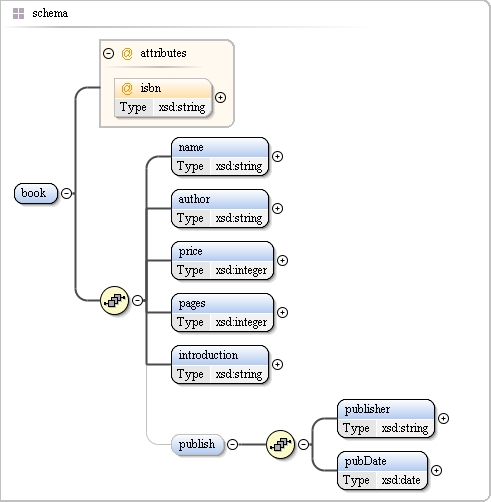
\includegraphics[width=0.75\textwidth]{figure/schema-tree.png}
\end{figure}
\end{frame}


\subsubsection{4.2.3 引用方式}
\begin{frame}[fragile]{4.2.3 引用方式}
\begin{easylist} \easyitem
& 最为常见的引用方式示例:
\begin{lstlisting}[tabsize=8, basicstyle=\small\tt, language=XML]
<book isbn="7535421016" xmlns:xsi="http://www.w3.org/2001/XMLSchema-instance" 
    xsi:noNamespaceSchemaLocation="4-1.xsd">
    <!-- XML文档内容…… -->
</book>
\end{lstlisting}
\end{easylist}
\end{frame}


\subsubsection{4.2.4 包含与导入}
\begin{frame}[fragile]{4.2.4 包含与导入}
\begin{easylist} \easyitem
& 借助于包含(include)或导入(import)机制,一个主模式文档可以由多个模式文档组合而成
&& 当其他模式文档与主模式文档具有相同的目标命名空间时,可以使用包含方式
&& 当各自拥有不同的目标命名空间时,则使用导入方式
& 适用于复杂场景
\end{easylist}
\end{frame}



\subsection{4.3 XML Schema的元素声明}

\begin{frame}[fragile]{4.3 XML Schema的元素声明}
\begin{shaded}
XML Schema通过element语法对元素进行声明,支持元素的类型名称、数据类型以及默认值、固定值等设置,元素可以是简单类型,也可以是复杂类型
\end{shaded}
\end{frame}


\subsubsection{4.3.1 schema根元素}
\begin{frame}[fragile]{4.3.1 schema根元素}
\begin{easylist} \easyitem
&  Schema文档都必须定义一个名称为schema的根元素
&& 该元素包含8个可选的属性,分别为attributeFormDefault、blockDefault、elementFormDefault、finalDefault、id、targetNamespace、version、xml:lang
& 简单示例
\begin{lstlisting}[tabsize=8, basicstyle=\small\tt, language=XML]
<?xml version="1.0" encoding="UTF-8"?>
<xsd:schema id="mySchema" xmlns:xsd="http://www.w3.org/2001/XMLSchema">
    <!-- XML Schema文档的详细定义 -->
</xsd:schema>
\end{lstlisting}
&& 可选的id属性为了方便用户的使用
&& 对应的名称空间为: http://www.w3.org/2001/XMLSchema
\end{easylist}
\end{frame}


\subsubsection{4.3.2 element元素}
\begin{frame}[fragile]{4.3.2 element元素}
\begin{easylist} \easyitem
&  element元素用于声明元素的属性,语法如下:
\begin{lstlisting}[tabsize=8, basicstyle=\small\tt, language=XML, numbers=none]
<xsd:element name="元素名称" type="元素类型"/>
\end{lstlisting}
&& name是元素类型的名称
&& 必选的type属性用于说明元素的数据类型

&  例子
\begin{lstlisting}[tabsize=8, basicstyle=\small\tt, language=XML, numbers=none]
<xsd:element name="title" type="xsd:string"/>
\end{lstlisting}
\end{easylist}
\end{frame}


\subsubsection{4.3.3 elment元素的默认值和固定值}
\begin{frame}[fragile]{4.3.3 elment元素的默认值和固定值}
\begin{easylist} \easyitem
& default属性
\begin{lstlisting}[tabsize=8, basicstyle=\small\tt, language=XML, numbers=none]
<xsd:element name="gender" type="xsd:string" default="男"/>
\end{lstlisting}
&& 当对应元素为空时,填入默认值
&& “空”的定义与数据类型相关
&&& 例如string,本身就允许空值,因此其默认值不会被填充
&&& integer数据类型的空元素会被认为是空的,并将填入默认值
&&& 如果元素的xsi:nil属性被设置为true,也不会插入默认值

& fixed属性
&& 元素值不能被改写,必须与fixed中所指定的值保持等价
&& 等价并不意味形式完全一样
\end{easylist}
\end{frame}


\begin{frame}[fragile]{元素默认值行为举例}
\begin{easylist} \easyitem
& Schema文档
\begin{lstlisting}[tabsize=8, basicstyle=\small\tt, language=XML]
<?xml version="1.0" encoding="UTF-8"?>
<xsd:schema xmlns:xsd="http://www.w3.org/2001/XMLSchema">
    <xsd:element name="name" type="xsd:string"/>
    <xsd:element name="author" type="xsd:string" default="佚名"/>
    <xsd:element name="price" type="xsd:integer" default="20"/>
</xsd:schema>
\end{lstlisting}
\end{easylist}
\end{frame}


\begin{frame}[fragile]{元素默认值行为举例}
\begin{easylist} \easyitem
& 指定值: 前后不变
&& 扩充前: <author>霍金</author>
&& 扩充后: <author>霍金</author>

& 空元素(string): 字符串的默认值不填充
&& 扩充前: <author></author>
&& 扩充后: <author></author>

& 空元素(integer): 整数类型的默认值自动填充
&& 扩充前: <price></price>
&& 扩充后: <price>20</price>

& 元素为空: 保持不变
&& 扩充前: <price xsi:nil="true"/>
&& 扩充后: <price xsi:nil="true"/>
\end{easylist}
\end{frame}



\begin{frame}[fragile]{元素固定值行为举例}
\begin{easylist} \easyitem
& Schema文档
\begin{lstlisting}[tabsize=8, basicstyle=\small\tt, language=XML, numbers=none]
<xsd:element name="count" type="xsd:integer" fixed="10"/>
\end{lstlisting}
& 有效实例
\begin{lstlisting}[tabsize=8, basicstyle=\small\tt, language=XML]
    <count>10</count>
    <count>010</count>
    <count>+10</count>
    <count></count>
    <count/>
\end{lstlisting}
\end{easylist}
\end{frame}



\subsubsection{4.3.4 元素的引用和替代}
\begin{frame}[fragile]{4.3.4 元素的引用和替代}
\begin{easylist} \easyitem
& 目的
&& 通过全局元素声明和元素引用,利用ref属性与已定义的元素进行关联
&& 避免重复定义
&& 如下例中的第20行和27行
\end{easylist}
\end{frame}


\begin{frame}[fragile, allowframebreaks]{示例文档}
\begin{lstlisting}[tabsize=8, basicstyle=\small\tt, language=XML]
<?xml version="1.0" encoding="UTF-8"?>
<xsd:schema xmlns:xsd="http://www.w3.org/2001/XMLSchema">
    <xsd:element name="book">
        <xsd:complexType>
            <xsd:sequence>
                <xsd:element name="name" type="xsd:string"/>
                <xsd:element name="author" type="xsd:string"/>
                <xsd:element name="price" type="xsd:decimal"/>
                <xsd:element name="introduction" type="xsd:string"/>
            </xsd:sequence>
        </xsd:complexType>
    </xsd:element>
    
    <xsd:element name="books">
        <xsd:complexType>
            <xsd:sequence>
                <xsd:element name="computer-books">
                    <xsd:complexType>
                        <xsd:sequence>
                            <xsd:element ref="book" maxOccurs="10"/>
                        </xsd:sequence>
                    </xsd:complexType>
                </xsd:element>
                <xsd:element name="math-books">
                    <xsd:complexType>
                        <xsd:sequence>
                            <xsd:element ref="book" maxOccurs="10"/>
                        </xsd:sequence>
                    </xsd:complexType>
                </xsd:element>
            </xsd:sequence>
        </xsd:complexType>
    </xsd:element>
</xsd:schema>
\end{lstlisting}
\end{frame}



\subsection{4.4 XML Schema的属性声明}

\begin{frame}[fragile]{4.4 XML Schema的属性声明}
\begin{easylist} \easyitem
& 通过attribute元素进行属性声明
& 属性声明与元素声明的区别
&& 属性的类型只能是简单类型
&& 属性不能包含子属性,而元素可以包含子元素
&& 属性之间没有顺序要求
\end{easylist}
\end{frame}


\subsubsection{4.4.1 属性声明}
\begin{frame}[fragile]{4.4.1 属性声明}
\begin{easylist} \easyitem
&  语法形式:
\begin{lstlisting}[tabsize=8, basicstyle=\small\tt, language=XML, numbers=none]
<xsd:attribute name="属性名称" type="属性类型"/>
\end{lstlisting}
& Example:
\begin{lstlisting}[tabsize=8, basicstyle=\small\tt, language=XML, numbers=none]
<xsd:attribute name="类别" type="xsd:string"/>
\end{lstlisting}
& 支持全局属性声明和属性引用,以提高复用程度
\end{easylist}
\end{frame}


\begin{frame}[fragile]{use属性}
\begin{easylist} \easyitem
&  use属性用于指示所声明的属性是否在XML文档中必须出现
& 取值:
&& optional:
&&& 可选属性,所声明的属性可以出现,也可以不出现,为use属性的默认值。
&& required
&&& 该属性必须指定,不能缺省。
&& prohibited
&&& 禁止在元素上使用该属性,等同于把该属性删除掉。
\end{easylist}
\end{frame}


\begin{frame}[fragile]{例子}
\begin{lstlisting}[tabsize=8, basicstyle=\small\tt, language=XML]
<?xml version="1.0" encoding="UTF-8"?>
<xsd:schema xmlns:xsd="http://www.w3.org/2001/XMLSchema">
    <xsd:attribute name="code" type="xsd:string"/>
    
    <xsd:element name="course">
        <xsd:complexType>
            <xsd:sequence>
                <xsd:element name="title" type="xsd:string"/>
                <xsd:element name="teacher" type="xsd:string"/>
            </xsd:sequence>
            <xsd:attribute ref="code" use="required"/>
            <xsd:attribute name="location" type="xsd:string" use="prohibited"/>
        </xsd:complexType>
    </xsd:element>
</xsd:schema>
\end{lstlisting}
\end{frame}


\subsubsection{4.4.2 指派属性类型}
\begin{frame}[fragile]{4.4.2 指派属性类型}
\begin{easylist} \easyitem
&  属性不能包含子元素和属性,一定是简单类型,指定方式:
&& 在属性声明中通过type属性指定为简单类型
&& 通过simpleType以匿名类型的方式为属性指定类型
&& 不明确指定属性的类型,
&&& 此时属性的类型为anySimpleType,可以是任意合法的属性取值
\end{easylist}
\end{frame}


\begin{frame}[fragile, allowframebreaks]{例子}
\begin{lstlisting}[tabsize=8, basicstyle=\small\tt, language=XML]
<?xml version="1.0" encoding="UTF-8"?>
<xsd:schema xmlns:xsd="http://www.w3.org/2001/XMLSchema">
    <xsd:attribute name="code" type="xsd:string"/>
    <xsd:attribute name="classroom"/>
    <xsd:attribute name="category">
        <xsd:simpleType>
            <xsd:restriction base="xsd:string">
                <xsd:enumeration value="专业选修"/>
                <xsd:enumeration value="专业必修"/>
            </xsd:restriction>
        </xsd:simpleType>
    </xsd:attribute>
</xsd:schema>
\end{lstlisting}
\begin{easylist} \easyitem
& 行4~11以simpleType匿名方式声明category属性
& 行12的classroom的属性类型取默认值anySimpleType
\end{easylist}
\end{frame}


\subsubsection{4.4.3 属性的默认值和固定值}
\begin{frame}[fragile]{4.4.3 属性的默认值和固定值}
\begin{easylist} \easyitem
& 默认值和固定值分别通过default和fixed属性进行设置
&& 二者不能同时出现,定义和扩充的方式与element元素中的方式一致
&& 指定了默认值的属性在XML实例中没有出现,则该属性及其默认值会被填入
&& 指定了固定值的属性,如果在XML实例中出现,所指定的属性值应和Schema中定义的固定值相等,如未指定,则该属性及其固定值会被自动填入
\end{easylist}
\end{frame}


\begin{frame}[fragile, allowframebreaks]{例子}
\begin{lstlisting}[tabsize=8, basicstyle=\small\tt, language=XML]
<?xml version="1.0" encoding="UTF-8"?>
<xsd:schema xmlns:xsd="http://www.w3.org/2001/XMLSchema">
    <xsd:element name="course">
        <xsd:complexType>
            <xsd:sequence>
                <xsd:element name="title" type="xsd:string"/>
            </xsd:sequence>
            <xsd:attribute name="periods" type="xsd:integer" default="3"/>
            <xsd:attribute name="location" type="xsd:string" fixed="ROOM-403"/>
        </xsd:complexType>
    </xsd:element>
</xsd:schema>
\end{lstlisting}

\newpage
\begin{lstlisting}[tabsize=8, basicstyle=\small\tt, language=XML]
<?xml version="1.0" encoding="UTF-8"?>
<course xmlns:xsi="http://www.w3.org/2001/XMLSchema-instance" 
    xsi:noNamespaceSchemaLocation="4-7.xsd" periods="4">
    <title>XML原理与应用</title>
</course>
\end{lstlisting}
\end{frame}



\subsection{4.5 XML Schema的数据类型}
\begin{frame}[fragile]{4.5 XML Schema的数据类型}
\begin{easylist} \easyitem
& 简单类型
&& 内置的简单数据类型
&& 用户通过simpleType自定义的简单数据类型
& 复杂类型
&& 通过complexType进行定义
\end{easylist}
\end{frame}


\subsubsection{4.5.1 简单数据类型:SimpleType}
\begin{frame}[fragile]{4.5.1 简单数据类型:SimpleType}
\begin{easylist} \easyitem
& 原子类型
&& 内置数据类型
&&& 原始数据类型(Primitive)
&&& 派生数据类型(Derived)
&& 自定义简单类型
& 列表类型
& 联合类型
\end{easylist}
\end{frame}


\begin{frame}[fragile]{4.5.1.1 内置简单类型}
\begin{easylist} \easyitem
& 内置数据类型可以用来描述元素的内容和属性取值,或者组合生成其他自定义数据类型。
& 包括原始数据类型(Primitive)和派生数据类型(Derived)两类
\end{easylist}
\end{frame}


\begin{frame}[fragile]{常用的原始数据类型}
\begin{table}[!hbp] 
\begin{tabular}{|l|l|}
\Xhline{1.3pt}
类型 & 描述 \\ \Xhline{1.3pt}
string & 字符串\\ \hline
boolean & 代表真假的布尔值\\ \hline
decimal & 十进制数字\\ \hline
float & 32位单精度浮点数\\ \hline
double & 64位双精度浮点数\\ \hline
date & 阳历日期\\ \hline
time & 每天中任何一个时刻,如18:36:16\\ \hline
dateTime& 阳历日期和某一天时间组合而成的某个时刻\\ \hline
\end{tabular}
\end{table}
\end{frame}


\begin{frame}[fragile]{常用的派生数据类型}
\begin{table}[!hbp] 
\begin{tabular}{|l|l|}
\Xhline{1.3pt}
类型 & 描述 \\ \Xhline{1.3pt}
integer & 任意长度的整数类型 \\ \hline
long & 64位有符号整数 \\ \hline
int & 32位有符号整数 \\ \hline
byte & 8位有符号整数 \\ \hline
unsignedInt & 32位无符号整数 \\ \hline
negativeInteger & 任意长度的负整数类型 \\ \hline
nonNegativeInteger & 大于等于零的整数 \\ \hline
normalizedString & 将回车、换行、制表符已转为空格 \\ \hline
\end{tabular}
\end{table}
\end{frame}


\begin{frame}[fragile]{XML Schema内置数据类型的层次结构}
\begin{figure}
    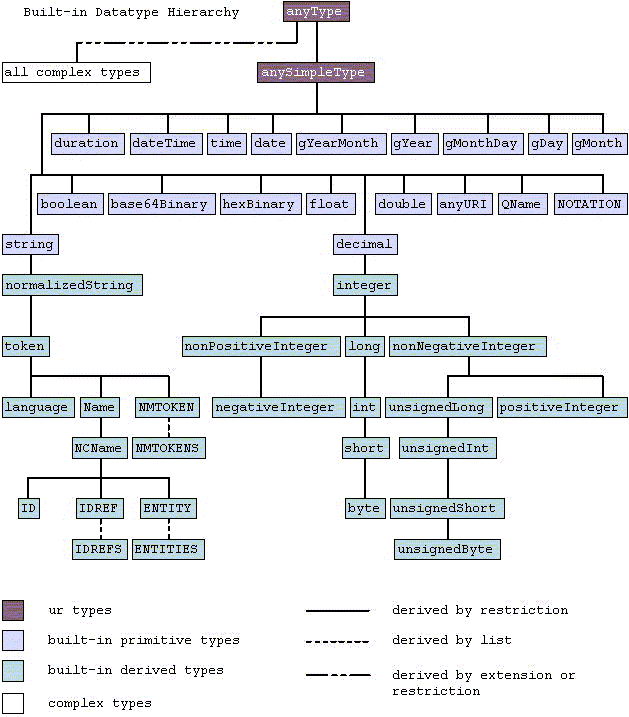
\includegraphics[width=0.75\textwidth]{figure/schema-type-hierarchy.png}
\end{figure}
\end{frame}


\begin{frame}[fragile]{4.5.1.2 自定义简单类型}
\begin{easylist} \easyitem
& 根据已经存在的简单数据类型通过simpleType关键字进行定义
& 总是通过对一个已有简单类型进行约束(restriction)派生出来
& 用户自定义的简单数据类型语法:
\begin{lstlisting}[tabsize=8, basicstyle=\small\tt, language=XML, numbers=none]
<xsd:simpleType name="自定义数据类型的名称">
    <xsd:restriction base="所基于的简单数据类型的名称">
        <!-- 约束面 -->
    </xsd:restriction>
</xsd:simpleType>
\end{lstlisting}
&& 自定义简单类型通过restriction元素对现有类型进行约束
&& 约束面
\end{easylist}
\end{frame}


\begin{frame}[fragile]{simpleType的约束面}
\begin{table}[!hbp] 
\begin{tabular}{|l|l|}
\Xhline{1.3pt}
属性 & 描述 \\ \Xhline{1.3pt}
pattern & 采用正则表达式方式限定数据的显示格式 \\ \hline
enumeration & 限定用户的取值为指定的数据集合 \\ \hline
length & 指定数据的长度 \\ \hline
maxExclusive & 指定数据的最大值(取值小于该指定值) \\ \hline
maxInclusive & 指定数据的最大值(取值小于或等于该指定值) \\ \hline
maxLength & 指定长度的最大值 \\ \hline
minExclusive & 指定数据的最小值(取值大于该指定值) \\ \hline
minInclusive & 指定数据的最小值(取值大于或等于该指定值) \\ \hline
minLength & 指定最小长度 \\ \hline
whiteSpace & 决定应用程序如何处理元素内容中的空白符 \\ \hline
totalDigits & 限定数字的最多位数 \\ \hline
fractionDigits & 限定最大的小数位,用于控制精度 \\ \hline
\end{tabular}
\end{table}
\end{frame}


\begin{frame}[fragile]{示例}
\begin{shaded}
<mobile>13800138000</ mobile >是描述一个手机号码的XML片段,此标记中的内容必须为数字,长度为固定的11位
\end{shaded}

\begin{lstlisting}[tabsize=8, basicstyle=\small\tt, language=XML]
<xsd:simpleType name="mobileType">
    <xsd:restriction base="xsd:string">
        <xsd:length value="11"/>
        <xsd:pattern value="\d{11}"/>
    </xsd:restriction>
</xsd:simpleType>
\end{lstlisting}
\end{frame}


\begin{frame}[fragile]{练习}
\begin{easylist} \easyitem
& 定义一个整数,其取值范围为[10, 100]
& 定义一个字符串,最少由4个字符组成,最多由16个字符组成
& 定义一个性别类型,其取值只能为“男”或“女”
\end{easylist}
\end{frame}


\begin{frame}[fragile]{4.5.1.3 列表类型与联合类型}
\begin{easylist} \easyitem
& 列表类型所定义的元素或属性的值可以包含多个原子值,这些并列的原子值之间通过空格分隔。列表元素使用list元素进行定义
& 语法:
\begin{lstlisting}[tabsize=8, basicstyle=\small\tt, language=XML, numbers=none]
<xsd:simpleType name="列表类型名">
    <xsd:list itemType="某一原子类型"/>
</xsd:simpleType>
\end{lstlisting}
\end{easylist}
\end{frame}


\begin{frame}[fragile]{列表类型示例}
\begin{lstlisting}[tabsize=8, basicstyle=\small\tt, language=XML]
<xsd:element name="years" type="yearListType"/>
<xsd:simpleType name="yearType">
    <xsd:restriction base="xsd:string">
        <xsd:pattern value="\d{4}"/>
    </xsd:restriction>
</xsd:simpleType>
<xsd:simpleType name="yearListType">
    <xsd:list itemType="yearType"/>
</xsd:simpleType>
\end{lstlisting}

\begin{lstlisting}[tabsize=8, basicstyle=\small\tt, language=XML, numbers=none]
<years>2010 2011 2012</years>
\end{lstlisting}
\end{frame}


\begin{frame}[fragile]{联合类型}
\begin{easylist} \easyitem
& 语法:
\begin{lstlisting}[tabsize=8, basicstyle=\small\tt, language=XML, numbers=none]
<xsd:simpleType name="联合类型名">
<xsd:union memberTypes="简单类型1 简单类型2 ……"/>
</xsd:simpleType>
\end{lstlisting}
&& 联合类型可以包含多个简单类型,所包含的简单类型既可以是原子类型,也可以是列表类型
&& 取值可以是memberTypes属性值中所指明的某一个简单类型的实例
\end{easylist}
\end{frame}


\begin{frame}[fragile]{联合类型示例}
\begin{lstlisting}[tabsize=8, basicstyle=\small\tt, language=XML]
<xsd:element name="whichYear" type="yearUnionType"/>
<xsd:simpleType name="yearUnionType">
    <xsd:union memberTypes="xsd:date yearListType"/>
</xsd:simpleType>
\end{lstlisting}

\par 正确用例:
\begin{lstlisting}[tabsize=8, basicstyle=\small\tt, language=XML]
<whichYear>2008-02-09</whichYear>
<whichYear>2010</whichYear>
\end{lstlisting}

\par 错误用例:
\begin{lstlisting}[tabsize=8, basicstyle=\small\tt, language=XML]
<whichYear>2008-02-09 2010</whichYear>
<whichYear>2010年</whichYear>
\end{lstlisting}
\end{frame}


\subsubsection{4.5.2 复杂数据类型:ComplexType}
\begin{frame}[fragile]{4.5.2 复杂数据类型:ComplexType}
\begin{easylist} \easyitem
& 四种复杂数据类型
&& 只包含文本的简单内容类型
&& 只包含子元素的纯元素内容类型
&& 包含子元素和文本的混合内容类型
&& 空元素
\end{easylist}
\end{frame}


\begin{frame}[fragile]{复杂数据类型的基本语法形式}
\begin{lstlisting}[tabsize=8, basicstyle=\small\tt, language=XML, numbers=none]
<xsd:complexType name="名称" id=ID mixed=BOOLEAN: false>
    <xsd:annotation | simpleContent | complexContent | group | all | choice | sequence | attribute | attributeGroup | anyAttribute>...
</xsd:complexType>
\end{lstlisting}
\begin{easylist} \easyitem
& name 复杂类型的名称
& id 该元素的ID,可选项
& mixed,可选布尔类型,该复杂类型的子元素之中是否允许出现字符数据,默认值为false
\end{easylist}
\end{frame}


\begin{frame}[fragile]{复杂类型的内容模型}
\begin{easylist} \easyitem
& 复杂类型的内容模型指复杂类型子元素的顺序和结构称
&& 内容模型不依赖于属性,但允许有属性
&& complexType下可以创建的内容模型有
&&& simpleContent、complexContent、sequence、group、all、choice、annotation
\end{easylist}
\end{frame}


\begin{frame}[fragile]{4.5.2.1 simpleContent}
\begin{easylist} \easyitem
& 用于从简单类型派生复杂类型
& 适用于元素包含字符内容和属性但不包含子元素的情况
& 简单内容模型的复杂类型可以包含属性,而简单类型不可
& 语法:
\begin{lstlisting}[tabsize=8, basicstyle=\small\tt, language=XML, numbers=none]
<xsd:simpleContent id=ID >
    <xsd:annotation | restriction | extension>...
</xsd:simpleContent>
\end{lstlisting}
\end{easylist}
\end{frame}


\begin{frame}[fragile, allowframebreaks]{simpleContent示例}
\begin{lstlisting}[tabsize=8, basicstyle=\small\tt, language=XML]
<?xml version="1.0" encoding="UTF-8"?>
<xsd:schema xmlns:xsd="http://www.w3.org/2001/XMLSchema">
    <xsd:element name="book">
        <xsd:complexType>
            <xsd:simpleContent>
                <xsd:extension base="xsd:string">
                    <xsd:attribute name="isbn" type="xsd:string" use="required"/>
                </xsd:extension>
            </xsd:simpleContent>
        </xsd:complexType>
    </xsd:element>
</xsd:schema>
\end{lstlisting}

\newpage
\begin{lstlisting}[tabsize=8, basicstyle=\small\tt, language=XML]
<?xml version="1.0" encoding="UTF-8"?>
<book xmlns:xsi="http://www.w3.org/2001/XMLSchema-instance"
      xsi:noNamespaceSchemaLocation="4-8.1.xsd"
      isbn="6-666-66666-6">
      XML原理与应用
</book>
\end{lstlisting}
\end{frame}


\begin{frame}[fragile]{4.5.2.2 complexContent}
\begin{easylist} \easyitem
& 用于对复杂数据类型进行扩展或限制,从复杂类型派生新的复杂类型
& 语法:
\begin{lstlisting}[tabsize=8, basicstyle=\small\tt, language=XML, numbers=none]
<xsd:complexContent id=ID mixed=true|false>
    <xsd:annotation | restriction | extension>...
</xsd:simpleContent>
\end{lstlisting}
\end{easylist}
\end{frame}


\begin{frame}[fragile, allowframebreaks]{complexContent示例}
\begin{lstlisting}[tabsize=8, basicstyle=\small\tt, language=XML]
<?xml version="1.0" encoding="UTF-8"?>
<xsd:schema xmlns:xsd="http://www.w3.org/2001/XMLSchema">
    <xsd:element name="student" type="studentType"/>

    <xsd:complexType name="personType">
        <xsd:sequence>
            <xsd:element name="name" type="xsd:string"/>
            <xsd:element name="age" type="xsd:integer"/>
        </xsd:sequence>
    </xsd:complexType>
    
    <xsd:complexType name="studentType">
        <xsd:complexContent>
            <xsd:extension base="personType">
                <xsd:sequence>
                    <xsd:element name="class" type="xsd:string"/>
                    <xsd:element name="major" type="xsd:string"/>
                </xsd:sequence>
            </xsd:extension>
        </xsd:complexContent>
    </xsd:complexType>
</xsd:schema>
\end{lstlisting}
\end{frame}


\begin{frame}[fragile]{4.5.2.3 顺序声明:sequence}
\begin{easylist} \easyitem
& 最为常用的内容模型定义方式
& 用于限定sequence内部的一组元素的出现顺序
& 带有minOccurs和maxOccurs两个属性,作用于整个顺序组合
\end{easylist}
\end{frame}


\begin{frame}[fragile, allowframebreaks]{sequence示例}
\begin{lstlisting}[tabsize=8, basicstyle=\small\tt, language=XML]
<?xml version="1.0" encoding="UTF-8"?>
<xsd:schema xmlns:xsd="http://www.w3.org/2001/XMLSchema">
    <xsd:element name="person" type="personType"/>
    <xsd:complexType name="personType">
        <xsd:sequence minOccurs="1" maxOccurs="10">
            <xsd:element name="name" type="xsd:string"/>
            <xsd:element name="age" type="xsd:integer"/>
        </xsd:sequence>
    </xsd:complexType>
</xsd:schema>
\end{lstlisting}

\newpage
\par 以下代码片段能够通过有效性验证?
\begin{lstlisting}[tabsize=8, basicstyle=\small\tt, language=XML]
<name>刘备</name>
<age>35</age>
<name>张飞</name>
<age>35</age>
\end{lstlisting}

\par 以下代码片段能够通过有效性验证?
\begin{lstlisting}[tabsize=8, basicstyle=\small\tt, language=XML]
<age>35</age>
<name>刘备</name>
\end{lstlisting}
\end{frame}


\begin{frame}[fragile]{4.5.2.4 选择声明:choice}
\begin{easylist} \easyitem
& 多选一
\end{easylist}

\begin{lstlisting}[tabsize=8, basicstyle=\small\tt, language=XML]
<?xml version="1.0" encoding="UTF-8"?>
<xsd:schema xmlns:xsd="http://www.w3.org/2001/XMLSchema">
    <xsd:complexType name="personType">
        <xsd:sequence minOccurs="1" maxOccurs="10">
            <xsd:element name="name" type="xsd:string"/>
            <xsd:element name="age" type="xsd:integer"/>
            <xsd:choice>
                <xsd:element name="wife" type="xsd:string"/>
                <xsd:element name="husband" type="xsd:string"/>
            </xsd:choice>
        </xsd:sequence>
    </xsd:complexType>
</xsd:schema>
\end{lstlisting}
\end{frame}



\begin{frame}[fragile]{4.5.2.5 分组声明:group}
\begin{easylist} \easyitem
& 使用方式
&& group声明
&&& 用于指定一个模型组的定义,定义该分组内包含的内容,并以schema元素的子元素形式出现;
&& group引用
&&& 对已经定义分组进行引用,此时group出现在复杂类型定义或其他模型组定义的内部。
\end{easylist}
\end{frame}

\begin{frame}[fragile, allowframebreaks]{group示例}
\begin{lstlisting}[tabsize=8, basicstyle=\small\tt, language=XML]
<?xml version="1.0" encoding="UTF-8"?>
<xsd:schema xmlns:xsd="http://www.w3.org/2001/XMLSchema">
    <xsd:group name="HeightAndWeightGroup">
        <xsd:sequence>
            <xsd:element name="height" type="xsd:integer"/>
            <xsd:element name="weight" type="xsd:integer"/>
        </xsd:sequence>
    </xsd:group>
    
    <xsd:complexType name="personType">
        <xsd:sequence minOccurs="1" maxOccurs="10">
            <xsd:element name="name" type="xsd:string"/>
            <xsd:element name="age" type="xsd:integer"/>
            <xsd:choice>
                <xsd:element name="wife" type="xsd:string"/>
                <xsd:element name="husband" type="xsd:string"/>
            </xsd:choice>
            <xsd:group ref="HeightAndWeightGroup"/>
        </xsd:sequence>
    </xsd:complexType>
</xsd:schema>
\end{lstlisting}
\end{frame}


\begin{frame}[fragile]{4.5.2.6 ALL声明:all}
\begin{easylist} \easyitem
& 元素可以在实例文档中以任意顺序出现
&& all元素的任何子元素声明,其minOccurs属性只能取0或1的值,maxOccurs属性只能取1值
& all示例:
\begin{lstlisting}[tabsize=8, basicstyle=\small\tt, language=XML]
<?xml version="1.0" encoding="UTF-8"?>
<xsd:schema xmlns:xsd="http://www.w3.org/2001/XMLSchema">
    <xsd:complexType name="personType">
        <xsd:all>
            <xsd:element name="name" type="xsd:string"/>
            <xsd:element name="age" type="xsd:integer"/>
        </xsd:all>
    </xsd:complexType>
</xsd:schema>
\end{lstlisting}
\end{easylist}
\end{frame}


\begin{frame}[fragile, allowframebreaks]{all示例 }
\begin{lstlisting}[tabsize=8, basicstyle=\small\tt, language=XML]
<?xml version="1.0" encoding="UTF-8"?>
<xsd:schema xmlns:xsd="http://www.w3.org/2001/XMLSchema">
    <xsd:group name="HeightAndWeightGroup">
        <xsd:sequence>
            <xsd:element name="height" type="xsd:integer"/>
            <xsd:element name="weight" type="xsd:integer"/>
        </xsd:sequence>
    </xsd:group>
    
    <xsd:complexType name="personType">
        <xsd:sequence minOccurs="1" maxOccurs="10">
            <xsd:element name="name" type="xsd:string"/>
            <xsd:element name="age" type="xsd:integer"/>
            <xsd:choice>
                <xsd:element name="wife" type="xsd:string"/>
                <xsd:element name="husband" type="xsd:string"/>
            </xsd:choice>
            <xsd:group ref="HeightAndWeightGroup"/>
        </xsd:sequence>
    </xsd:complexType>
</xsd:schema>
\end{lstlisting}
\par 该定义方式与上一定义方式的约束效果相同。
\end{frame}



\subsection{4.6 XML Schema与命名空间}
\begin{frame}[fragile]{4.6 XML Schema与命名空间}
\begin{easylist} \easyitem
& targetNamespace
& elementFormDefault
& attributeFormDefault
\end{easylist}
\end{frame}


\subsubsection{4.6.1 targetNamespace}

\begin{frame}[fragile]{4.6.1 targetNamespace}
\begin{easylist} \easyitem
& 每一个Schema文档都可有一个命名空间,称为模式文档的目标命名空间(Target Namespace)
& 每个被全局声明所定义的元素、属性、类型或分组,都与该目标命名空间有关。
& 通过targetNamespace指定所定义元素或属性所隶属的命名空间,
&& 默认情况下仅对全局声明的元素和属性起作用(未设置elementFormDefault和attributeFormDefault)
\end{easylist}
\end{frame}


\begin{frame}[fragile]{targetNamespace示例:4-14.xsd }
\begin{lstlisting}[tabsize=8, basicstyle=\small\tt, language=XML]
<?xml version="1.0" encoding="UTF-8"?>
<xsd:schema xmlns:xsd="http://www.w3.org/2001/XMLSchema"
            targetNamespace="http://www.example.org/test">
    <xsd:element name="course">
        <xsd:complexType>
            <xsd:sequence>
                <xsd:element name="name" type="xsd:string"/>
                <xsd:element name="teacher" type="xsd:string"/>
            </xsd:sequence>
            <xsd:attribute name="code" type="xsd:string" use="required"/>
        </xsd:complexType>
    </xsd:element>
</xsd:schema>
\end{lstlisting}
\end{frame}


\begin{frame}[fragile]{targetNamespace示例:4-14.xml }
\begin{lstlisting}[tabsize=8, basicstyle=\small\tt, language=XML]
<?xml version="1.0" encoding="UTF-8"?>
<test:course xmlns:test=http://www.example.org/test
      xmlns:xsi=http://www.w3.org/2001/XMLSchema-instance
      xsi:schemaLocation="http://www.example.org/test 4-14.xsd" code="106">
    <name>数据挖掘</name>
    <teacher>夏天</teacher>
</test:course>
\end{lstlisting}
\end{frame}


\subsubsection{4.6.2 elementFormDefault与attributeFormDefault}

\begin{frame}[fragile]{4.6.2 elementFormDefault与attributeFormDefault}
\begin{easylist} \easyitem
& elementFormDefault
&& unqualified(默认值)
&&& 内部元素不受目标命名空间的约束
&& qualified
&&& 内部元素也将受到目标命名空间的约束
& attributeFormDefault
&& unqualified(默认值)
&&&  内部自定义的属性不受目标命名空间的约束
&& qualified
&&& 受目标命名空间约束
\end{easylist}
\end{frame}


\subsubsection{4.6.3 form属性}

\begin{frame}[fragile]{4.6.3 form属性}
\begin{easylist} \easyitem
& 如需要对特定元素或属性设置不同于全局的配置,可以借助于element或attribute元素的form属性
& form属性的取值和作用与全局的elementFormDefault或attributeFormDefault相似,但只作用于当前声明的对象。
\end{easylist}
\end{frame}



\subsection{4.7 XML Schema的注释与注解}
\begin{frame}[fragile]{4.7 XML Schema的注释与注解}
\begin{easylist} \easyitem
& 注释:
&& 可以在模式文档中任意插入XML注释,只要符合XML的语法规定即可
& annotation
&& 增强模式文档的机器可读性
&& 不仅提供文档信息,还提供程序信息,允许模式文档使用读者可以理解和机器可以识别的信息来注释
&& 语法:
\begin{lstlisting}[tabsize=8, basicstyle=\small\tt, language=XML, numbers=none]
<xsd:annotation id=ID >
    <xsd:appinfo | documentation>...
</xsd:annotation>
\end{lstlisting}
\end{easylist}
\end{frame}


\begin{frame}[fragile, allowframebreaks]{注解应用示例 }
\begin{lstlisting}[tabsize=8, basicstyle=\small\tt, language=XML]
<?xml version="1.0" encoding="UTF-8"?>
<xsd:schema xmlns:xsd="http://www.w3.org/2001/XMLSchema">
    <xsd:element name="course" type="courseType"/>
    
    <xsd:annotation>
        <xsd:appinfo source="4-18.html"/>
        <xsd:documentation xmlns:html="http://www.w3.org/1999/xhtml">
            <html:p>注解使用示例,下面所声明的<html:strong>courseType</html:strong>自定义复杂类型,为课程类型,包含两个子元素和一个属性。</html:p>
        </xsd:documentation>
    </xsd:annotation>
    <xsd:complexType name="courseType">
        <xsd:sequence>
            <xsd:element name="name" type="xsd:string"/>
            <xsd:element name="teacher" type="xsd:string" form="unqualified"/>
        </xsd:sequence>
        <xsd:attribute name="code" type="xsd:string" form="qualified" use="required">
            <xsd:annotation>
                <xsd:documentation>必须有课程代号属性code</xsd:documentation>
            </xsd:annotation>
        </xsd:attribute>
    </xsd:complexType>
</xsd:schema>
\end{lstlisting}
\end{frame}


\begin{frame}
\begin{center}
    \Huge END
\end{center}
\begin{figure}
    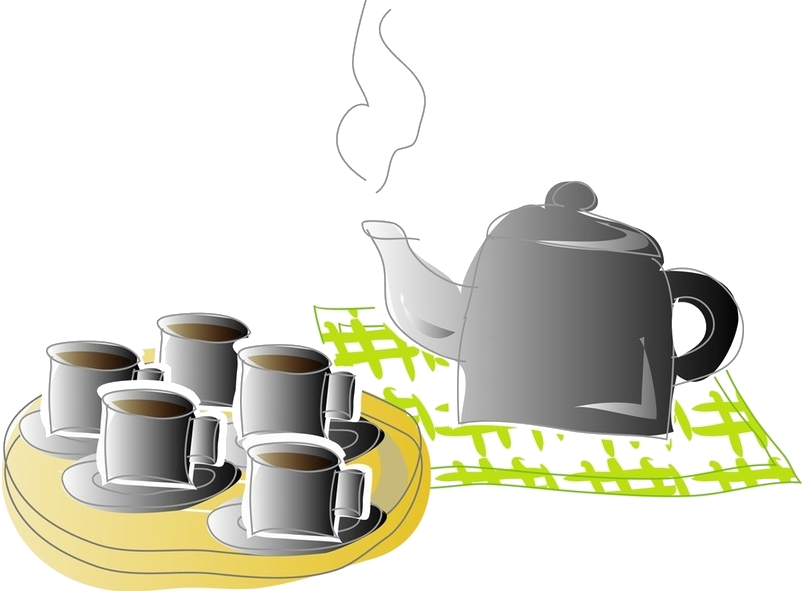
\includegraphics[width=0.75\textwidth]{figure/relax.png}
\end{figure}
\end{frame}


%\section{利用CSS格式化XML}

\begin{frame}[fragile]{CH5 利用CSS格式化XML}
\begin{figure}
    
\includegraphics[width=0.5\textwidth]{figure/css.png}
\end{figure}
\end{frame}

\begin{frame}[fragile]{本章学习目标}
\begin{easylist} \easyitem
& 掌握CSS与XML、HTML的关联方式
& 掌握CSS的常见选择器,理解CSS的属性继承与覆盖原则
& 掌握CSS的颜色、字体和文本属性以及CSS的盒状模型
\end{easylist}
\end{frame}

\begin{frame}[fragile]{目录}
\begin{easylist} \easyitem
& 什么是CSS
& 关联CSS的方法
& CSS语法基础
&& CSS基本语法
&& CSS选择器
&& 继承与覆盖
& CSS重要属性
&& 颜色属性
&& 字体属性
&& 文本属性
&& 盒状模型相关属性
&& 可视格式化模型相关属性
\end{easylist}
\end{frame}


\subsection{5.1 什么是CSS}

\begin{frame}[fragile]{5.1 什么是CSS}
\begin{shaded}
CSS(Cascading Style Sheets),又称为层叠样式表或级联样式表,可以实现对页面布局、字体、颜色、背景和其他图文效果的精准控制,在XML和HTML的呈现中得到了广泛使用。
\end{shaded}

\begin{easylist} \easyitem
& CSS的优点
& CSS的发展历史
&& CSS1
&& CSS2, CSS 2.1
&& CSS 3
\end{easylist}
\end{frame}


\subsection{5.2 关联CSS的方法}

\begin{frame}[fragile]{5.2 关联CSS的方法}
\begin{easylist} \easyitem
& 与传统网页的关联方式
& \em{与XML的关联方式}
\end{easylist}
\end{frame}


\subsubsection{5.2.1 CSS与传统网页的关联方式}
\begin{frame}[fragile]{5.2.1 CSS与传统网页的关联方式}
\begin{easylist} \easyitem
& 独立引用方式
&& 通过HTML中的link标记链接外部独立的样式表文件。
& 网页内嵌方式
&& 在HTML的style标记对中嵌入样式代码块。
& 元素内联方式
&& 在HTML的一般元素上采用style属性直接设置元素的样式信息
\end{easylist}
\end{frame}


\begin{frame}[fragile, allowframebreaks]{示例}
\begin{lstlisting}[tabsize=8, basicstyle=\small\tt, language=HTML, caption=5-1.html]
<html>
    <head>
        <title>CSS DEMO</title>
        <meta http-equiv="Content-Type" content="text/html;charset=utf-8"/>
        <link rel="stylesheet" type="text/css" href="5-1.css"/>
        <style type="text/css">
            h1 {font-size:14pt;font-family:"Microsoft Yahie" 微软雅黑;}
        </style>
    </head>
    <body>
        <h1>图书列表</h1>
        <table>
            <tr>
                <td>ISBN</td><td>名称</td><td>出版社</td><td>价格</td>
            </tr>
            <tr>
                <td>978-7-115-21703-5</td>
                <td style="font-weight:bold;">Python高级编程</td>
                <td>人民邮电出版社</td>
                <td>45.00</td>
            </tr>
            <tr>
                <td>978-7-115-28282-8</td>
                <td>数学之美</td>
                <td>人民邮电出版社</td>
                <td>45.00</td>
            </tr>
            <tr>
                <td>978-7-5641-1139-7</td>
                <td>集体智慧编程(影印版)</td>
                <td>东南大学出版社</td>
                <td>58.00</td>
            </tr>
        </table>
    </body>
</html>
\end{lstlisting}

\begin{lstlisting}[tabsize=8, basicstyle=\small\tt, language=CSS,  caption=5-1.css]
td {
    border:1px solid blue;
}
\end{lstlisting}
\end{frame}


\begin{frame}[fragile]{示例}
\begin{figure}
    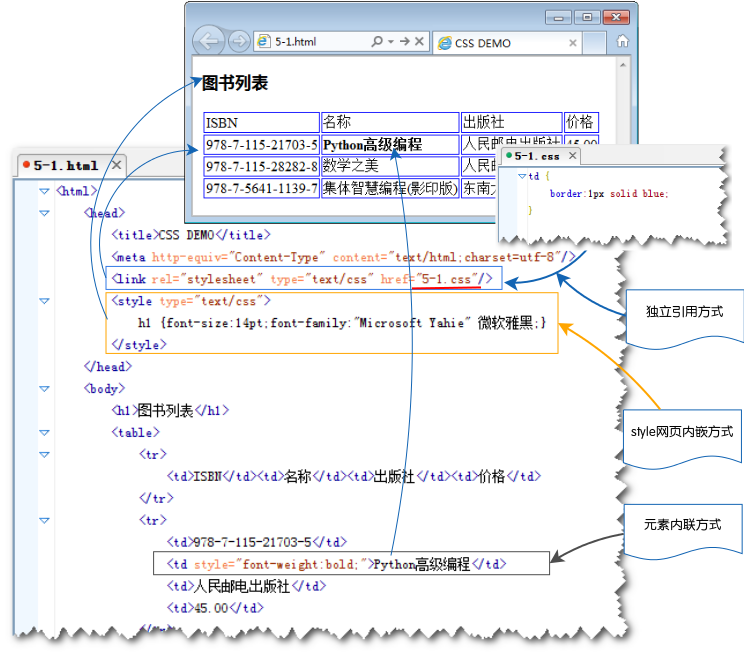
\includegraphics[width=0.75\textwidth]{figure/css-html-association.png}
\end{figure}
\end{frame}


\subsubsection{5.2.2 CSS与XML的关联方式}
\begin{frame}[fragile]{5.2.2 CSS与XML的关联方式}
\begin{easylist} \easyitem
& \em{通过<?xml-stylesheet?>处理指令实现关联}
& 非W3C规定,但得到主流浏览器的支持,成为事实标准
\end{easylist}
\end{frame}


\begin{frame}[fragile, allowframebreaks]{CSS与XML关联示例}
\begin{lstlisting}[tabsize=8, basicstyle=\small\tt, language=CSS,  caption=books.css]
book {display:block; margin:5px;}

title {   width:200px; 
           border: 1px solid gray;
           display:inline-block;
           padding:2px;
           padding-left:10px;
}

price { width:50px; 
           border: 1px solid gray;
           display:inline-block;
           padding:2px;
}

press { width:200px; 
           border: 1px solid gray; 
           display:inline-block;
           padding:2px;
}

authors, pages, description, cover {display: none;}
\end{lstlisting}

\begin{lstlisting}[tabsize=8, basicstyle=\small\tt, language=XML,  caption=books.xml]
<?xml version="1.0"?>
<?xml-stylesheet type="text/css" href="books.css"?>
<books>
    <book isbn="978-1449319793" id="b1">
        <title lang="EN">Python for Data Analysis</title>
        <price currency="dollar">25.40</price>
        <authors>
            <author>Wes McKinney</author>
        </authors>
        <press>OReilly Media</press>
        <pages>470</pages>
        <description>Python for Data Analysis...</description>
        <cover>book-python.jpg</cover>
    </book>
    <book isbn="978-7-115-28282-8" id="b2">
        <title lang="CHN">数学之美</title>
        <price>45.00</price>
        <authors>
            <author>吴军</author>
        </authors>
        <press>人民邮电出版社</press>
        <pages>304</pages>
        <description>读了“数学之美”,才发现大学时...</description>
        <cover>book-math.jpg</cover>
    </book>
</books>
\end{lstlisting}
\end{frame}


\subsection{5.3 CSS语法基础}
\begin{frame}[fragile]{5.3 CSS语法基础}
\begin{easylist} \easyitem
& CSS基本语法
& CSS选择器
& 继承与覆盖
\end{easylist}
\end{frame}

\subsubsection{5.3.1 CSS基本语法}
\begin{frame}[fragile, allowframebreaks]{5.3.1 CSS基本语法}
\begin{easylist} \easyitem
& 选择器 + 规则声明
& 形式:选择符 \{属性名: 属性值[; 属性名: 属性值]…\}
\begin{figure}
    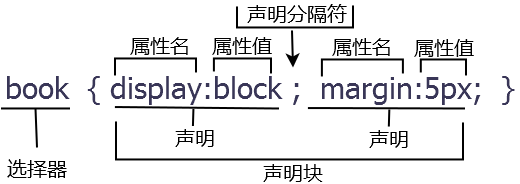
\includegraphics[width=0.75\textwidth]{figure/css-rule.png}
\end{figure}
&& 选择符(selector)
&&& 被施加样式的元素标记名(tag)、类([tag].class)或标识符([tag]\#id)等
&& 属性名称
&&& 表示颜色、字体等需要指定样式的名称
&& 属性值
&&& 表示属性具体的取值,如颜色取red,字体大小取12pt等
&& 英文冒号和分号作分隔
\end{easylist}
\end{frame}


\subsubsection{5.3.2 CSS选择器}
\begin{frame}[fragile]{5.3.2 CSS选择器}
\begin{easylist} \easyitem
& 元素选择器
& ID选择器
& 属性选择器
& 类选择器
& 通用选择器
& 分组选择器
& 后代选择器
\end{easylist}
\end{frame}


\begin{frame}[fragile]{元素选择器}
\begin{easylist} \easyitem
& 以元素名称作为选择器的表示方式,选择文档中的指定元素,是最常见的CSS选择方式
& 例子
\begin{lstlisting}[tabsize=8, basicstyle=\small\tt, language=CSS, numbers=none]
title {color: blue;}
\end{lstlisting}
\end{easylist}
\end{frame}


\begin{frame}[fragile]{ID选择器}
\begin{easylist} \easyitem
& 选择文档中具有特定id的元素
&& 在通过在id值前面附加字符“\#”作为选择器的表示方式
& 例子
\begin{lstlisting}[tabsize=8, basicstyle=\small\tt, language=CSS, numbers=none]
#b1 {color: red;}
\end{lstlisting}
\end{easylist}
\end{frame}


\begin{frame}[fragile]{属性选择器}
\begin{easylist} \easyitem
& 选择具有某个属性的元素集合
&& 将具有属性名称为lang的title元素的字体颜色设为橙色:
\begin{lstlisting}[tabsize=8, basicstyle=\small\tt, language=CSS, numbers=none]
title[lang] {color: orange;}
\end{lstlisting}
&& 将元素名称更改为星号可选择具有特定属性名称的任意元素即可
\begin{lstlisting}[tabsize=8, basicstyle=\small\tt, language=CSS, numbers=none]
*[isbn] {color:green;}
\end{lstlisting}
&& 选择具有特定属性名称和属性值的元素集合
\begin{lstlisting}[tabsize=8, basicstyle=\small\tt, language=CSS, numbers=none]
title[lang="CHN"] {color: red;}
\end{lstlisting}
\end{easylist}
\end{frame}


\begin{frame}[fragile]{类选择器}
\begin{easylist} \easyitem
& 选择具有特性class属性的元素集合,应用于HTML
& 例子
\begin{lstlisting}[tabsize=8, basicstyle=\small\tt, language=HTML, numbers=none]
<h1 class="important">这是重要标题</h1>
<p class="important">这是重要段落</p>
\end{lstlisting}
\begin{lstlisting}[tabsize=8, basicstyle=\small\tt, language=CSS, numbers=none]
.important{color: red;}
\end{lstlisting}
\end{easylist}
\end{frame}


\begin{frame}[fragile]{通用选择器}
\begin{easylist} \easyitem
& 星号“*”,匹配文档树中任何类型的元素名
& 例如:
\begin{lstlisting}[tabsize=8, basicstyle=\small\tt, language=CSS, numbers=none]
* {color: blue;}
\end{lstlisting}
& 非单独出现的通用选择器可以省略
\begin{lstlisting}[tabsize=8, basicstyle=\small\tt, language=CSS, numbers=none]
*[lang="CHN"] {color: red;} 等价于 [lang="CHN"] {color: red;}
*#b1 {color: red;} 等价于 #b1 {color: red;}
\end{lstlisting}
\end{easylist}
\end{frame}


\begin{frame}[fragile]{分组选择器}
\begin{easylist} \easyitem
& 一次选择多个元素
& 例子
\begin{lstlisting}[tabsize=8, basicstyle=\small\tt, language=CSS, numbers=none]
title, press {color: red;}
\end{lstlisting}
\end{easylist}
\end{frame}


\begin{frame}[fragile]{后代选择器}
\begin{easylist} \easyitem
& 把选中的元素限定在某些特定的文档结构中
& 例子
\begin{lstlisting}[tabsize=8, basicstyle=\small\tt, language=CSS, numbers=none]
#b1 title {color: blue;}
\end{lstlisting}
&& 将选中具有ID属性值为b1的元素内部的所有title子元素,并将其颜色设为蓝色
&& 后代选择器可选中任意符合选择器要求的后代元素
& 子元素选择器
&& 限定子元素
\begin{lstlisting}[tabsize=8, basicstyle=\small\tt, language=CSS, numbers=none]
book > title {color: blue;}
\end{lstlisting}
\end{easylist}
\end{frame}


\subsubsection{5.3.3 CSS的继承与覆盖}
\begin{frame}[fragile]{5.3.3 CSS的继承与覆盖}
\begin{easylist} \easyitem
& 属性继承
&& 子元素自动采用父元素中指定的样式作为本身的默认样式
& 属性覆盖
&& 一个元素最近指定的样式属性会覆盖之前指定的样式属性
\end{easylist}
\end{frame}


\begin{frame}[fragile]{支持继承的CSS属性}
\begin{easylist} \easyitem
& color
& font及相关属性
& letter-spacing
& line-height
& list-style及相关的属性
& text相关属性
& ...
\end{easylist}
\end{frame}


\begin{frame}[fragile]{不支持继承的CSS属性}
\begin{easylist} \easyitem
& background及相关属性
& border 及相关属性
& display
& float 和 clear
& margin及相关属性
& ...
\end{easylist}
\end{frame}


\begin{frame}[fragile]{属性覆盖原则-1}
\begin{easylist} \easyitem
& 当因继承而发生样式冲突时,最近祖先的样式将覆盖更远祖先的样式
\begin{lstlisting}[tabsize=8, basicstyle=\small\tt, language=CSS, numbers=none]
books {color:blue; }
book {color:red; }
\end{lstlisting}
\end{easylist}
\end{frame}


\begin{frame}[fragile]{属性覆盖原则-2}
\begin{easylist} \easyitem
& 当直接指定的样式与继承样式冲突时,将采用直接指定的样式
\begin{lstlisting}[tabsize=8, basicstyle=\small\tt, language=CSS, numbers=none]
books {color:blue; }
book {color:red; }
title {color:orange; }
\end{lstlisting}
\end{easylist}
\end{frame}


\begin{frame}[fragile]{属性覆盖原则-3}
\begin{easylist} \easyitem
& 当直接指定的样式发生冲突时,采用权重高者的样式
\begin{lstlisting}[tabsize=8, basicstyle=\small\tt, language=CSS, numbers=none]
book {color:blue; }
#b1 {color:red; }
\end{lstlisting}
&& ID选择器的权重高于元素选择器,因此,ID为b1的图书内容将以红色字体显示
\end{easylist}
\end{frame}


\begin{frame}[fragile]{属性覆盖原则-4}
\begin{easylist} \easyitem
& 当样式权重相同时,采用最后指定的样式
\begin{lstlisting}[tabsize=8, basicstyle=\small\tt, language=CSS, numbers=none]
book title[lang] {color: blue;}
book[isbn] title {color: red;}
\end{lstlisting}
\end{easylist}
\end{frame}


\begin{frame}[fragile]{属性覆盖原则-5}
\begin{easylist} \easyitem
& !important的样式属性不被覆盖
\begin{lstlisting}[tabsize=8, basicstyle=\small\tt, language=CSS, numbers=none]
book {color:blue !important; }
#b1 {color:red; }
\end{lstlisting}
&& 虽然ID选择器的权重高于元素选择器,但由于book元素选择器中的样式指定了!important,从而使ID为b1的图书元素强制显示为蓝色
\end{easylist}
\end{frame}



\subsection{5.4 CSS重要属性}
\begin{frame}[fragile]{5.4 CSS重要属性}
\begin{easylist} \easyitem
& 颜色属性
& 字体属性
& 文本属性
& 盒状模型相关属性
& 可视格式化模型相关属性
\end{easylist}
\end{frame}


\subsubsection{5.4.1 颜色属性}
\begin{frame}[fragile]{5.4.1 颜色属性}
\begin{easylist} \easyitem
& 名称表示方式
&& black, white, blue, yellow, red, ...
& RGB表示方式
&& \#rrggbb
&&& 两位十六进制数字(00~FF)分别表示红绿蓝三种颜色的分量取值, 如:\#FF0000
&& \#rgb 
&&& 等价于 \#rrggbb,如:\#F00
&& RGB(r, g, b)
&&& 以十进制指定红绿蓝颜色分量值,如: RGB(255,0,0)
&& RGB(r\%, g\%, b\%)
&&& 用百分比表示红绿蓝分量比重,如: RGB(100\%, 0\%, 0\%)
\end{easylist}
\end{frame}


\begin{frame}[fragile]{颜色名称和RGB值}
\begin{figure}
    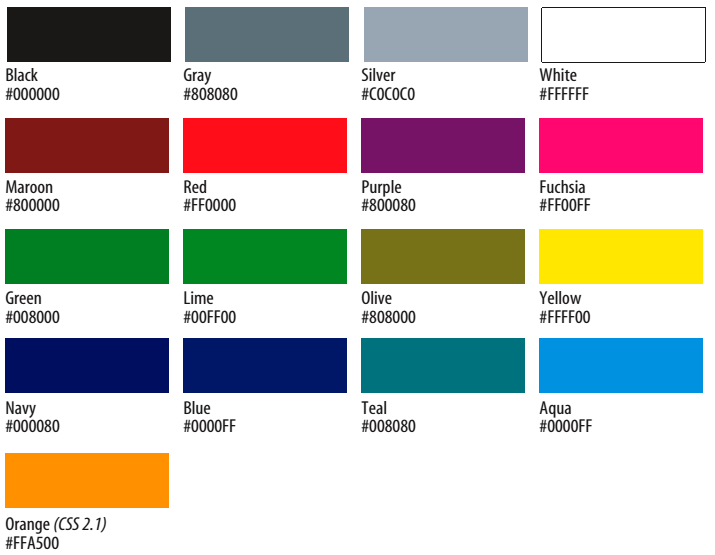
\includegraphics[width=0.75\textwidth]{figure/css-colors.png}
\end{figure}
\end{frame}


\begin{frame}[fragile]{颜色示例}
\begin{lstlisting}[tabsize=8, basicstyle=\small\tt, language=CSS]
book {display:block; margin:5px; }
title { width:200px; border: 1px solid gray;
        display:inline-block;padding:2px;padding-left:10px;}
price { width:50px; border: 1px solid gray;
        display:inline-block;padding:2px;}
press { width:200px; border: 1px solid gray;
        display:inline-block;padding:2px;}
authors, pages, description, cover {display: none;}

title {color: blue;}
price {color: #FFA500; }
press {color:RGB(255, 0, 0);}
\end{lstlisting}
\end{frame}


\begin{frame}[fragile]{浏览器中的呈现效果}
\begin{figure}
    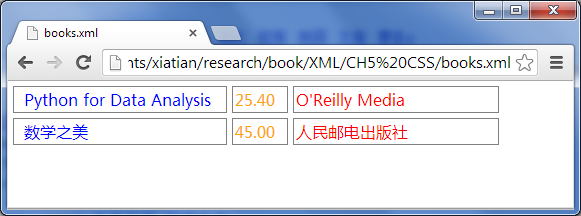
\includegraphics[width=0.75\textwidth]{figure/css-color-demo.png}
\end{figure}
\end{frame}


\subsubsection{5.4.2 字体属性}
\begin{frame}[fragile]{5.4.2 字体属性}
\begin{easylist} \easyitem
& 字体族font-family
& 字体风格font-style
&& normal | italic | oblique | inherit
& 字体变体font-variant
&& normal | small-caps | inherit
& 字体粗细font-weight
&& normal | bold | bolder | lighter | 100 | 200 | 300 | 400 | 500 | 600 | 700 | 800 | 900 | inherit
& 字体大小font-size
\end{easylist}
\end{frame}


\begin{frame}[fragile]{font-family}
\begin{easylist} \easyitem
& 定义文本所使用的字体族
&& 字体族由一系列相关字体组成,如微软雅黑字体作为一个字体族会包括大小、粗体、斜体等不同显示效果的字体
& family-name(字体族名称)
&& 通常所说的“字体”,如“Arial”、“Times New Roman”、“宋体”、“微软雅黑”等
& generic family(族类名称)
&& 一组具有统一外观的字体族,它包含的范围比family-name更大,可看作是一组具有某些共同特点的family-name的集合
\end{easylist}
\end{frame}


\begin{frame}[fragile]{Generic Family: Serif、Sans-serif and Monospace}
\begin{figure}
    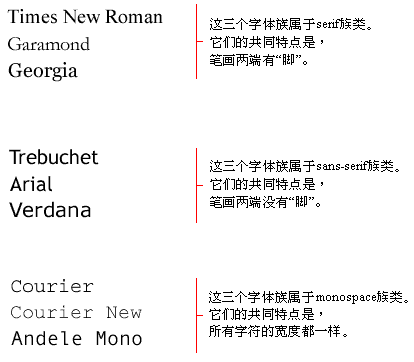
\includegraphics[width=0.75\textwidth]{figure/css-generic-family.png}
\end{figure}
\end{frame}


\begin{frame}[fragile, allowframebreaks]{font-size}
\begin{easylist} \easyitem
& 绝对大小<absolute-size> 
&& xx-small | x-small | small | medium | large | x-large | xx-large
& 相对大小<relative-size>
&&  larger | smaller 
& 指定长度<length>
&& 相对长度单位:
&&& em: the ‘font-size’ of the relevant font
&&& ex: the ‘x-height’ of the relevant font
&&& \em{px: pixels, 像素,相对于显示设备的最小显示单位}
&& 绝对长度单位:
&&& in: inches,英寸,一英寸约等于2.54厘米
&&& cm: centimeters,厘米
&&& mm: millimeters,毫米
&&& \em{pt: pofints,等于1/72英寸}
&&& pc: picas,等于12 points
& 百分比<percentage>
&& 相对于继承的字体大小的百分比
\end{easylist}
\end{frame}


\begin{frame}[fragile, allowframebreaks]{例子}
\begin{lstlisting}[tabsize=8, basicstyle=\small\tt, language=CSS,  caption=books-font.css]
book {display:block; margin:5px; }
title { width:200px; border: 1px solid grey;
    display:inline-block;padding:2px;padding-left:10px;
}
price { width:50px; border: 1px solid grey;
    display:inline-block;padding:2px;
}
press { width:200px; border: 1px solid grey; 
    display:inline-block;padding:2px;
}
authors, pages, description, cover {display: none;}

book {font-family: “Times New Roman”, “微软雅黑”, Serif;}
title {font-weight:bold;}
press {font-variant:small-caps;}
book#b2 title {font-size: larger;}
book#b2 price {font-size: 10pt;}
\end{lstlisting}
\begin{figure}
    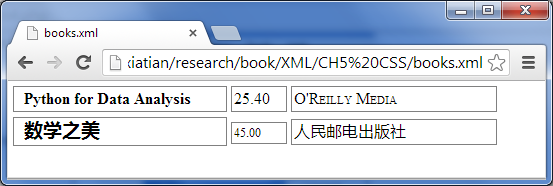
\includegraphics[width=0.75\textwidth]{figure/css-font-demo.png}
\end{figure}
\end{frame}



\begin{frame}[fragile, allowframebreaks]{font}
\begin{easylist} \easyitem
& 字体样式的简写方式
&& 顺序: font-style | font-variant | font-weight | font-size | font-family
& 以下两段代码等价:
\begin{lstlisting}[tabsize=8, basicstyle=\small\tt, language=CSS]
title {
    font-style: italic;
    font-weight: bold;
    font-size: 16px;
    font-family: arial, sans-serif;
}
\end{lstlisting}
\begin{lstlisting}[tabsize=8, basicstyle=\small\tt, language=CSS]
title { 
    font: italic bold 16px arial,sans-serif;
}
\end{lstlisting}
\end{easylist}
\end{frame}



\subsubsection{5.4.3 文本属性}
\begin{frame}[fragile, allowframebreaks]{5.4.3 文本属性}
\begin{easylist} \easyitem
& text-indent(文本缩进)
&& 设置文本块中首行文本的缩进或悬挂,缺省值为0(不缩进)
\begin{lstlisting}[tabsize=8, basicstyle=\small\tt, language=CSS, numbers=none]
title { text-indent: 3em; } 
\end{lstlisting}
&&& 例如将title元素内容缩进3个字

& text-align(文本对齐)
&& 设置文本段的对齐特性
&& 取值:
&&& left(左对齐)
&&& right(右对齐)
&&& center(居中)
&&& justify(两端撑满)
&&& inherit(继承)

& text-decoration(文本修饰)
&& 取值可以为:
&&& none(无修饰,为缺省值)
&&& underline(下划线)
&&& overline(上划线)
&&& line-through(删除线)
&&& blink(闪烁)
&&& inherit(继承)

& letter-spacing(字母间隔)和 word-spacing(词间隔)
&& 取值均可以为
&&& normal(缺省值)
&&& 指定长度
&&& inherit(继承)

& text-transform(文本转换)
&& 用于进行大小写转换
&&& capitalize——每个单词的首字母大写,其他字母不变
&&& uppercase——所有字母全大写
&&& lowercase——所有字母全小写
&&& none——不转换,使用默认值,为缺省值
&&& inherit——继承

& white-space(空白)
&& 设置对文本中对空白符的处理方法
&&& normal——收缩白空序列,自动换行,为缺省值
&&& pre——防止(prevent)白空序列收缩,保留白空符不变
&&& nowrap——收缩白空序列,但抑制换行
&&& pre-wrap——不收缩白空序列,在源文本的回车和换行处换行,并在需要的地方自动换行
&&& pre-line——收缩白空序列,在源文本的回车和换行处换行,并在需要的地方自动换行
\end{easylist}
\end{frame}


\begin{frame}[fragile, allowframebreaks]{例子}
\begin{lstlisting}[tabsize=8, basicstyle=\small\tt, language=CSS,  caption=books-font.css]
book {display:block; margin:5px; }
title { width:250px; border: 1px solid gray;
            display:inline-block;padding:2px;padding-left:10px;}
price { width:50px; border: 1px solid gray;
            display:inline-block;padding:2px;}
press { width:250px; border: 1px solid gray; 
            display:inline-block;padding:2px;}
authors, pages, description, cover {display: none;}

title {
            text-indent:1em; 
            text-decoration:underline;
            letter-spacing:0.1em;
}
press {
            text-align:center; 
            word-spacing:1cm;
            text-transform:uppercase;
}
\end{lstlisting}
\begin{figure}
    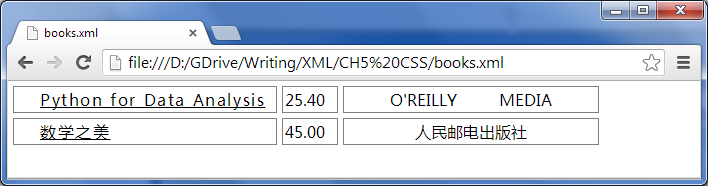
\includegraphics[width=0.75\textwidth]{figure/css-text-demo.png}
\end{figure}
\end{frame}



\subsubsection{5.4.4 盒状模型相关属性}
\begin{frame}[fragile]{5.4.4 盒状模型相关属性}
\begin{figure}
    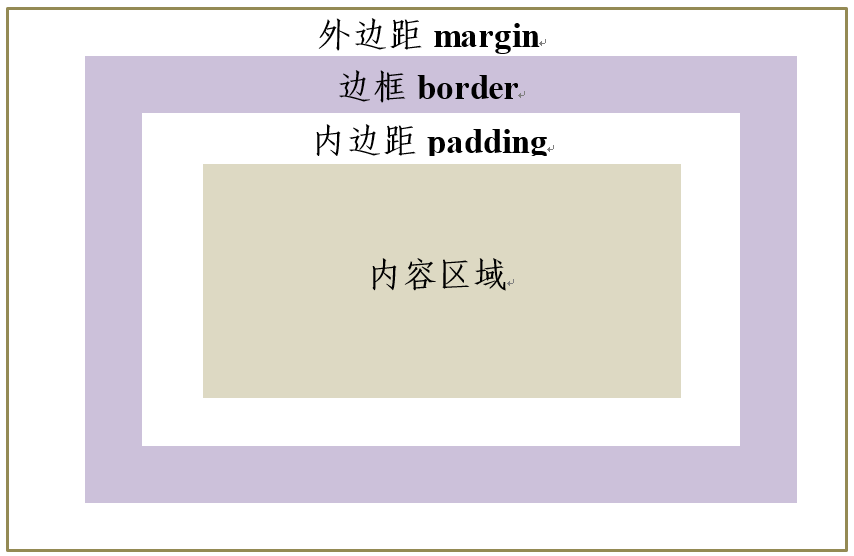
\includegraphics[width=0.60\textwidth]{figure/css-box-model.png}
\end{figure}
\begin{easylist} \easyitem
& 盒状模型
&& margin
&& padding
&& border
\end{easylist}
\end{frame}


\begin{frame}[fragile]{padding}
\begin{easylist} \easyitem
& 简写方式:直接指定一个数值
\begin{lstlisting}[tabsize=8, basicstyle=\small\tt, language=CSS, numbers=none]
title { padding:2px; } 
\end{lstlisting}
& 按照上、右、下、左的顺时针方向顺序分别设置各边的内边距
\begin{lstlisting}[tabsize=8, basicstyle=\small\tt, language=CSS, numbers=none]
title { padding: 2px 5% 5px 2%;}
\end{lstlisting}
& 分别设置
&& padding-top
&& padding-right
&& padding-bottom
&& padding-left
\end{easylist}
\end{frame}


\begin{frame}[fragile]{margin}
\begin{easylist} \easyitem
& 简写方式:直接指定一个数值
\begin{lstlisting}[tabsize=8, basicstyle=\small\tt, language=CSS, numbers=none]
book { margin: 10px;}
\end{lstlisting}
& 按照上、右、下、左的顺时针方向顺序分别设置各边的外边距
\begin{lstlisting}[tabsize=8, basicstyle=\small\tt, language=CSS, numbers=none]
book { margin: 5px 10px 5px 5%;}
\end{lstlisting}
& 分别设置
&& margin-top
&& margin-right
&& margin-bottom
&& margin-left
\end{easylist}
\end{frame}


\begin{frame}[fragile]{border}
\begin{easylist} \easyitem
& border-width
\begin{lstlisting}[tabsize=8, basicstyle=\small\tt, language=CSS, numbers=none]
title {border-width: medium;}
price {border-width: 2px;}
\end{lstlisting}

& border-color
\begin{lstlisting}[tabsize=8, basicstyle=\small\tt, language=CSS, numbers=none]
title {border-color: red;}
\end{lstlisting}

& border-style
\begin{lstlisting}[tabsize=8, basicstyle=\small\tt, language=CSS, numbers=none]
book {border-style: solid;}
\end{lstlisting}
\end{easylist}
\end{frame}



\begin{frame}[fragile]{border简写方式}
\begin{easylist} \easyitem
& 以下两段代码等价
\begin{lstlisting}[tabsize=8, basicstyle=\small\tt, language=CSS]
title {
    border-width: 2px;
    border-style: solid;
    border-color: red;
}
\end{lstlisting}
\begin{lstlisting}[tabsize=8, basicstyle=\small\tt, language=CSS, numbers=none]
title { border: 2px solid red;}
\end{lstlisting}
\end{easylist}
\end{frame}


\begin{frame}[fragile]{练习}
\begin{easylist} \easyitem
& 通过CSS控制“books.xml”显示效果,在“books.css”的基础上,满足以下要求:
&& title、price和press元素仅显示2个像素、灰色的实线下边框
&& 每行图书下面的外边距为15个像素
&& price元素的左侧内边距为20个像素
\end{easylist}
\end{frame}


\subsubsection{5.4.5 可视格式化模型相关属性}
\begin{frame}[fragile]{5.4.5 可视格式化模型相关属性}
\begin{easylist} \easyitem
& 可视格式化模型VFM: Visual Formatting Model
&& 每个元素会依据盒状模型生成0个或多个盒子
&& 盒子的布局由盒的尺寸和类型、定位方案、文档树中元素间的关系、以及外部信息所控制
&& 包括显示、高度、宽度、定位、文本方向等属性
\end{easylist}
\end{frame}


\begin{frame}[fragile]{display显示属性}
\begin{easylist} \easyitem
& display显示属性
&& 用于设置和改变元素所对应的盒子的显示类型
&& 元素既可以显示为独立的一块内容,即块元素
&& 也可以显示在一行中,即行内元素
\end{easylist}
\end{frame}


\begin{frame}[fragile]{display属性常见取值及作用}
\begin{table}[!hbp] 
\begin{tabular}{|l|l|}
\Xhline{1.3pt}
display属性取值 & 作用\\ \Xhline{1.3pt}
block & 使元素产生一个块状盒子,并换行\\ \hline
inline-block & 产生一个行内(inline)块状盒子,不强制换行\\ \hline
inline & 产生一个或多个行内盒子,缺省值\\ \hline
list-item & 产生一个主块和一个表项行内盒\\ \hline
none & 不产生盒子,即无布局效果\\ \hline
\end{tabular}
\end{table}
\end{frame}


\begin{frame}[fragile]{宽度和高度属性}
\begin{easylist} \easyitem
& 宽度属性width
&& 指定由块级元素和替换元素所生成的盒子的内容宽度
&& 取值可以为长度或百分比
& 高度属性height
&& 用于对元素盒子的高度进行限定,
&& 取值同样为长度值或百分比
& 例子
\begin{lstlisting}[tabsize=8, basicstyle=\small\tt, language=CSS, numbers=none]
title{height:30px; width:500px;}
\end{lstlisting}
&& 指定title元素的高度和宽度分别为30个像素和500个像素大小
\end{easylist}
\end{frame}



\begin{frame}
\begin{center}
    \Huge END
\end{center}
\begin{figure}
    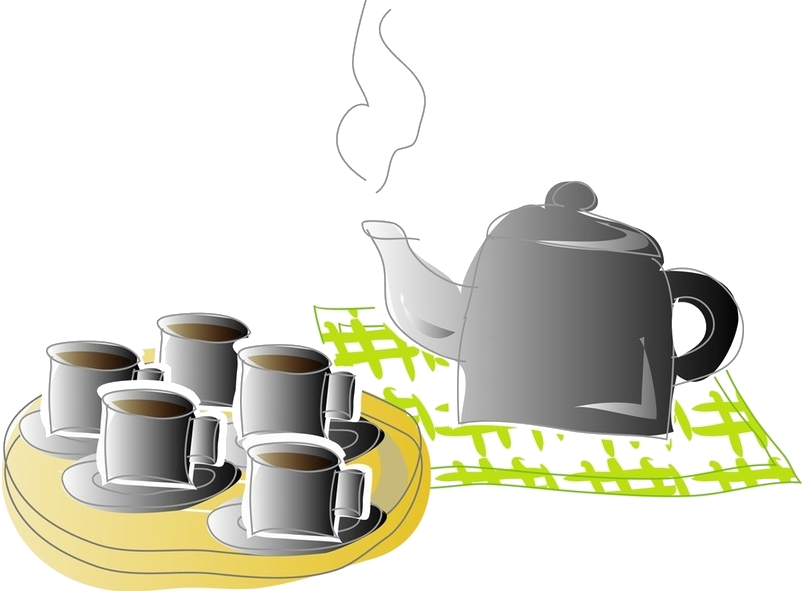
\includegraphics[width=0.75\textwidth]{figure/relax.png}
\end{figure}
\end{frame}

%\section{ XML路径语言XPath}

\begin{frame}[fragile]{CH6 XML路径语言XPath}
\begin{figure}
    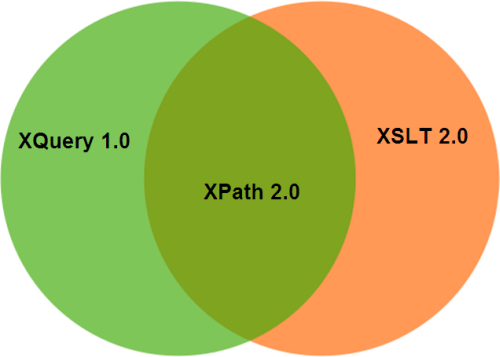
\includegraphics[width=0.5\textwidth]{figure/xpath.png}
\end{figure}
\end{frame}

\begin{frame}[fragile, allowframebreaks]{本章学习目标}
\begin{easylist} \easyitem
& 了解XPath的工作原理
& 掌握XPath的定位路径表达式
& 熟悉XPath的常用函数和数据类型
& 掌握XPath2.0的部分新特性
\end{easylist}
\end{frame}

\begin{frame}[fragile, allowframebreaks]{目录}
\begin{easylist} \easyitem
& XPath概述
&& XPath及其作用
&& XPath工作原理
&& XPath的表达式与操作符
&& 如何测试XPath

& XPath结点与结点集
&& 结点的基本属性
&& 结点类型
&& 结点集

& XPath定位路径表达式
&& XPath定位步骤
&& XPath轴
&& 结点测试
&& 谓词
&& 定位路径缩写

& XPath的基本表达式
&& 布尔表达式
&& 等式表达式
&& 关系表达式
&& 数值表达式

& XPath数据类型
&& 字符串类型
&& 数值类型
&& 布尔类型
&& 结点集类型

& XPath 1.0常用函数
& XPath 2.0
\end{easylist}
\end{frame}


\subsection{6.1 概述}

\begin{frame}[fragile]{6.1 概述}
\begin{easylist} \easyitem
& 考虑以下问题
&& 从存储图书信息的XML文档中选择指定ISBN号码的图书标题信息
&& 从XML文档中排除掉某些信息再进行处理
&&& 例如:当显示员工信息时,把工资信息隐藏掉不予显示
&& \em{如何从XML文档中选择部分结点或结点集合,实现对XML文档中的元素、属性等信息的定位和查找,准确快速的找到XML文档结构树中的任意一个或一组结点}
\end{easylist}
\end{frame}


\subsubsection{6.1.1 XPath及其作用}
\begin{frame}[fragile]{6.1.1 XPath及其作用}
\begin{easylist} \easyitem
& XPath
&& XML Path Language
&& 把整个XML文档看成是一棵由结点组成的层次树,通过结点路径进行定位
&& XPath 1.0
&&& 1999年11月16发布,作为XSLT和XPointer的配套标准,用于XML文档的寻址
&& XPath 2.0
&&& XPath 1.0的超集,增加了丰富的数据类型
\end{easylist}
\end{frame}


\begin{frame}[fragile]{6.1.1 XPath及其作用}
\begin{easylist} \easyitem
& XPath的作用
&& XPath为XML文档提供一种快捷方便并易于使用的寻址功能,实现对XML文档树中指定结点或结点集合的选择定位。
&& XPath为XML其他相关技术提供核心支持,包括XSLT、XQuery、XPointer、XForm等。
&& XPath为人们处理XML文档提供了一种标准通用规范,XPath的公共API接口独立于特定语言,使得对XML文档的操纵处理更为方便
\end{easylist}
\end{frame}


\subsubsection{6.1.2 XPath的工作原理}
\begin{frame}[fragile]{6.1.2 XPath的工作原理}
\begin{easylist} \easyitem
& 从内容构成来看,XML文档与普通的文本文件相同,因此又称为序列化XML文档(Serialized XML Document)
& XML更注重逻辑结构特征,目前三个从不同角度描述XML文档的逻辑模型
&& XPath
&& DOM
&& XML信息集合(XML Information Set)
\end{easylist}
\end{frame}


\begin{frame}[fragile]{XPath数据模型}
\begin{easylist} \easyitem
& XPath把XML文档看成是一个或一组文档树结点,文档的大部分内容都表示为结点
& XML文档的特殊部分没有对应的XPath表示方式
&& 例如:最开始的XML声明语句
\end{easylist}
\end{frame}


\begin{frame}[fragile]{文档对象模型DOM}
\begin{easylist} \easyitem
& 同样把整个XML文档表示成一棵由结点组成的层次树
& DOM和XPath在表示结点的方式上有所不同
&& DOM中的结点包含有丰富的信息,更多的应用于XML编程处理方面
&& 例如DOM结点对象有类型、属性、方法等概念
\end{easylist}
\end{frame}


\begin{frame}[fragile]{XML信息集合}
\begin{easylist} \easyitem
& 也叫XML信息集
& XML信息集是XML文档的纯信息表示,适用于从XML角度而非文本角度比较两个文件的异同
&& 信息集不区分空元素的两种形式
&& 属性所使用的引号类型也不重要,克服了严格的文本字符比较的缺点
\end{easylist}
\end{frame}


\begin{frame}[fragile, allowframebreaks]{文本不同但信息集合角度相同的两个XML文档}
\begin{lstlisting}[tabsize=8, basicstyle=\small\tt, language=XML, caption=''6-1.xml'']
<?xml version="1.0" encoding="UTF-8"?>
<order id="TEST-01">
    <?backup dbname="order"?>
    <product name="打印纸" price="30" quantity="5"/>
    <product name="圆珠笔" price="2" quantity="10"/>
    <product name="铅笔" price="1.5" quantity="10"/>
    <product name="白板" price="80" quantity="2"/>
</order>
\end{lstlisting}

\newpage
\begin{lstlisting}[tabsize=8, basicstyle=\small\tt, language=XML, caption=''6-2.xml'']
<order id='TEST-01' >
    <?backup dbname="order"?>
    <product name='打印纸' price='30' quantity='5'/>
    <product name='圆珠笔' price='2' quantity='10'/>
    <product name='铅笔' price='1.5' quantity='10'/>
    <product name='白板' price='80' quantity='2'/>
</order>
\end{lstlisting}
\end{frame}


\begin{frame}[fragile]{XPath}
\begin{figure}
    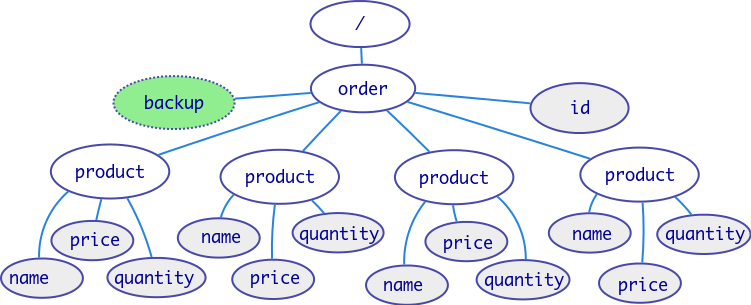
\includegraphics[width=0.75\textwidth]{figure/xpath-tree.png}
\end{figure}
\begin{easylist} \easyitem
& 利用结点之间的层次关系实现定位
& 例子:
\begin{lstlisting}[tabsize=8, basicstyle=\small\tt, language=XML, numbers=none]
/order/product[2]/@name
\end{lstlisting}
\end{easylist}
\end{frame}


\subsubsection{6.1.3 XPath的表达式与操作符}
\begin{frame}[fragile]{6.1.3 XPath的表达式与操作符}
\begin{table}[!hbp] 
\begin{tabular}{l|l}
\Xhline{1.3pt}
表达式类型 &	操作符 \\ \Xhline{1.3pt}
定位路径表达式& /,  //,  |  \\ \hline
布尔表达式 & or,   and  \\ \hline
等式表达式 & =,   !=  \\ \hline
关系表达式 &	<=,  <,  >=,  >  \\ \hline
数值表达式 & 	+,  -,  div,  mod,  *,  -(unary)  \\ \hline
\end{tabular}
\end{table}
\end{frame}


\subsubsection{6.1.4 如何测试XPath}
\begin{frame}[fragile]{6.1.4 如何测试XPath}
\begin{figure}
    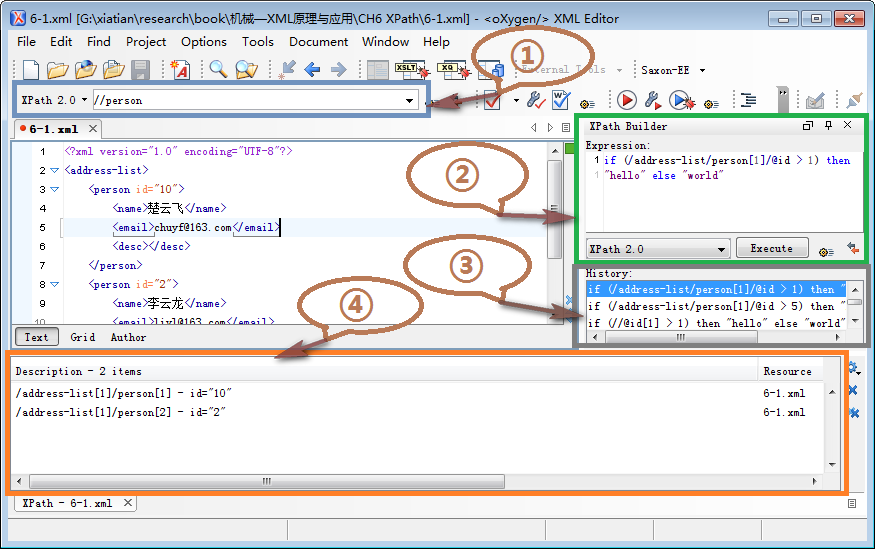
\includegraphics[width=0.85\textwidth]{figure/xpath-test-oxygen.png}
\end{figure}
\end{frame}



\subsection{6.2 XPath结点与结点集}
\begin{frame}[fragile]{6.2 XPath结点与结点集}
\begin{easylist} \easyitem
& 结点可看成是XPath定位步中用来实现定位功能的离散的、逻辑性的东西
&& XML文档中的任意一个元素、属性、处理指令、注释等,都可以是一个结点
& 结点集:结点组成的集合
\end{easylist}
\end{frame}


\subsubsection{6.2.1 结点的基本属性}
\begin{frame}[fragile]{6.2.1 结点的基本属性}
\begin{easylist} \easyitem
& 结点名称
& 结点顺序
& 结点之间的家族关系
\end{easylist}
\end{frame}


\begin{frame}[fragile]{结点名称}
\begin{easylist} \easyitem
& 大部分结点都用名称(根结点没有),三种名称:
&& 限定名称QName(Qualified name)
&&& XML文档实例中该结点的唯一标识符,包括结点的命名空间前缀部分
&&& <product>元素的QName为product
&&& <common:product>的QName为common:product

&& 本地名称(Local-name)
&&& QName去除命名空间前缀后剩余的内容
&&& 如果没有指定命名空间,其规范名称和本地名称完全相同
&&& <common:product>的本地名称为product

&& 扩展名称(Expended-name)
&&& 扩展名称由与命名空间关联的URI与本地名称共同构成
&&& 扩展名称不关心命名空间前缀的具体名称
\end{easylist}
\end{frame}


\begin{frame}[fragile]{结点顺序}
\begin{easylist} \easyitem
& 结点位置是由该结点前面的结点和后面的结点所决定的
& 通常按照先后顺序进行访问
& 借助于XPath坐标轴,也可以实现对XML文档结点的逆序访问或指定顺序访问
\end{easylist}
\end{frame}


\begin{frame}[fragile]{结点之间的家族关系}
\begin{easylist} \easyitem
& 结点之间通过XPath坐标轴维持关系
& 常见关系包括:
&& 相邻关系
&& 祖先关系
&& 子孙关系
&& ...
\end{easylist}
\end{frame}


\subsubsection{6.2.2 结点类型}
\begin{frame}[fragile]{6.2.1 结点的基本属性}
\begin{easylist} \easyitem
& 根节点
& 元素节点
& 属性节点
& 命名空间节点
& 处理指令节点
& 注释节点
& 正文节点
\end{easylist}
\end{frame}


\subsubsection{6.2.3 结点集}
\begin{frame}[fragile]{6.2.3 结点集}
\begin{easylist} \easyitem
& 由结点构成的集合
& 例如“6-1.xml”中,位置路径/order/product则返回一个包含了4个product元素的结点集
\end{easylist}
\end{frame}



\subsection{6.3 XPath定位路径表达式}
\begin{frame}[fragile]{6.3 XPath定位路径表达式}
\begin{easylist} \easyitem
& 由一个或多个定位步骤组成,每个定位步骤之间用斜线“/”分隔
& 如表达式以“/”开始,则称为绝对路径,否则称为相对路径
& 使用“/”符号作为定位步骤之间的分隔符
\end{easylist}
\end{frame}


\subsubsection{6.3.1 XPath定位步骤}
\begin{frame}[fragile]{6.3.1 XPath定位步骤}
\begin{easylist} \easyitem
& 定位步骤的组成
&& 轴:用来导航XPath数据模型的结点树的工具
&& 测试结点:用来确定选取轴中哪类结点
&& 谓词:可选步骤,用来过滤轴和定位方法所选取的结点集
\end{easylist}
\begin{figure}
    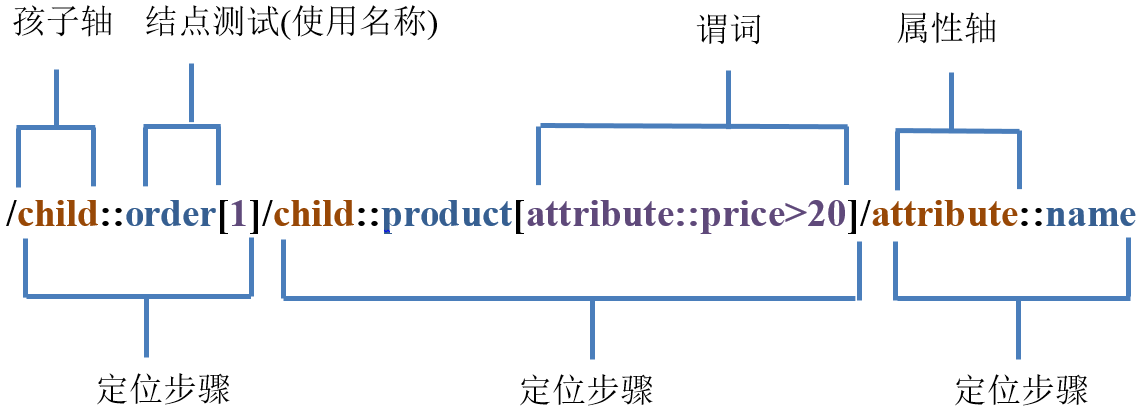
\includegraphics[width=0.75\textwidth]{figure/xpath-step.png}
\end{figure}
\end{frame}


\subsubsection{6.3.2 XPath轴}
\begin{frame}[fragile]{6.3.2 XPath轴: 在结点的哪一个方向上进行导航定位}
\begin{table}[!hbp] 
\begin{tabular}{l|l|l}
\Xhline{1.3pt}
轴 & 名称 & 方向  \\ \Xhline{1.3pt}
child & 子轴 & 前向 \\ \hline
parent & 双亲轴 & 不可用 \\ \hline
attribute & 属性轴 & 不可用 \\ \hline
ancestor & 祖先轴 & 反向 \\ \hline
ancestor-or-self & 祖先自身轴 & 反向 \\ \hline
descendant & 子孙轴 & 前向 \\ \hline
descendant-or-self & 子孙自身轴 & 前向 \\ \hline
following & 后继轴 & 前向 \\ \hline
following-sibling & 后继兄弟轴 & 前向 \\ \hline
preceding & 前驱轴 & 反向 \\ \hline
preceding-sibling & 前驱兄弟轴 & 	反向 \\ \hline
namespace & 命名空间轴 & 不可用 \\ \hline
self & 自身轴 & 不可用 \\ \hline
\end{tabular}
\end{table}
\end{frame}



\begin{frame}[fragile, allowframebreaks]{XPath轴示例}
\begin{easylist} \easyitem
& 示例文档
\begin{lstlisting}[tabsize=8, basicstyle=\small\tt, language=XML]
<?xml version="1.0" encoding="UTF-8"?> 
<abc:order id="TEST-01" xmlns:abc="http://www.abc.com" 
                    xmlns:abc2="http://www.abc2.com">
    <?backup dbname="order"?>
    <product name="打印纸" price="30" quantity="5"/>
    <product name="圆珠笔" price="2" quantity="10"/>
    <product name="铅笔" price="1.5" quantity="10"/>
    <product name="白板" price="80" quantity="2"/>
</abc:order>
\end{lstlisting}

\newpage
& 测试表达式:
\begin{lstlisting}[tabsize=8, basicstyle=\small\tt, language=XML, numbers=none]
/abc:order/namespace::abc
\end{lstlisting}

& 结果:
\begin{lstlisting}[tabsize=8, basicstyle=\small\tt, language=XML, numbers=none]
abc - http://www.abc.com
\end{lstlisting}

& 测试表达式:
\begin{lstlisting}[tabsize=8, basicstyle=\small\tt, language=XML, numbers=none]
/abc:order/namespace::node()
\end{lstlisting}

& 结果:
\begin{lstlisting}[tabsize=8, basicstyle=\small\tt, language=XML, numbers=none]
xml - http://www.w3.org/XML/1998/namespace
abc - http://www.abc.com
abc2 - http://www.abc2.com
\end{lstlisting}
\end{easylist}
\end{frame}


\subsubsection{6.3.3 结点测试}
\begin{frame}[fragile]{6.3.3 结点测试}
\begin{easylist} \easyitem
& 用于确定轴中的结点,只有给定结点的结点测试结果为true,该结点才会保留在结点集中
& 使用名称进行测试,例如:
&& child::brandA:product
&& 选中QName为brandA:product的所有孩子元素结点
& 使用类型进行测试,例如:
&& child::text( )	
&& 确定文本子结点
& 参考教材内容
\end{easylist}
\end{frame}


\subsubsection{6.3.4 谓词}
\begin{frame}[fragile]{6.3.4 谓词}
\begin{easylist} \easyitem
& 谓词是指针对条件表达式进行求值返回真或假的过程
& 谓词置于定位步骤末端的方括号中,用于筛选一个结点集以生成新的结点集
& 针对结点集中每一个被筛选的结点,谓词表达式将此结点作为上下文结点进行求值,如为true,则保留在结点集中,否则,从结点集中删除
& 例子:
&& descendant::product[attribute::price > 20]	
&& 选择product的子孙元素,且product元素拥有大于20的price属性
\end{easylist}
\end{frame}


\subsubsection{6.3.5 定位路径缩写}
\begin{frame}[fragile]{6.3.5 定位路径缩写}
\begin{table}[!hbp] 
\begin{tabular}{l|l}
\Xhline{1.3pt}
示例 & 对应缩写示例 \\ \Xhline{1.3pt}
child::product & product \\ \hline
child::product/attribute::name & product/@name \\ \hline
self::node()/product & ./product \\ \hline
parent::node()/@name & ../@name \\ \hline
/descendant-or-self::node()/product & //product \\ \hline
child::product[position( ) == 3] & product[3] \\ \hline
\end{tabular}
\end{table}
\end{frame}



\subsection{6.4 XPath基本表达式}
\begin{frame}[fragile]{6.4 XPath基本表达式}
\begin{easylist} \easyitem
& 布尔表达式:and or
&& person[name and age]
&& person[(age>30) or (age<50)]
& 等式表达式: =, !=
&& age = 30
&& age != 30
& 关系表达式:<, <=, >, >=
&& age <= 30
& 数值表达式:+, -, div, mod, * -(unary)
&& person[(age mod 2) =0]
&& 选择具有偶数数值age子元素的person子元素
\end{easylist}
\end{frame}



\subsection{6.5 XPath数据类型}
\begin{frame}[fragile]{6.5 XPath数据类型}
\begin{easylist} \easyitem
& 字符串类型
&& person[name='李云龙']
& 数值类型
&& <pages>102</pages>
&& pages + 10
& 布尔类型
&& order[@id="1"]
& 结点集类型、
&& //book
\end{easylist}
\end{frame}


\subsection{6.6 XPath 1.0常用函数}
\begin{frame}[fragile]{6.6 XPath 1.0常用函数}
\begin{easylist} \easyitem
& 结点集相关函数
& 布尔函数
& 数值函数
& 字符串函数
\end{easylist}
\end{frame}


\subsection{6.6.1 结点集函数}
\begin{frame}[fragile]{6.6.1 结点集函数}
\begin{easylist} \easyitem
& last()
&& 返回上下文的大小,即给定上下文中的节点数。
& position()
&& 返回上下文结点的位置。比如,可以用表达式 position()=last() 测试处理的是否是集合中最后一个节点。
& count()
&& 参数为结点集,返回这个结点集中包含的结点个数。
& id()
&& 参数为字符串,返回一个结点集,结点集中的每一个结点的ID属性值等于这个参数字符串。
XPath中的另外三个与结点集相关的函数为:
\end{easylist}
\end{frame}


\subsection{6.6.2 布尔函数}
\begin{frame}[fragile]{6.6.2 布尔函数}
\begin{easylist} \easyitem
& boolean()
&& 以对象为参数,返回一个布尔值。当参数是一个非0数值时,返回true,为数值0时,返回false;当参数为字符串时,返回true;如参数为结点集并且非空,返回true,否则为false。
& not()
\end{easylist}
\end{frame}


\subsection{6.6.3 数值函数}
\begin{frame}[fragile]{6.6.3 数值函数}
\begin{easylist} \easyitem
& number ()
&& 把可选的对象参数转化成数字
& sum ()
&& 以结点集为参数,把每个结点值转换为数值,再求和返回
& ceiling ()
&& 参数为一个数值,返回比该数值大的最小整数
& floor ()
&& 参数为一个数值,返回比该数值小的最大整数
& round ()
&& 参数为一个数值,返回和参数最接近的整数
\end{easylist}
\end{frame}


\subsection{6.6.4 字符串函数}
\begin{frame}[fragile]{6.6.4 字符串函数}
\begin{easylist} \easyitem
& string ()
&& 参数可以是任何类型,返回它们的字符串值。
& string-length ()
&& 参数为一个字符串,返回该字符串长度。
& substring ()
& concat ()
& contains ()
& starts-with ()
\end{easylist}
\end{frame}



\subsection{6.7 XPath 2.0}
\begin{frame}[fragile, allowframebreaks]{6.7 XPath 2.0}
\begin{easylist} \easyitem
& 2007年1月23日正式成为推荐标准
& 新特性
&& 支持XML Schema的数据类型
&& 提供了更为丰富的处理函数
&&& tokenize():拆分字符串,
&&& matches():测试字符串是否匹配
&&& current-date()
&& 支持序列
&&& 例子:
\begin{lstlisting}[tabsize=8, basicstyle=\small\tt, language=XML, numbers=none]
for  $i  in  1 to 6  return  $i*$i
\end{lstlisting}
&&& 该表达式会生成序列(1,4,9,16,25,36)
\newpage
&& 支持逻辑判断
\begin{lstlisting}[tabsize=8, basicstyle=\small\tt, language=XML, numbers=none]
if( sum(for $p in //product return $p/@price*$p/@quantity)  > 200) then "YES" else "NO"
\end{lstlisting}
&&& 针对例6-5中的XML文档,输出结果为”YES“
&& 提供了更多的结点测试函数
&&& //element(): 选取文档中的全部元素结点
&&& //attribute():选择所有的属性结点
&& 可以调用自定义函数
&&& XPath2.0本身并不能建立自定义函数,只能在支持XPath的XSLT、XQuery等应用程序中建立自定义函数,供XPath调用
\end{easylist}
\end{frame}

\begin{frame}
\begin{center}
    \Huge END
\end{center}
\begin{figure}
    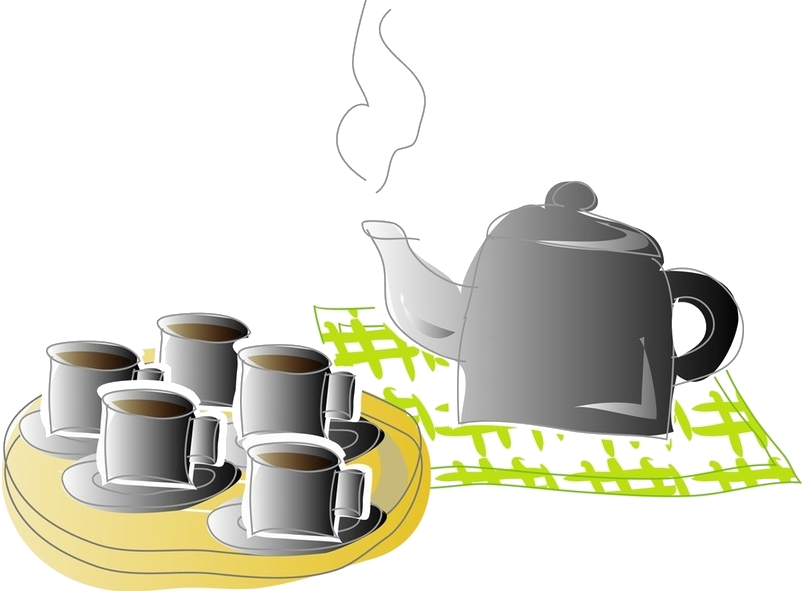
\includegraphics[width=0.75\textwidth]{figure/relax.png}
\end{figure}
\end{frame}

%\section{ XSLT}

\begin{frame}[fragile]{CH7 XSLT}
\begin{figure}
    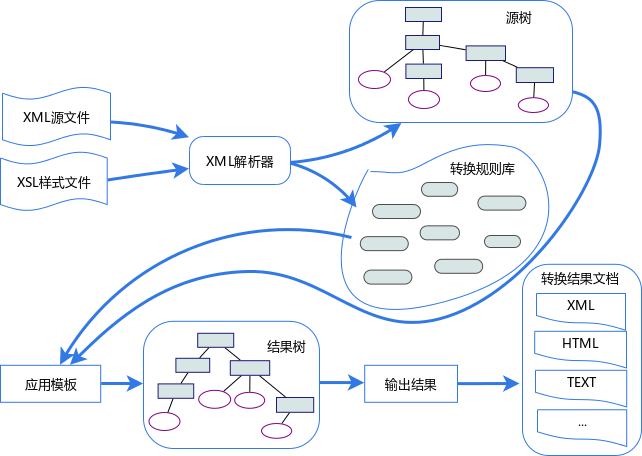
\includegraphics[width=0.9\textwidth]{figure/xslt.png}
\end{figure}
\end{frame}

\begin{frame}[fragile]{本章学习目标}
\begin{easylist} \easyitem
& 了解XSLT的发展历史、XSLT与XSL的关系
& 掌握XSLT的转换处理过程
& 掌握XSLT的基本语法
& 能够使用SAXON进行XSLT测试
\end{easylist}
\end{frame}

\begin{frame}[fragile]{目录}
\begin{easylist} \easyitem
& XSLT概述
& 如何测试XSLT
& XSLT快速入门
& XSLT的输出格式控制
& XSLT的逻辑处理元素
& XSLT的模式
& XSLT的命名模板
& XSLT的函数
& XSLT 2.0
\end{easylist}
\end{frame}


\subsection{7.1 概述}

\begin{frame}[fragile]{7.1 概述}
\begin{easylist} \easyitem
& XSLT与XSL
& XSLT的作用
& XSLT的工作流程
& XSLT的应用模式
& XSLT与CSS的区别
\end{easylist}
\end{frame}


\subsubsection{7.1.1 XSLT与XSL}
\begin{frame}[fragile, allowframebreaks]{7.1.1 XSLT与XSL}
\begin{easylist} \easyitem
& XSLT
&& 可扩展样式语言转换(Extensible Stylesheet Language Transformations)
&& 可扩展样式语言XSL(Extensible Stylesheet Language)的一个组成部分
& XSL
&& 定义XML文档的格式化和呈现方式,以方便在屏幕、纸张等媒介上显示或通过语音输出
&& 包含两个相对独立的阶段:
&&& 结构转换阶段:实现XML文档元素的选择、分组、重新排列
&&& 格式化处理阶段,实现具体的呈现功能

&& XSL又被拆分为两部分:
&&& XSLT用于定义转换
&&& 剩余的部分——仍称为XSL,也有人称之为XSL-FO(XSL Formatting)

&& XSL目前包含三个组成部分
&&& XSL转换XSLT:描述如何把一个XML文档转换为另外一个文本格式的文档,如XML文档或HTML文档
&&& XML路径语言XPath:在XSLT之中实现存取或引用XML文档特定部分的表达式语言
&&& XSL格式化对象(XSL Formatting Objects, XSL-FO):定义XML文档的格式化显示方式
\end{easylist}
\end{frame}


\subsubsection{7.1.2 XSLT的作用}
\begin{frame}[fragile]{7.1.2 XSLT的作用}
\begin{easylist} \easyitem
& 把一个XML文档转换为另一个类型的文档,可以在输出文档里增删元素和属性,可以对源文档的元素进行重新排列,并有选择的组织显示
& 常见的三种转换
\begin{figure}
    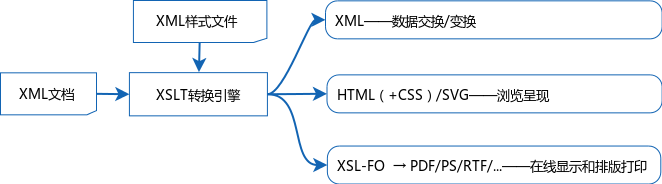
\includegraphics[width=0.85\textwidth]{figure/xslt-transform.png}
\end{figure}
\end{easylist}
\end{frame}


\begin{frame}[fragile]{把一个版本的XML转换为另一个版本}
\begin{lstlisting}[tabsize=8, basicstyle=\small\tt, language=XML]
<v1:order xmlns:v1="http://www.test.com/v1"> 
    <product name="打印纸" price="30" quantity="5"/>
</v1:order>
\end{lstlisting}

\begin{lstlisting}[tabsize=8, basicstyle=\small\tt, language=XML]
<v2:order xmlns:v2="http://www.test.com/v2">
    <product quantity="5">
        <name>打印纸</name>
        <price>30</price>
    </product>
</v2:order>
\end{lstlisting}
\end{frame}


\begin{frame}[fragile]{把XML转换为HTML}
\begin{lstlisting}[tabsize=8, basicstyle=\small\tt, language=HTML]
<html>
    <head><title>Order Details</title></head>
    <body>
        <p>名称:打印纸</p>
        <p>单价:30元;数量:5 </p>
    </body>
</html>
\end{lstlisting}
\end{frame}


\subsubsection{7.1.3 XSLT的工作流程}
\begin{frame}[fragile]{7.1.3 XSLT的工作流程}
\begin{easylist} \easyitem
\begin{figure}
    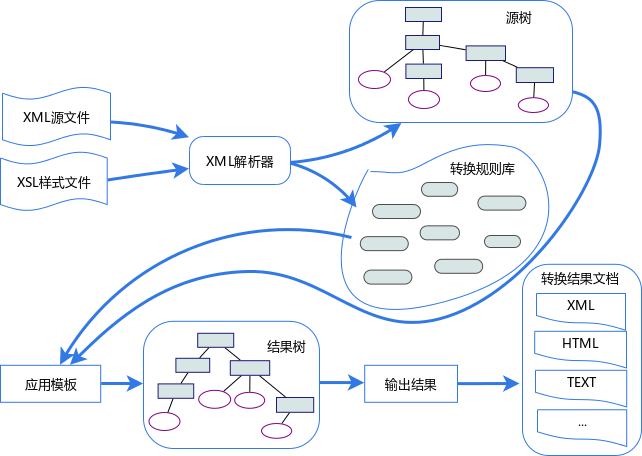
\includegraphics[width=0.75\textwidth]{figure/xslt.png}
\end{figure}
\end{easylist}
\end{frame}


\subsubsection{7.1.4 XSLT的应用模式}
\begin{frame}[fragile]{7.1.4 XSLT的应用模式}
\begin{easylist} \easyitem
& 服务器端应用模式
&& 转换是在服务器端完成
& 客户端应用模式
&& 转换由客户端的浏览器完成
& 独立模式
&& 转换由独立程序完成,如Saxon
\end{easylist}
\end{frame}


\subsubsection{7.1.5 XSLT与CSS的区别}
\begin{frame}[fragile]{7.1.5 XSLT与CSS的区别}
\begin{easylist} \easyitem
& 转换动作不同
&& XSLT采用转换方式,把XML文档由一种格式转换为另一种格式;CSS无转换动作,只是针对XML元素设定显示样式。
& 互动性不同
&& CSS可以实现闪烁等动态效果,XSLT转换本身则没有这方面的功能。
& 语法不同
&& XSL样式文件为标准的XML文件,而CSS的语法自成一格
\end{easylist}
\end{frame}



\subsection{7.2 如何测试XSLT}

\begin{frame}[fragile]{7.2 如何测试XSLT}
\begin{easylist} \easyitem
& 浏览器
& XML工具
& 独立的XSLT处理器
\end{easylist}
\end{frame}


\subsubsection{7.2.1 通过浏览器测试XSLT}
\begin{frame}[fragile]{7.2.1 通过浏览器测试XSLT}
\begin{easylist} \easyitem
& 在XML文档中通过<?xml-stylesheet?>处理指令进行样式的关联
& 通过浏览器打开XML文档查看转换效果
& 看不到转换结果的源代码
\end{easylist}
\end{frame}


\subsubsection{7.2.2 通过XML专业工具测试}
\begin{frame}[fragile]{7.2.2 通过XML专业工具测试}
\begin{figure}
    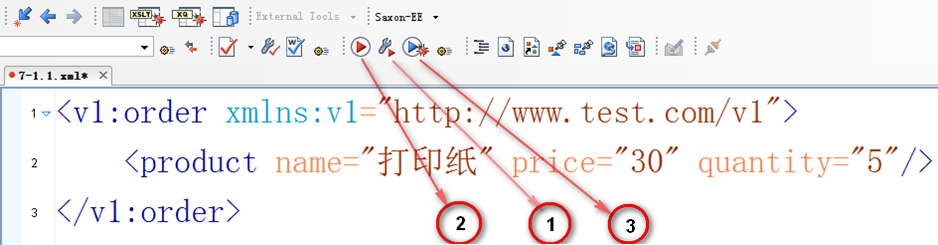
\includegraphics[width=0.85\textwidth]{figure/xslt-oxygen-test.png}
\end{figure}
\end{frame}


\subsubsection{7.2.3 通过XSLT处理器测试}
\begin{frame}[fragile]{7.2.2 通过XSLT处理器测试}
\begin{easylist} \easyitem
& Saxon
&& 安装Java
&& 下载并配置Saxon
&& 指定参数实现样式转换
&&& 语法:
&&&& java -jar saxon9he.jar -s:source -xsl:stylesheet -o:output
&&& 例子:
&&&& java -jar saxon9he.jar -s:7-1.1.xml -xsl:7-1.2.xsl -o:7-1.out.xml
\end{easylist}
\end{frame}


\subsection{7.3 XSLT快速入门}

\begin{frame}[fragile, allowframebreaks]{7.3 XSLT快速入门}
\begin{lstlisting}[tabsize=8, basicstyle=\small\tt, language=XML, caption="7-2.xml"]
<?xml version="1.0"?>
<books>
    <provider>Summer</ provider>
    <book isbn="978-7-115-21703-5">
        <title>Python高级编程</title>
        <price>45.00</price>
        <authors>
            <author>Tarek Ziade</author>
            <author type="translator">姚军</author>
            <author type="translator">夏海伦</author>
            <author type="translator">王秀丽</author>
        </authors>
        <press>人民邮电出版社</press>
        <pages>306</pages>
        <description>介绍了Python语言的最佳实践和敏捷开发方法…</description>
        <cover>book-python.jpg</cover>
    </book>
    <book isbn="978-7-115-28282-8">
        <title>数学之美</title>
        <price>45.00</price>
        <authors>
            <author>吴军</author>
        </authors>
        <press>人民邮电出版社</press>
        <pages>304</pages>
        <description>读了“数学之美”,才发现大学时学的数学知识…</description>
        <cover>book-math.jpg</cover>
    </book>
    <book isbn="978-7-5641-1139-7">
        <title>集体智慧编程(影印版)</title>
        <price>58.00</price>
        <authors>
            <author>Toby Segaran</author>
        </authors>
        <press>东南大学出版社</press>
        <pages>334</pages>
        <description>Toby的书非常成功地将复杂的机器学习算法问题…</description>
        <cover>book-collective.jpg</cover>
    </book>
</books>
\end{lstlisting}

\begin{lstlisting}[tabsize=8, basicstyle=\small\tt, language=XML, caption="7-2.xsl"]
<?xml version="1.0" encoding="UTF-8"?>
<xsl:stylesheet xmlns:xsl="http://www.w3.org/1999/XSL/Transform" version="2.0">
    <xsl:template match="/">
    <html>
        <head><title>图书列表</title></head>
        <body>
            <xsl:apply-templates/>
        </body>
    </html>
    </xsl:template>
    <xsl:template match="books">
        <table>
            <xsl:apply-templates select="book"/>
        </table>
    </xsl:template>
    <xsl:template match="book">
        <tr>
            <td><xsl:value-of select="title"/></td>
        </tr>
    </xsl:template>
</xsl:stylesheet>
\end{lstlisting}

\begin{shaded}
java -jar saxon9he.jar -s:7-2.xml -xsl:7-2.xsl -o:7-2.out.html
\end{shaded}


\begin{lstlisting}[tabsize=8, basicstyle=\small\tt, language=HTML, caption="7-2.out.html"]
<html>
    <head>
        <meta http-equiv="Content-Type" content="text/html; charset=UTF-8">
        <title>图书列表</title>
    </head>
    <body>
        <table>
            <tr><td>Python高级编程</td></tr>
            <tr><td>数学之美</td></tr>
            <tr><td>集体智慧编程(影印版)</td></tr>
        </table>
    </body>
</html>
\end{lstlisting}

\begin{shaded}
利用<?xml-stylesheet?>处理指令在“7-2.xml”中建立与“7-2.xsl”的关联,通过浏览器查看结果
\end{shaded}

\begin{figure}
    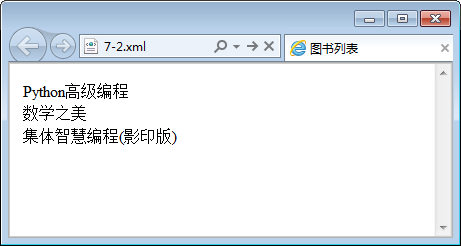
\includegraphics[width=0.75\textwidth]{figure/xslt-7-2.out.png}
\end{figure}
\end{frame}


\subsubsection{7.3.1 stylesheet元素}
\begin{frame}[fragile]{7.3.1 stylesheet元素}
\begin{lstlisting}[tabsize=8, basicstyle=\small\tt, language=XML, numbers=none]
<xsl:stylesheet xmlns:xsl="http://www.w3.org/1999/XSL/Transform" version="2.0">
\end{lstlisting}
\end{frame}


\subsubsection{7.3.2 template元素}
\begin{frame}[fragile]{7.3.2 template元素}
\begin{lstlisting}[tabsize=8, basicstyle=\small\tt, language=XML, numbers=none]
<xsl:template match="要匹配的模式串"
            name="名称"
            priority="代表优先级的数字">
    <!—模板的具体内容 -->
</xsl:template>
\end{lstlisting}
\end{frame}


\subsubsection{7.3.3 apply-templates元素}
\begin{frame}[fragile]{7.3.3 apply-templates元素}
\begin{lstlisting}[tabsize=8, basicstyle=\small\tt, language=XML, numbers=none]
<xsl:template match="/books">
    <xsl:apply-templates select="book "/>
</xsl:template>
\end{lstlisting}

\begin{lstlisting}[tabsize=8, basicstyle=\small\tt, language=XML, numbers=none]
<xsl:template match="/books">
    <xsl:apply-templates/>
</xsl:template>
\end{lstlisting}
\end{frame}


\subsubsection{7.3.4 value-of元素}
\begin{frame}[fragile]{7.3.4 value-of元素}
\begin{easylist} \easyitem
& 根据select属性值从源树中读取信息
& xsl:value-of在XSLT的1.0和2.0版本中转换行为不一致
\begin{lstlisting}[tabsize=8, basicstyle=\small\tt, language=XML, numbers=none]
<xsl:value-of select="author"/>
\end{lstlisting}
&& 在1.0中,仅选取第一个结点的值,结果为:Tarek Ziade
&& 在2.0中,顺序输出所有的结点,默认通过空格分隔:Tarek Ziade 姚军 夏海伦 王秀丽
&& 可更换分隔符,如下:
\begin{lstlisting}[tabsize=8, basicstyle=\small\tt, language=XML, numbers=none]
<xsl:value-of select="author" separator=","/>
\end{lstlisting}
&& 此时结果为:Tarek Ziade,姚军,夏海伦,王秀丽
\end{easylist}
\end{frame}


\subsubsection{7.3.5 attribute元素}
\begin{frame}[fragile]{7.3.5 attribute元素}
\begin{easylist} \easyitem
& 生成属性信息,例如:
\begin{lstlisting}[tabsize=8, basicstyle=\small\tt, language=XML, numbers=none]
<img>
    <xsl:attribute name="src"><xsl:value-of select="cover"/></xsl:attribute>
    <xsl:attribute name="width">80</xsl:attribute>
    <xsl:attribute name="height">100</xsl:attribute>
</img>
\end{lstlisting}
& 结果:
\begin{lstlisting}[tabsize=8, basicstyle=\small\tt, language=HTML, numbers=none]
<img src="book-python.jpg" width="80" height="100"/>
\end{lstlisting}
\end{easylist}
\end{frame}



\subsection{7.4 XSLT的输出格式控制}
\begin{frame}[fragile]{7.4 XSLT的输出格式控制}
\begin{easylist} \easyitem
& 用于指定转换生成的文档格式:
&& XML、HTML、XHTML或纯文本格式
& 例如:声明转换结果的文本为纯文本格式
\begin{lstlisting}[tabsize=8, basicstyle=\small\tt, language=XML, numbers=none]
<xsl:output method="text"/>
\end{lstlisting}
& method的取值:
&& text、xml、xhtml或html
& XSLT 1.0不支持该指令
\end{easylist}
\end{frame}


\subsection{7.5 XSLT的逻辑处理元素}
\begin{frame}[fragile]{7.5 XSLT的逻辑处理元素}
\begin{easylist} \easyitem
& 条件处理元素
&& if
&& choose
& 循环:for-each
& 排序:sort
\end{easylist}
\end{frame}


\subsubsection{7.5.1 条件处理元素}
\begin{frame}[fragile, allowframebreaks]{if元素}
\begin{lstlisting}[tabsize=8, basicstyle=\small\tt, language=XML, caption=样式文档]
<xsl:stylesheet xmlns:xsl="http://www.w3.org/1999/XSL/Transform" version="2.0">
    <xsl:template match="/">
        <html><body>
            <xsl:apply-templates select="books/book"/>
        </body></html>
    </xsl:template>
    <xsl:template match="book">
        <xsl:if test="price &lt; 50">
            <p><xsl:value-of select="title"/></p>
        </xsl:if>
    </xsl:template>
</xsl:stylesheet>
\end{lstlisting}

\begin{lstlisting}[tabsize=8, basicstyle=\small\tt, language=HTML, caption=转换结果]
<html>
    <body>
        <p>Python高级编程</p>
        <p>数学之美</p>
    </body>
</html>
\end{lstlisting}
\end{frame}


\begin{frame}[fragile, allowframebreaks]{choose元素}
\begin{lstlisting}[tabsize=8, basicstyle=\small\tt, language=XML, caption=样式文档]
<xsl:stylesheet xmlns:xsl="http://www.w3.org/1999/XSL/Transform" version="2.0">
    <xsl:template match="/">
        <html><body>
            <xsl:apply-templates select="books/book"/>
        </body></html>
    </xsl:template>
    <xsl:template match="book">
        <xsl:choose>
            <xsl:when test="price &lt; 50"><p><xsl:value-of select="title"/></p></xsl:when>
            <xsl:when test="price &lt; 100"><p>* <xsl:value-of select="title"/></p></xsl:when>
            <xsl:otherwise><p># <xsl:value-of select="title"/></p></xsl:otherwise>
        </xsl:choose>
    </xsl:template>
</xsl:stylesheet>
\end{lstlisting}

\begin{lstlisting}[tabsize=8, basicstyle=\small\tt, language=HTML, caption=转换结果]
<html>
    <body>
        <p>Python高级编程</p>
        <p>数学之美</p>
        <p>*集体智慧编程(影印版)</p>
    </body>
</html>
\end{lstlisting}
\end{frame}


\subsubsection{7.5.2 循环元素for-each}
\begin{frame}[fragile, allowframebreaks]{for-each元素}
\begin{lstlisting}[tabsize=8, basicstyle=\small\tt, language=XML, caption=样式文档]
<xsl:stylesheet xmlns:xsl="http://www.w3.org/1999/XSL/Transform" version="2.0">
    <xsl:template match="/">
        <html><body>
            <xsl:apply-templates select="books"/>
        </body></html>
    </xsl:template>
    <xsl:template match="books">
        <xsl:for-each select="book">
            <p><xsl:value-of select="title"/></p>
        </xsl:for-each>
    </xsl:template>
</xsl:stylesheet>
\end{lstlisting}

\begin{lstlisting}[tabsize=8, basicstyle=\small\tt, language=HTML, caption=转换结果]
<html>
    <body>
        <p>Python高级编程</p>
        <p>数学之美</p>
        <p>集体智慧编程(影印版)</p>
    </body>
</html>
\end{lstlisting}
\end{frame}


\subsubsection{7.5.3 排序元素sort}
\begin{frame}[fragile, allowframebreaks]{sort元素}
\begin{lstlisting}[tabsize=8, basicstyle=\small\tt, language=XML, caption=样式文档]
<xsl:stylesheet xmlns:xsl="http://www.w3.org/1999/XSL/Transform" version="2.0">
    <xsl:template match="/">
        <html><body>
            <xsl:apply-templates select="books"/>
        </body></html>
    </xsl:template>
    <xsl:template match="books">
        <xsl:for-each select="book">
            <xsl:sort select="price" order="descending"/>
            <p><xsl:value-of select="title"/></p>
        </xsl:for-each>
    </xsl:template>
</xsl:stylesheet>
\end{lstlisting}

\begin{lstlisting}[tabsize=8, basicstyle=\small\tt, language=HTML, caption=转换结果]
<html>
    <body>
        <p>集体智慧编程(影印版)</p>
        <p>Python高级编程</p>
        <p>数学之美</p>
    </body>
</html>
\end{lstlisting}
\end{frame}



\subsection{7.6 XSLT的模式-mode}
\begin{frame}[fragile, allowframebreaks]{7.6 XSLT的模式-mode}
\begin{lstlisting}[tabsize=8, basicstyle=\small\tt, language=XML, caption=样式文档]
<xsl:stylesheet xmlns:xsl="http://www.w3.org/1999/XSL/Transform" version="2.0">
    <xsl:template match="/">
        <html><body>
            <h2>按照价格降序排列的图书名称</h2>
            <xsl:apply-templates select="books" mode="simple"/>
            <h2>图书详细列表</h2>
            <xsl:apply-templates select="books" mode="detail"/>
        </body></html>
    </xsl:template>
    <xsl:template match="books" mode="simple">
        <ul>
            <xsl:for-each select="book">
                <xsl:sort select="price" order="descending"/>
                <li><xsl:value-of select="title"/></li>
            </xsl:for-each>
        </ul>
    </xsl:template>
    
    <xsl:template match="books" mode="detail">
        <table>
            <tr>
                <td>ISBN</td><td>标题</td><td>作者</td><td>出版社</td><td>价格</td>
            </tr>
            <xsl:for-each select="book">
                <xsl:sort select="pages" order="ascending"/>
                <tr>
                    <td><xsl:value-of select="@isbn"/></td>
                    <td><xsl:value-of select="title"/></td>
                    <td><xsl:value-of select="authors"/></td>
                    <td><xsl:value-of select="press"/></td>
                    <td><xsl:value-of select="price"/></td>
                    <td><img><xsl:attribute name="src" select="cover"/></img></td>
                </tr>
            </xsl:for-each>
        </table>
    </xsl:template>
</xsl:stylesheet>
\end{lstlisting}

\begin{lstlisting}[tabsize=8, basicstyle=\small\tt, language=HTML, caption=转换结果]
<html>
    <body>
        <h2>按照价格降序排列的图书名称</h2>
        <ul>
            <li>集体智慧编程(影印版)</li>
            <li>Python高级编程</li>
            <li>数学之美</li>
        </ul>
        <h2>图书详细列表</h2>
        <table>
            <tr>
                <td>ISBN</td><td>标题</td><td>作者</td><td>出版社</td><td>价格</td>
            </tr>
            <tr>
                <td>978-7-115-28282-8</td>
                <td>数学之美</td>
                <td>吴军</td>
                <td>人民邮电出版社</td>
                <td>45.00</td>
                <td><img src="book-math.jpg"></td>
            </tr>
            <tr>
                <td>978-7-115-21703-5</td>
                <td>Python高级编程</td>
                <td>Tarek Ziade 姚军 夏海伦 王秀丽</td>
                <td>人民邮电出版社</td>
                <td>45.00</td>
                <td><img src="book-python.jpg"></td>
            </tr>
            <tr>
                <td>978-7-5641-1139-7</td>
                <td>集体智慧编程(影印版)</td>
                <td>Toby Segaran</td>
                <td>东南大学出版社</td>
                <td>58.00</td>
                <td><img src="book-collective.jpg"></td>
            </tr>
        </table>
    </body>
</html>
\end{lstlisting}
\end{frame}



\subsection{7.7 XSLT的命名模版}
\begin{frame}[fragile, allowframebreaks]{7.7 XSLT的命名模版}
\begin{easylist} \easyitem
& 模版定义语法:
\begin{lstlisting}[tabsize=8, basicstyle=\small\tt, language=XML, numbers=none]
<xsl:template name="模板名称">
    <!—模板的具体内容 -->
</xsl:template>
\end{lstlisting}
& 定义好的模板通过xsl:call-template指令进行调用
& 示例:
\end{easylist}
\begin{lstlisting}[tabsize=8, basicstyle=\small\tt, language=XML, caption=样式文档]
<xsl:stylesheet xmlns:xsl="http://www.w3.org/1999/XSL/Transform" version="2.0">
    <xsl:template match="/">
        <html><body>
            <h2>图书提供者信息</h2>
            <xsl:call-template name="providerTemplate"/>
            <h2>按照价格降序排列的图书名称</h2>
            <xsl:apply-templates select="books" mode="simple"/>
            <h2>图书详细列表</h2>
            <xsl:apply-templates select="books" mode="detail"/>
        </body></html>
    </xsl:template>
    
    <xsl:template name="providerTemplate">
        <p>本图书列表由:
        <strong><xsl:value-of select="/books/provider"/></strong>提供.
        </p>
    </xsl:template>
    
    <xsl:template match="books" mode="simple">
        <!-- 省略,同7-7.xsl对应内容… -->
    </xsl:template>
    
    <xsl:template match="books" mode="detail">
        <!-- 省略,同7-7.xsl对应内容… -->
    </xsl:template>
</xsl:stylesheet>
\end{lstlisting}

\begin{lstlisting}[tabsize=8, basicstyle=\small\tt, language=HTML, caption=转换结果]
<html>
    <body>
        <h2>图书提供者信息</h2>
        <p>本图书列表由:<strong>Summer</strong>提供. </p>
        <h2>按照价格降序排列的图书名称</h2>
        <!-- 以下内容与7-7.out.html相同,此处省略… -->
    </body>
</html>
\end{lstlisting}
\end{frame}



\subsection{7.8 XSLT的函数}
\begin{frame}[fragile, allowframebreaks]{7.8 XSLT的函数}
\begin{easylist} \easyitem
& 可以直接使用XPath的函数
& XSLT本身的函数
&& document()
&& key()
&& format-number()
&& generate-id()
& 示例:
\end{easylist}
\begin{lstlisting}[tabsize=8, basicstyle=\small\tt, language=XML, caption=样式文档]
<xsl:stylesheet xmlns:xsl="http://www.w3.org/1999/XSL/Transform" version="2.0">
    <xsl:template match="/">
        <html><body>
            <h2>图书平均价格信息</h2>
            <xsl:call-template name="priceTemplate"/>
        </body></html>
    </xsl:template>
    <xsl:template name="priceTemplate">
    平均价格:
    <xsl:value-of select="format-number(sum(/books/book/price) div count(/books/book/price), '0')"/>
    </xsl:template>
</xsl:stylesheet>
\end{lstlisting}

\begin{lstlisting}[tabsize=8, basicstyle=\small\tt, language=HTML, caption=转换结果]
<html>
    <body>
        <h2>图书平均价格信息</h2>
        平均价格:49
    </body>
</html>
\end{lstlisting}
\end{frame}


\subsection{7.9 XSLT 2.0新特性}
\begin{frame}[fragile]{7.9 XSLT 2.0新特性}
\begin{easylist} \easyitem
& 新增数据模型
& 支持Schema数据类型
& 新增元素和函数
& 支持非XML输入源
& 改进了字符处理
& 支持多文件输出
\end{easylist}
\end{frame}



\begin{frame}
\begin{center}
    \Huge END
\end{center}
\begin{figure}
    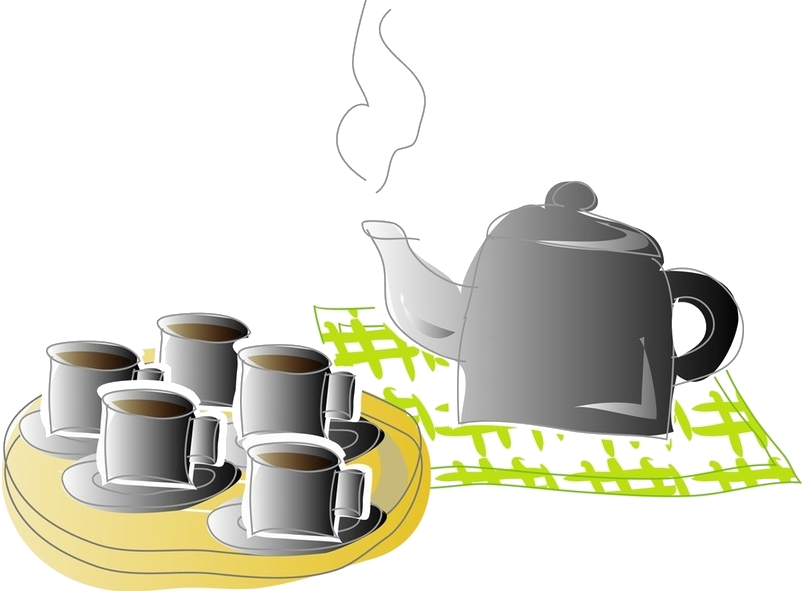
\includegraphics[width=0.75\textwidth]{figure/relax.png}
\end{figure}
\end{frame}

%\section{ JavaScript}

\begin{frame}[fragile]{CH8 JavaScript}
\begin{figure}
    
\includegraphics[width=0.9\textwidth]{figure/javascript.jpg}
\end{figure}
\end{frame}

\begin{frame}[fragile]{本章学习目标}
\begin{easylist} \easyitem
& 了解JavaScript的起源
& 掌握JavaScript的测试方法
& 熟悉JavaScript的基本语法,能借助于文档进行基本的脚本编写
& 了解浏览器对象模型BOM
& 理解JavaScript的定时器操作
\end{easylist}
\end{frame}

\begin{frame}[fragile]{目录}
\begin{easylist} \easyitem
& JavaScript概述
& JavaScript的测试方法
& JavaScript的变量和常量
& JavaScript的基本语句
& 函数和数组
& 对象
& 浏览器对象模型BOM
& 定时器
\end{easylist}
\end{frame}


\subsection{8.1 JavaScript概述}

\begin{frame}[fragile]{8.1 JavaScript概述}
\begin{easylist} \easyitem
& 1995年 $\rightarrow$ Brendan Eich $\rightarrow$ 网景公司  $\rightarrow$ JavaScript
& JavaScript vs Applet
& JavaScript vs JScript
& 当前JavaScript的三大组成部分
&& ECMAScript语言核心
&& DOM(Document Object Model)文档对象模型
&& BOM(Browser Object Model)浏览器对象模型
\end{easylist}
\end{frame}


\begin{frame}[fragile]{jQuery}
\begin{easylist} \easyitem
& JavaScript的跨浏览器问题
& jQuery解决方案
&& John Resig创建的一个轻量级JavaScript库
&& 充分利用了CSS的优势,支持扩展,能够抽象浏览器的不一致性,并支持隐式迭代和连缀操作
\end{easylist}
\end{frame}


\begin{frame}[fragile, allowframebreaks]{jQuery}
\begin{easylist} \easyitem
& 下载使用
\begin{figure}
    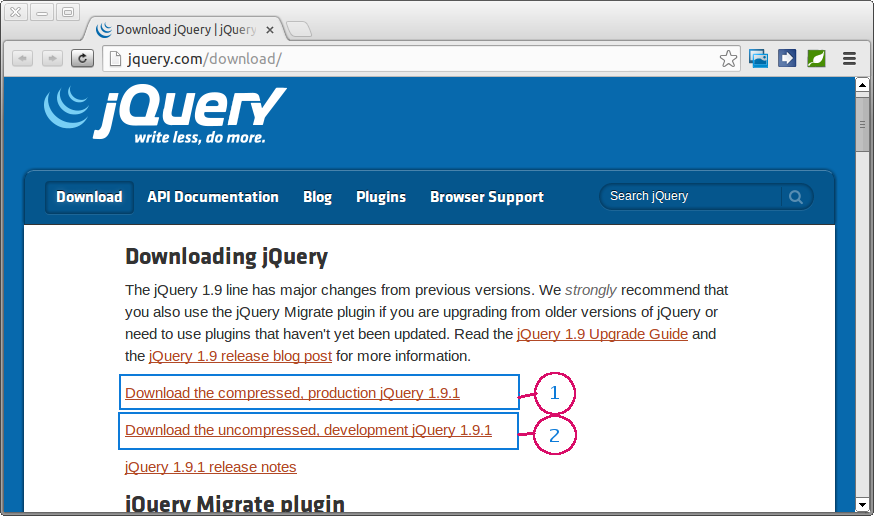
\includegraphics[width=0.75\textwidth]{figure/js-jquery.png}
\end{figure}
\newpage
& 嵌入方法
\begin{lstlisting}[tabsize=8, basicstyle=\small\tt, language=JavaScript, numbers=none]
<script type="text/javascript" src="jquery.js"></script>
\end{lstlisting}
& 使用托管版本
\begin{lstlisting}[tabsize=8, basicstyle=\small\tt, language=JavaScript, numbers=none]
<script type="text/javascript" 
src=" http://ajax.googleapis.com/ajax/libs/jquery/1.9.1/jquery.min.js "></script>
\end{lstlisting}
\end{easylist}
\end{frame}



\subsection{8.2 JavaScript的测试方法}

\begin{frame}[fragile]{8.2 JavaScript的测试方法}
\begin{easylist} \easyitem
& 与网页的关联测试方法
& 在页面加载之后运行JavaScript
& 浏览器内置的JavaScript控制台
\end{easylist}
\end{frame}


\subsubsection{8.2.1 与网页的关联测试方法}
\begin{frame}[fragile]{8.2.1 与网页的关联测试方法}
\begin{easylist} \easyitem
& 编写JavaScript脚本文件,并保存到以.js结尾的文件中,然后通过HTML语言中script标记的src属性进行关联
& 在<script>标记的开始和结束之间,直接嵌入JavaScript脚本
& 考虑二者的优缺点
\end{easylist}
\end{frame}


\begin{frame}[fragile]{示例}
\begin{lstlisting}[tabsize=8, basicstyle=\small\tt, language=HTML]
<html>
    <head>
        <title>JavaScript DEMO</title>
        <script type="text/javascript" src="jquery.js"></script>
        <script type="text/javascript">
            $(document).ready(function() {
                alert('hello world');
            });
        </script>
    </head>
    <body>
        <h1>JavaScript Test</h1>
    </body>
</html>
\end{lstlisting}
\end{frame}


\subsubsection{8.2.2 在页面加载之后运行JavaScript}
\begin{frame}[fragile]{8.2.2 在页面加载之后运行JavaScript}
\begin{easylist} \easyitem
& JavaScript默认在网页中的添加位置立即加载运行
&& 问题
&& 难度
& jQuery的实现方式
\begin{lstlisting}[tabsize=8, basicstyle=\small\tt, language=JavaScript, numbers=none]
$(document).ready(function() {
    //将想在网页加载完毕后再运行的代码放在此处…
});
\end{lstlisting}
\end{easylist}
\end{frame}


\subsubsection{8.2.3 利用浏览器内置的JavaScript控制台}
\begin{frame}[fragile]{8.2.3 利用浏览器内置的JavaScript控制台}
\begin{easylist} \easyitem
& Firefox
&& “Tools” $\rightarrow$ “Web Developer” $\rightarrow$ “Web Console”
&& CTRL+SHIFT+K
& CHROME
&& “Tools” $\rightarrow$ “JavaScript Console”
&& CTRL+SHIFT+J
& OPERA
&& “Developer Tools” $\rightarrow$ “Web Inspector”
&& CTRL+SHIFT+I
& IE
&& “Tools” $\rightarrow$ “F12 Developer Tools”
&& F12
\end{easylist}
\end{frame}


\begin{frame}[fragile]{Google Chrome的JavaScript控制台}
\begin{figure}
    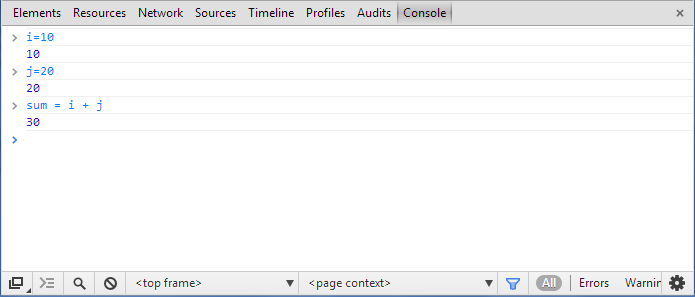
\includegraphics[width=0.9\textwidth]{figure/js-chrome-console.png}
\end{figure}
\end{frame}



\subsection{8.3 JavaScript的变量和常量}

\begin{frame}[fragile]{8.3 JavaScript的变量和常量}
\begin{easylist} \easyitem
& 数据类型
& 变量的声明和赋值
& 变量的作用域
& 常量
\end{easylist}
\end{frame}


\subsubsection{8.3.1 数据类型}
\begin{frame}[fragile]{8.3.1 数据类型}
\begin{figure}
    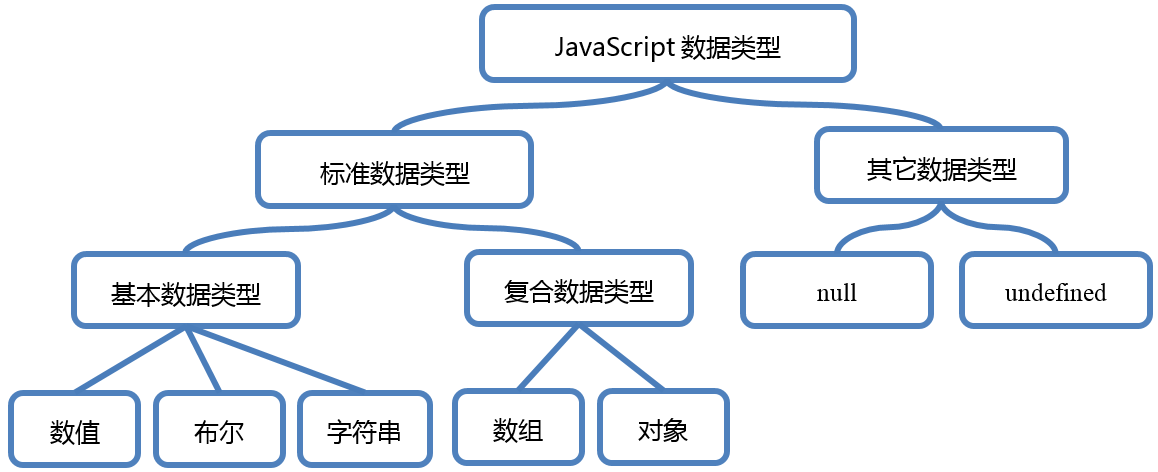
\includegraphics[width=1.0\textwidth]{figure/js-datatype.png}
\end{figure}
\end{frame}


\begin{frame}[fragile]{利用控制台查看数据类型}
\begin{figure}
    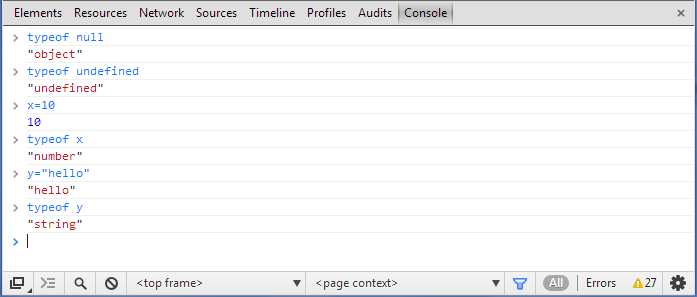
\includegraphics[width=1.0\textwidth]{figure/js-datatype2.png}
\end{figure}
\end{frame}


\subsubsection{8.3.2 变量的声明和赋值}
\begin{frame}[fragile]{8.3.2 变量的声明和赋值}
\begin{easylist} \easyitem
& 变量声明
\begin{lstlisting}[tabsize=8, basicstyle=\small\tt, language=JavaScript, numbers=none]
var userName;
\end{lstlisting}
& 变量赋值
\begin{lstlisting}[tabsize=8, basicstyle=\small\tt, language=JavaScript, numbers=none]
username="李白";
\end{lstlisting}
& 声明和赋值同时进行
\begin{lstlisting}[tabsize=8, basicstyle=\small\tt, language=JavaScript, numbers=none]
var userName="李白";
\end{lstlisting}
\end{easylist}
\end{frame}


\subsubsection{8.3.3 变量的作用域}
\begin{frame}[fragile]{8.3.3 变量的作用域}
\begin{easylist} \easyitem
& 全局变量
&& 在函数之外声明的变量
& 局部变量
&& 在函数之中声明的变量
& 局部变量对全局变量具有覆盖作用
& 考虑以下代码的输出结果:
\begin{lstlisting}[tabsize=8, basicstyle=\small\tt, language=JavaScript]
var a = 6;
function myfunction(){
    var a = 7;
    var b = 8;
    return a+b;
}
console.info(myfunction());
\end{lstlisting}
\end{easylist}
\end{frame}


\subsubsection{8.3.4 常量}
\begin{frame}[fragile]{8.3.4 常量}
\begin{easylist} \easyitem
& 不变的量,用关键字const来声明
\begin{lstlisting}[tabsize=8, basicstyle=\small\tt, language=JavaScript, numbers=none]
const A = 10;
const B = .314;
\end{lstlisting}
& 常量类型
&& 数字常量
&& 非数字NaN(Not A Number)
&& 布尔常量:true、false
&& 字符串
&& 转义字符
&&& $\backslash$b(退格)、$\backslash$f(换页)、$\backslash$n(换行)、$\backslash$r(回车)、$\backslash$t(跳格)、$\backslash$’(单引号)、$\backslash$"(双引号)
\end{easylist}
\end{frame}



\subsection{8.4 JavaScript的基本语句}

\begin{frame}[fragile]{8.4 JavaScript的基本语句}
\begin{easylist} \easyitem
& 注释语句
& 条件语句
& 循环语句
\end{easylist}
\end{frame}


\subsubsection{8.4.1 注释语句}
\begin{frame}[fragile]{8.4.1 注释语句}
\begin{lstlisting}[tabsize=8, basicstyle=\small\tt, language=JavaScript]
//这一行是注释内容
/*这里
*也是注释内容
*/
\end{lstlisting}
\end{frame}


\subsubsection{8.4.2 条件语句}
\begin{frame}[fragile]{8.4.2 条件语句}
\begin{easylist} \easyitem
& 条件运算符
&& 比较运算符
&&& >, >=, <, <=, ==, !=
&& 逻辑运算符
&&& \&\&, ||, !
& if语句
\end{easylist}
\end{frame}


\begin{frame}[fragile]{if语句}
\begin{lstlisting}[tabsize=8, basicstyle=\small\tt, language=JavaScript]
var hour = 20;
if (hour == 20) {
    alert("Now is 20 o’clock.");
}
\end{lstlisting}
\end{frame}


\begin{frame}[fragile, allowframebreaks]{if-else-else if语句}
\begin{lstlisting}[tabsize=8, basicstyle=\small\tt, language=HTML]
<html>
    <head>
        <title>IF DEMO</title>
        <meta http-equiv="Content-Type" content="text/html;charset=utf-8"/>
    </head>
    <body>
        <h1>条件语句测试</h1>
        <script type="text/javascript">
            var d = new Date();  //get current date and time
            var hour = d.getHours();
            var msg;

            if((hour>=7) && (hour<12)) {
                msg = '上午';
            } else if((hour>=12) && (hour<18)){
                msg = '下午';
            } else if((hour>=18) && (hour<22)) {
                msg = '晚上';
            } else {
                msg = '夜间';
            }

            document.write('现在是:' + msg);
        </script>
    </body>
</html>
\end{lstlisting}
\end{frame}


\subsubsection{8.4.3 循环语句}
\begin{frame}[fragile]{8.4.3 循环语句}
\begin{easylist} \easyitem
& for
\begin{lstlisting}[tabsize=8, basicstyle=\small\tt, language=JavaScript, numbers=none]
for (初始变量; 循环条件; 变量更新){
    循环主体语句;
}
\end{lstlisting}
& while
\begin{lstlisting}[tabsize=8, basicstyle=\small\tt, language=JavaScript, numbers=none]
while (循环条件){
    循环主体语句;
}
\end{lstlisting}
& break \& continue
\end{easylist}
\end{frame}


\begin{frame}[fragile, allowframebreaks]{循环语句示例}
\begin{lstlisting}[tabsize=8, basicstyle=\small\tt, language=HTML]
<html>
    <head>
        <title>LOOP DEMO</title>
        <meta http-equiv="Content-Type" content="text/html;charset=utf-8"/>
    </head>
    <body>
        <h1>条件语句测试</h1>
        <script type="text/javascript">
            var i=0, n=30, sum=0;
            var lastNumber = 0;
            while(i < n){
                if(i%2 == 0){
                    i++;
                    continue;
                } else {
                    sum = sum + i;
                    lastNumber = i;
                    i++;
                }
                if(i >= 50) break;
            }
            document.write('1+3+5+...+' + lastNumber + '=' + sum);
        </script>
    </body>
</html>
\end{lstlisting}
\end{frame}


\subsection{8.5 函数和数组}

\begin{frame}[fragile]{8.5 函数和数组}
\begin{easylist} \easyitem
& 函数
& 数组
\end{easylist}
\end{frame}


\subsubsection{8.5.1 函数}
\begin{frame}[fragile, allowframebreaks]{8.5.1 函数}
\begin{easylist} \easyitem
& 创建函数
\begin{lstlisting}[tabsize=8, basicstyle=\small\tt, language=JavaScript, numbers=none]
function 函数名称(参数列表) {
    函数内部的语句段
}
\end{lstlisting}
& 例子
\begin{lstlisting}[tabsize=8, basicstyle=\small\tt, language=JavaScript]
//函数示例1:函数中包括了alert这个内置的弹出警告框函数
function welcome () {
    alert ( "hello,this is a function!");
} 

//函数示例2:对a、b两个参数进行求和,并用return语句返回结果
function sum ( a,b) {
    return a+b;
}
\end{lstlisting}

& 字面量方式创建函数
\begin{lstlisting}[tabsize=8, basicstyle=\small\tt, language=JavaScript, numbers=none]
var变量名称 = function 可选函数名称(函数参数){语句段};
\end{lstlisting}
& 例子
\begin{lstlisting}[tabsize=8, basicstyle=\small\tt, language=JavaScript]
var test = function(){
    alert("hello world");
}
test();
\end{lstlisting}
\end{easylist}
\end{frame}

\begin{frame}[fragile]{函数参数}
\begin{easylist} \easyitem
& 形式参数(形参) vs 实际参数(实参)
&& 形式参数只是一个指代,而真正在调用中起作用的是实参
& 例子
\begin{lstlisting}[tabsize=8, basicstyle=\small\tt, language=JavaScript]
function plus (a,b) { //这里a,b是形式参数
    return a+b;
}
plus (3, 5);  //将两个数字作为实参传入
plus (plus(1,2) ,plus(2,3));  //将两个函数作为实参传入
\end{lstlisting}
& Arguments
\end{easylist}
\end{frame}


\begin{frame}[fragile]{函数调用与返回}
\begin{lstlisting}[tabsize=8, basicstyle=\small\tt, language=JavaScript]
function add (x,y){
    return x+y;
}
alert (add(3,9));
\end{lstlisting}
\end{frame}


\subsubsection{8.5.2 数组}
\begin{frame}[fragile]{8.5.2 数组}
\begin{easylist} \easyitem
& 创建数组
\begin{lstlisting}[tabsize=8, basicstyle=\small\tt, language=JavaScript]
var base = [1,2,3,4,5,6,7,8];
var table = [[1,2,3,4],[5,6,7,8],[9,10,11,12]];  //此处构造了一个二维数组
\end{lstlisting}

& 访问和修改
\begin{lstlisting}[tabsize=8, basicstyle=\small\tt, language=JavaScript]
var base = [1,2,3,4,5,6,7,8,9];
base[0] = 10;
base[1] = 20;
for (var i=0;i<base.length;i++)
    base[i]++;
console.info(base);
\end{lstlisting}
\end{easylist}
\end{frame}



\subsection{8.6 对象}

\begin{frame}[fragile]{8.6 对象}
\begin{easylist} \easyitem
& 创建对象
& 属性和方法
& 基本类型和引用类型
& 原型与继承
& 类方法
\end{easylist}
\end{frame}


\subsubsection{8.6.1 创建对象}
\begin{frame}[fragile]{8.6.1 创建对象}
\begin{easylist} \easyitem
& 对象类型
&& Object
&& Function(函数对象)
&& Array(数组对象)
&& Date
&& Math
&& RegExp(正则表达式)
&& Error(错误)
&& 字符串、布尔、数值的包装对象:String、Boolean、Number
\end{easylist}
\end{frame}


\begin{frame}[fragile]{通过new构造对象}
\begin{lstlisting}[tabsize=8, basicstyle=\small\tt, language=JavaScript]
var num=new Object();//自定义一个Object对象的实例并命名为num
num.x=1;
num.y=2;  //为num对象设置两个属性x和y,并分别赋值为1和2
var z=new Array(3);  //定义一个长度为3的数组对象z
var a=new Array (1,2,3,4); //定义一个数组对象a并设定前4个元素为1、2、3、4
var b=new function(){
    alert("hello world");
}  //定义一个函数对象b
\end{lstlisting}
\end{frame}


\begin{frame}[fragile]{通过字面量构造对象}
\begin{lstlisting}[tabsize=8, basicstyle=\small\tt, language=JavaScript]
obj_1 = {
    x: "h1",
    y: function () {
        alert("Hello world!");
    }
};
obj_2 = {
    z: [1,2,3,4],
    add: function(a,b) {
        return a+b;
    }
};
\end{lstlisting}
\end{frame}



\subsubsection{8.6.2 属性和方法}
\begin{frame}[fragile]{8.6.2 属性和方法}
\begin{lstlisting}[tabsize=8, basicstyle=\small\tt, language=JavaScript]
var obj = {};
obj.color = "red";
obj.text = "hello";
obj.work = function(worker){
    console.info(worker + " is working!");
};
\end{lstlisting}
\end{frame}


\subsubsection{8.6.3 基本类型和引用类型}
\begin{frame}[fragile, allowframebreaks]{8.6.3 基本类型和引用类型}
\begin{easylist} \easyitem
& 基本类型
&& 指数值、字符串、布尔值等这类原始值
& 引用类型
&& 指对象类型
\newpage
& 例子
\begin{lstlisting}[tabsize=8, basicstyle=\small\tt, language=JavaScript]
var a = 6;
var b = a;
var b = 7;//此时b的值为7,a的值仍为6
console.info("a=" + a + ", b=" + b);
var oneday= new Date (2050,1,1);
var c = oneday;
c.setDate(11);
oneday.getDate();//此时变量c和oneday的日期的天数均变为11
console.info("oneday.getDate()=" + oneday.getDate() + ", c.getDate()=" + c.getDate());
\end{lstlisting}
&& 思考:输出结果为?
\end{easylist}
\end{frame}


\subsubsection{8.6.4 原型与继承}
\begin{frame}[fragile, allowframebreaks]{8.6.4 原型与继承}
\begin{easylist} \easyitem
& JavaScript借助于原型(prototype)实现继承
&& 把prototype看作是一个模版,新创建的自定义对象则是这个模版(prototype)的一个拷贝
& 例子
\begin{lstlisting}[tabsize=8, basicstyle=\small\tt, language=JavaScript]
function Animal(name, age) {
    this.name = name;
    this.age = age;
}
Animal.prototype = {
    getName: function(){
        return this.name;
    },
    getAge: function(){
        return this.age;
    }
}
var tom = new Animal("Tom Cat", 2);
console.info(tom.getName() + " is " + tom.getAge() + " years old.");
\end{lstlisting}
& 每一个对象都有相应的原型
& prototype属性默认初始化为一个对象
\end{easylist}
\end{frame}



\subsubsection{8.6.5 类方法}
\begin{frame}[fragile, allowframebreaks]{8.6.5 类方法}
\begin{easylist} \easyitem
& 实例方法、原型方法和类方法
& 例子
\begin{lstlisting}[tabsize=8, basicstyle=\small\tt, language=JavaScript]
function Animal(name) {
    this.name=name;
    //以下定义的introduce 为实例方法
    this.introduce=function(){
        console.info("I am " + this.name);
    }
}

//类方法
Animal.run = function(){
    console.info("I can run");
}

//原型方法
Animal.prototype.introduceInChinese=function(){
    console.info("我是"+this.name);
}

//测试
var tom =new Animal("Tom Cat");
tom.introduce();
Animal.run(); //注意:类方法只能通过类名称调用,不能通过实例调用,如tom.run()
tom.introduceInChinese();
\end{lstlisting}
\end{easylist}
\end{frame}



\subsection{8.7 浏览器对象模型BOM}

\begin{frame}[fragile]{8.7 浏览器对象模型BOM}
\begin{easylist} \easyitem
& \em{Widow}
& \em{Document}
& Navigator
& Location
& Screen
& History
\end{easylist}
\end{frame}


\begin{frame}[fragile]{Window}
\begin{easylist} \easyitem
& window是全局对象,每个窗口(包括浏览器窗口和框架窗口)都对应于一个Window对象
& 引用方式
&& window.属性名称或方法名
&& 当访问当前窗口的window对象,可以省略window
&& window对象是代码在浏览器中解释时的全局对象,当运行环境不是浏览器时,window对象不存在
\end{easylist}
\end{frame}


\begin{frame}[fragile]{常见的Window对象的属性和方法}
\begin{table}[!hbp] 
\begin{tabular}{l|l}
\Xhline{1.3pt}
属性/方法名称 & 描述  \\ \Xhline{1.3pt}
document & 返回浏览器内置的Document对象 \\ \hline
navigator & 返回浏览器内置的Navigator对象 \\ \hline
location & 返回浏览器内置的Location对象 \\ \hline
history & 返回浏览器内置的History对象 \\ \hline
screen & 返回浏览器内置的Screen对象 \\ \hline
name & 设置或返回窗口的名称 \\ \hline
open() & 创建一个新的浏览器窗并载入指定的url \\ \hline
close() & 关闭一个浏览器窗口 \\ \hline
alert() & 弹出一个消息框 \\ \hline
confirm() & 弹出一个确认框 \\ \hline
prompt() & 弹出一个提示框 \\ \hline
\end{tabular}
\end{table}
\end{frame}


\begin{frame}[fragile]{常见的Document对象的属性和方法}
\begin{table}[!hbp] 
\begin{tabular}{l|l}
\Xhline{1.3pt}
属性/方法名称 & 描述  \\ \Xhline{1.3pt}
body & 访问文档的body元素 \\ \hline
domain & 返回当前文档的域名 \\ \hline
title & 返回当前文档的标题 \\ \hline
URL & 返回当前文档的URL \\ \hline
referrer & 返回载入当前文档的原文档的URL \\ \hline
getElementById() & 返回对拥有指定 id 的第一个对象的引用 \\ \hline
getElementsByTagName() & 返回带有指定标签名称的对象集合 \\ \hline
write() & 向当前文档写入HTML表达式或JS代码 \\ \hline
writeln() & 等同于write(),但在输出后会添加换行符 \\ \hline
\end{tabular}
\end{table}
\end{frame}


\begin{frame}[fragile]{练习}
\begin{easylist} \easyitem
& 通过JavaScript控制台获取网页http://www.ruc.edu.cn/中的所有链接
\end{easylist}
\end{frame}



\subsection{8.8 定时器}

\begin{frame}[fragile]{8.8 定时器}
\begin{easylist} \easyitem
& 一次性定时器
&& 设置:setTimeout(f, milliseconds);
&& 取消:clearTimeout(timer);
& 重复定时器
&& 设置:setInterval(f, milliseconds);
&& 取消:clearInterval(timer);
\end{easylist}
\end{frame}

\begin{frame}[fragile]{定时器示例}
\begin{lstlisting}[tabsize=8, basicstyle=\small\tt, language=HTML]
<html>
    <head>
        <title>setTimeout DEMO</title>
        <script type="text/javascript" src="jquery.js"></script>
        <script type="text/javascript">
            $(document).ready(function() {
                function onTimer( ){
                    alert("DING DING");
                };
                var timer = setTimeout(onTimer, 2000);
            });
        </script>
    </head>
    <body>
        <h1>setTimeout DEMO</h1>
    </body>
</html>
\end{lstlisting}
\end{frame}



\begin{frame}
\begin{center}
    \Huge END
\end{center}
\begin{figure}
    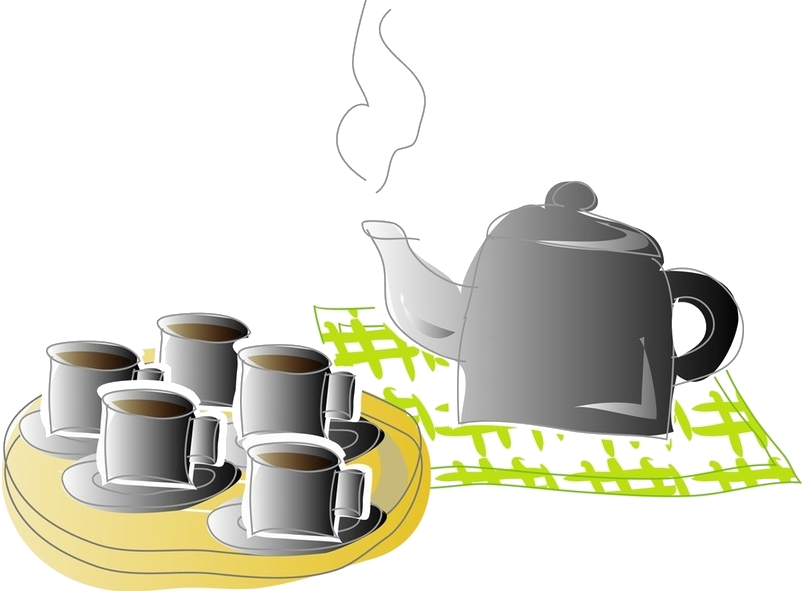
\includegraphics[width=0.75\textwidth]{figure/relax.png}
\end{figure}
\end{frame}

%\section{ DOM}

\begin{frame}[fragile]{CH9 文档对象模型DOM}
\begin{figure}
    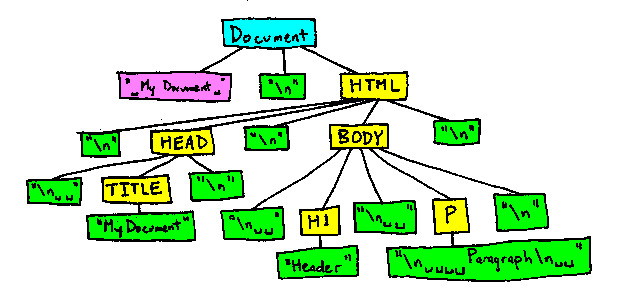
\includegraphics[width=0.9\textwidth]{figure/dom.png}
\end{figure}
\end{frame}

\begin{frame}[fragile]{本章学习目标}
\begin{easylist} \easyitem
& 了解DOM的特点及规范级别
& 掌握常见的DOM对象
& 熟悉浏览器操纵HTML文档和XML文档的基本方法
\end{easylist}
\end{frame}

\begin{frame}[fragile]{目录}
\begin{easylist} \easyitem
& DOM概述
& DOM基本对象
& 利用Mongoose搭建DOM测试环境
& 利用DOM操纵HTML
& 利用DOM操纵XML
\end{easylist}
\end{frame}


\subsection{9.1 DOM概述}

\begin{frame}[fragile]{9.1 DOM概述}
\begin{easylist} \easyitem
& DOM——Document Object Model
&& 文档对象模型的缩写,把整个XML文档表示成一棵由结点组成的层次树,方便人们通过编程语言进行操纵处理
&& 面向程序员实现对XML的操纵处理
\end{easylist}
\end{frame}


\begin{frame}[fragile]{DOM的优点}
\begin{easylist} \easyitem
& DOM优点
&& DOM以易于程序员理解的结点树表示XML文档,简化了文档操作
&& DOM提供了语言中立的标准接口,降低了学习和交流成本
& 其他处理技术
&& SAX:Simple API for XML
&& StAX:Streaming API for XML
\end{easylist}
\end{frame}


\begin{frame}[fragile]{DOM历史及其规范级别}
\begin{easylist} \easyitem
& DOM Level 0
& DOM Level 1
& DOM Level 2
& DOM Level 3
\end{easylist}
\end{frame}



\subsection{9.2 DOM基本对象}

\begin{frame}[fragile]{9.2 DOM基本对象}
\begin{table}[!hbp] 
\begin{tabular}{l|l}
\Xhline{1.3pt}
对象名称 & 描述\\ \Xhline{1.3pt}
Attr & 表示一个属性结点 \\ \hline
Document & 表示XML文档整体 \\ \hline
DocumentFragment & 表示一个XML文档片段结点 \\ \hline
DocumentType & 表示<!DOCTYPE> 元素结点 \\ \hline
Entity & 表示XML文档中的一个实体结点 \\ \hline
EntityReference & 表示XML文档中的一个实体引用结点 \\ \hline
Element & 表示XML文档中的一个元素结点 \\ \hline
NamedNodeMap & 由若干个属性名称和属性值构成的无序集合 \\ \hline
Node & 表示文档树中的任一个结点 \\ \hline
NodeList & 表示一组结点构成的有序列表 \\ \hline
Notation & 表示一个Notation结点 \\ \hline
ProcessingInstruction & 表示一个处理指令结点 \\ \hline
Text & 表示元素或属性的文本内容结点 \\ \hline
\end{tabular}
\end{table}
\end{frame}


\begin{frame}[fragile, allowframebreaks]{XML文档与DOM树}
\begin{lstlisting}[tabsize=8, basicstyle=\small\tt, language=XML]
<?xml version="1.0" encoding="UTF-8"?>
<!-- DOM Demo -->
<book>
    <info author="乔治•伽莫夫" isbn="978-7-03-010759-6"/>
    <title>从一到无穷大</title>
</book>
\end{lstlisting}
\newpage
\begin{figure}
    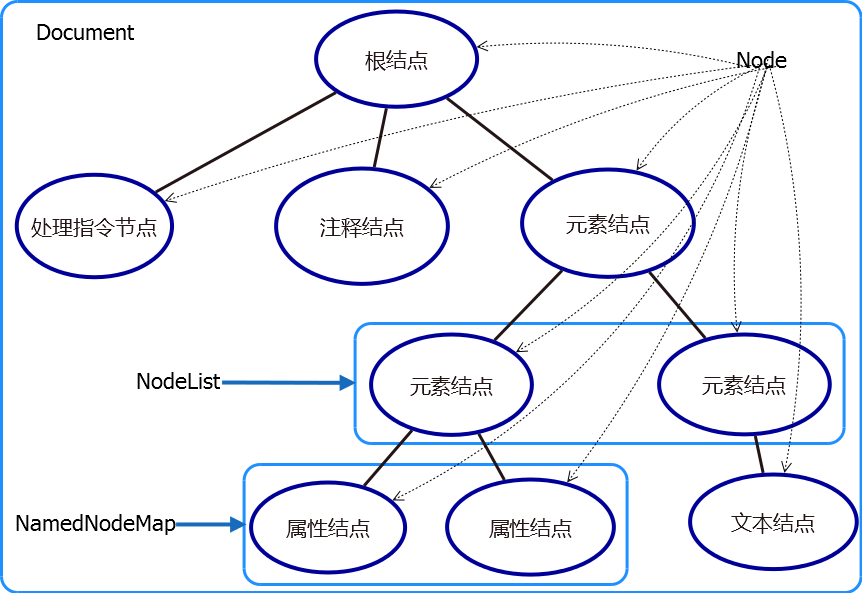
\includegraphics[width=0.9\textwidth]{figure/dom-object.png}
\end{figure}
\end{frame}



\subsection{9.3 利用Mongoose搭建DOM测试环境}

\begin{frame}[fragile]{9.3 利用Mongoose搭建DOM测试环境}
\begin{easylist} \easyitem
& Mongoose
&& 跨平台的Web服务器
& 为什么需要Web服务器
&& 访问拒绝错误
& 搭建步骤
&& 参考教材
\end{easylist}
\end{frame}


\begin{frame}[fragile]{利用浏览器访问本地搭建的Mongoose服务器}
\begin{figure}
    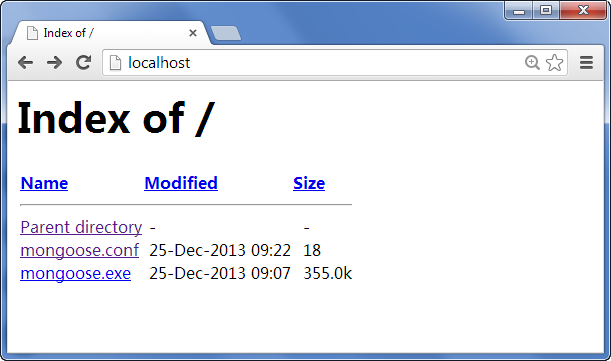
\includegraphics[width=0.9\textwidth]{figure/dom-mongoose.png}
\end{figure}
\end{frame}


\subsection{9.4 利用DOM操纵HTML}

\begin{frame}[fragile]{9.4 利用DOM操纵HTML}
\begin{easylist} \easyitem
& HTML DOM及元素定位方法
& 改变元素结点内容
& 改变属性结点内容
& 综合示例
\end{easylist}
\end{frame}


\subsubsection{9.4.1 HTML DOM及元素定位方法}
\begin{frame}[fragile, allowframebreaks]{9.4.1 HTML DOM及元素定位方法}
\begin{easylist} \easyitem
& HTML示例文档:
\begin{lstlisting}[tabsize=8, basicstyle=\small\tt, language=HTML]
<html>
    <head>
        <title>HTML DOM Example</title>
        <meta http-equiv="Content-Type" content="text/html;charset=utf-8" />
        <script type="text/javascript" src="jquery.js"></script>
    </head>
    <body id="main">
        <h1 id="headline">心情选择</h1>
        <div id="content">
            <span>今天的心情是:</span>
            <label for="happy_mood">开心</label>
            <input id="happy_mood" type="radio" name="mood" value="happy"/>
            <label for="bad_mood">心情不好</label>
            <input id="bad_mood" type="radio" name="mood" value="bad"/>
        </div>
    </body>
</html>
\end{lstlisting}
& HTML文档对于的HTML DOM树:
\begin{figure}
    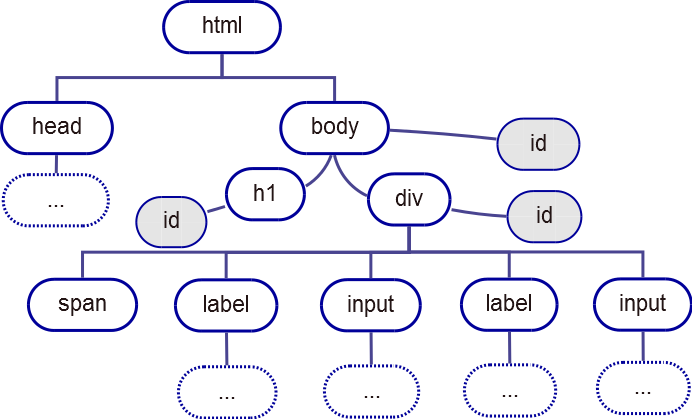
\includegraphics[width=0.75\textwidth]{figure/dom-html-tree.png}
\end{figure}
\end{easylist}
\end{frame}


\begin{frame}[fragile]{定位方法}
\begin{easylist} \easyitem
& getElementById方法
\begin{lstlisting}[tabsize=8, basicstyle=\small\tt, language=JavaScript, numbers=none]
document.getElementById("content");
\end{lstlisting}
& getElementsByName方法
\begin{lstlisting}[tabsize=8, basicstyle=\small\tt, language=JavaScript, numbers=none]
document.getElementsByTagName(“mood”);
\end{lstlisting}
& getElementsByTagName方法
\begin{lstlisting}[tabsize=8, basicstyle=\small\tt, language=JavaScript, numbers=none]
document.getElementsByTagName("h1");
\end{lstlisting}
& jQuery选择方法
\begin{lstlisting}[tabsize=8, basicstyle=\small\tt, language=JavaScript]
$('#content'); //选择id为content的元素
$('input[name="mood"]');  //选择名称为mood的所有input元素
$('h1');  //选择标签名称为h1的所有元素
\end{lstlisting}
\end{easylist}
\end{frame}



\subsubsection{9.4.2 改变元素结点内容}
\begin{frame}[fragile]{9.4.2 改变元素结点内容}
\begin{easylist} \easyitem
& innerText
\begin{lstlisting}[tabsize=8, basicstyle=\small\tt, language=JavaScript]
var headline = document.getElementById("headline");
headline.innerText = '天天好心情';
\end{lstlisting}
& innerHTML
\begin{lstlisting}[tabsize=8, basicstyle=\small\tt, language=JavaScript]
var headline = document.getElementById("headline");
headline.innerHTML = '<font color="red">天天好心情</font>';
\end{lstlisting}
& jQuery方式
\begin{lstlisting}[tabsize=8, basicstyle=\small\tt, language=JavaScript]
$('#headline').text('天天好心情');
$('#headline').html('<font color="red">天天好心情</font>');
\end{lstlisting}
\end{easylist}
\end{frame}


\subsubsection{9.4.3 改变属性结点内容}
\begin{frame}[fragile]{9.4.3 改变属性结点内容}
\begin{easylist} \easyitem
& 设置属性
&& getAttribute()
& 获取属性
&& getAttribute()
\begin{lstlisting}[tabsize=8, basicstyle=\small\tt, language=JavaScript]
var headline = document.getElementById("headline");
headline.setAttribute('style', 'color:red;');
headline.getAttribute('style');
\end{lstlisting}
& jQuery方式
\begin{lstlisting}[tabsize=8, basicstyle=\small\tt, language=JavaScript]
$('#headline').attr('style','color:red;');
$('#headline').attr('style');
\end{lstlisting}
\end{easylist}
\end{frame}


\subsubsection{9.4.4 结点的创建与删除}
\begin{frame}[fragile, allowframebreaks]{9.4.4 结点的创建与删除}
\begin{easylist} \easyitem
& 创建元素结点
&& createElement( )
& 把新创建的结点附加到特定结点内
&& appendChild( )
\begin{lstlisting}[tabsize=8, basicstyle=\small\tt, language=JavaScript]
var button = document.createElement("input");
button.setAttribute('id', 'guess_button');
button.setAttribute('type', 'button');
button.setAttribute('value', 'Guess');
var container = document.getElementById('content');
container.appendChild(button);
\end{lstlisting}
& 创建一个文本结点
&& createTextNode( )
\begin{lstlisting}[tabsize=8, basicstyle=\small\tt, language=JavaScript]
var textNode = document.createTextNode('静以修身');
container.appendChild(textNode);
\end{lstlisting}
& 删除结点
&& removeChild( )
\begin{lstlisting}[tabsize=8, basicstyle=\small\tt, language=JavaScript]
container.removeChild(textNode);
\end{lstlisting}
\end{easylist}
\end{frame}



\subsubsection{9.4.5 示例}
\begin{frame}[fragile, allowframebreaks]{9.4.5 示例}
\begin{easylist} \easyitem
& 代码清单
\begin{lstlisting}[tabsize=8, basicstyle=\small\tt, language=HTML]
<html>
    <head>
        <title>HTML DOM Example</title>
        <meta http-equiv="Content-Type" content="text/html;charset=utf-8" />
        <script type="text/javascript" src="jquery.js"></script>
        <script type="text/javascript">
            $(document).ready(function(){
                var headline = document.getElementById("headline");
                
                headline.innerText = '天天好心情'; 
                headline.innerHTML = '<font color="red">天天好心情</font>'; 
            
                $('#headline').text('天天好心情'); 
                $('#headline').html('<font color="red">天天好心情</font>'); 
                
                headline.setAttribute('style', 'color:red;'); 
                console.info(headline.getAttribute('style')); //获取h1的style属性值
                
                $('#headline').attr('style','color:red;'); 
                console.info($('#headline').attr('style')); //获取h1的style属性值
                
                var button = document.createElement("input");
                button.setAttribute('id', 'guess_button'); 
                button.setAttribute('type', 'button'); 
                button.setAttribute('value', 'Guess'); 
                var container = document.getElementById('content'); 
                container.appendChild(button);  //把创建的button结点附加到id为content的元素下
                
                var textNode = document.createTextNode('静以修身'); 
                container.appendChild(textNode); 
                
                container.removeChild(button); //删除结点
            });
        </script>
    </head>
    <body id="main">
        <h1 id="headline">心情选择</h1>
        <div id="content">
            <span>今天的心情是:</span>
            <label for="happy_mood">开心</label>
            <input id="happy_mood" type="radio" name="mood" value="happy"/>
            <label for="bad_mood">心情不好</label>
            <input id="bad_mood" type="radio" name="mood" value="bad"/>
        </div>
    </body>
</html>
\end{lstlisting}
& 显示效果
\begin{figure}
    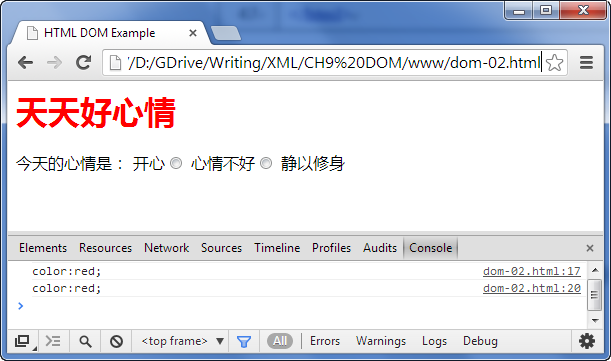
\includegraphics[width=0.75\textwidth]{figure/dom-html-display.png}
\end{figure}
\end{easylist}
\end{frame}



\subsection{9.5 利用DOM操纵XML}

\begin{frame}[fragile]{9.5 利用DOM操纵XML}
\begin{easylist} \easyitem
& 加载XML文档
& 结点访问方法
& 结点定位属性
& 结点常用属性
& 结点常用方法
& 示例
\end{easylist}
\end{frame}

\begin{frame}[fragile, allowframebreaks]{示例XML文档:books.xml}
\begin{lstlisting}[tabsize=8, basicstyle=\small\tt, language=XML]
<?xml version="1.0"?>
<books>
    <book isbn="978-1449319793" id=”b1”>
        <title lang="EN">Python for Data Analysis</title>
        <price currency="dollar">25.40</price>
        <authors>
            <author>Wes McKinney</author>
        </authors>
        <press> O'Reilly Media</press>
        <pages>470</pages>
        <description>Python for Data Analysis is concerned with the nuts…</description>
        <cover>book-python.jpg</cover>
    </book>
    <book isbn="978-7-115-28282-8" id=”b2”>
        <title lang="CHN">数学之美</title>
        <price>45.00</price>
        <authors>
            <author>吴军</author>
        </authors>
        <press>人民邮电出版社</press>
        <pages>304</pages>
        <description>读了“数学之美”,才发现大学时学的数学知识…</description>
        <cover>book-math.jpg</cover>
    </book>
</books>
\end{lstlisting}
\end{frame}


\subsection{9.5.1 加载XML文档}
\begin{frame}[fragile, allowframebreaks]{9.5.1 加载XML文档}
\begin{easylist} \easyitem
& XMLHttpRequest
&& IE7+、Firefox、Chrome、Safari以及Opera
&& 老版本的浏览器可能不支持
& 自定义的加载XML文档函数
\begin{lstlisting}[tabsize=8, basicstyle=\small\tt, language=JavaScript]
function loadXml(xmlFile) {
    var xhttp = new XMLHttpRequest();
    xhttp.open("GET", xmlFile, false); 
    xhttp.send();
    return xhttp.responseXML;
}
\end{lstlisting}
& XMLHttpRequest的open()
\begin{lstlisting}[tabsize=8, basicstyle=\small\tt, language=JavaScript, numbers=none]
void open(string method, string URL, boolean asynch, string username, string password);
\end{lstlisting}
&& method
&&& 向服务器发送请求的方式
&&& 可以为GET或POST
&& URL
&&& 所调用的服务器资源的URL
&& asynch
&&& 布尔值,说明调用时是异步方式还是同步方式
&&& 默认为true,即异步调用方式
&& username和password
&&& 在必要时指定访问资源所需要的用户名和口令
& XMLHttpRequest的send()
\begin{lstlisting}[tabsize=8, basicstyle=\small\tt, language=JavaScript, numbers=none]
void send(content);
\end{lstlisting}
&& 如open()方法中的asynch参数为true,send()方法就会立即返回
&& 否则它会等待,直到接收到响应为止
&& content是可选参数
& XMLHttpRequest的返回结果
&& responseXML 
&& responseText
\end{easylist}
\end{frame}

\begin{frame}[fragile]{利用DOMParser对象从字符串中加载XML}
\begin{lstlisting}[tabsize=8, basicstyle=\small\tt, language=JavaScript]
function loadXmlFromString(str) {
    var parser = new DOMParser();
    var xmlDoc = parser.parseFromString(str, "text/xml");
    return xmlDoc
}
\end{lstlisting}
\end{frame}


\subsection{9.5.2 结点访问方法}
\begin{frame}[fragile]{9.5.2 结点访问方法}
\begin{easylist} \easyitem
& 获取指定结点下指定标记名称的结点集合
\begin{lstlisting}[tabsize=8, basicstyle=\small\tt, language=JavaScript, numbers=none]
node.getElementsByTagName("tagname");
\end{lstlisting}
&& 返回结果为NodeList
&&& 可通过下标访问每一个结点
&&& 可通过length属性获取结点集合的大小
&&& 示例:
\begin{lstlisting}[tabsize=8, basicstyle=\small\tt, language=JavaScript]
var titleList = xmlDoc.getElementsByTagName("title");
for(var i=0; i<titleList.length; i++) {
    var titleNode = titleList[i]; 
    //其他处理
}
\end{lstlisting}
\end{easylist}
\end{frame}


\subsection{9.5.3 结点定位属性}
\begin{frame}[fragile]{9.5.3 结点定位属性}
\begin{easylist} \easyitem
& 从当前结点根据结点树关系进行访问
&& parentNode:返回当前结点的父节点。
&& childNodes:该属性用于获取当前结点的直接子结点集合,返回结果为NodeList对象,与getElementsByTagName()方法相同。
&& firstChild:返回当前结点的第一个孩子结点。
&& lastChild:返回当前结点的最后一个孩子结点。
&& nextSibling:返回当前结点的下一个兄弟结点。
&& previousSibling:返回当前结点的上一个兄弟结点。
\end{easylist}
\end{frame}

\begin{frame}[fragile]{示例}
\begin{lstlisting}[tabsize=8, basicstyle=\small\tt, language=JavaScript]
var firstBookNode = xmlDoc.getElementsByTagName('book')[0];
for(var node = firstBookNode.firstChild; 
        node!=null; 
        node = node.nextSibling) {
    console.info(node);
    if(node==firstBookNode.lastChild) break;
}
\end{lstlisting}
\end{frame}


\subsection{9.5.4 结点常用属性}
\begin{frame}[fragile]{9.5.4 结点常用属性}
\begin{easylist} \easyitem
& nodeName
& nodeValue
& nodeType
& attributes
\end{easylist}
\end{frame}

\begin{frame}[fragile]{nodeName}
\begin{easylist} \easyitem
& 元素结点的nodeName与标签名相同
& 属性结点的nodeName是属性的名称
& 文本结点的nodeName永远是“\#text”
& 文档结点的nodeName永远是“\#document”
\end{easylist}
\end{frame}

\begin{frame}[fragile]{nodeValue}
\begin{easylist} \easyitem
& 元素结点的nodeValue是undefined
& 文本结点的nodeValue是文本自身
& 属性结点的nodeValue是属性的值
\end{easylist}
\end{frame}

\begin{frame}[fragile]{nodeType}
\begin{table}[!hbp] 
\begin{tabular}{l|l|l}
\Xhline{1.3pt}
结点类型 & 常量字符串 & 数值表示结果\\ \Xhline{1.3pt}
元素结点 & ELEMENT\_NODE & 1 \\ \hline
属性结点 & ATTRIBUTE\_NODE & 2 \\ \hline
文本结点 & TEXT\_NODE & 3 \\ \hline
CDATA块结点 & CDATA\_SECTION\_NODE & 4 \\ \hline
实体引用结点 & ENTITY\_REFERENCE\_NODE & 5 \\ \hline
实体结点 & ENTITY\_NODE & 6 \\ \hline
处理指令结点 & PROCESSING\_INSTRUCTION\_NODE & 7 \\ \hline
注释结点 & COMMENT\_NODE & 8 \\ \hline
文档结点 & DOCUMENT\_NODE & 9 \\ \hline
文档类型结点 & DOCUMENT\_TYPE\_NODE & 10 \\ \hline
文档片段结点 & DOCUMENT\_FRAGMENT\_NODE & 11 \\ \hline
NOTATION结点 & NOTATION\_NODE & 12 \\ \hline
\end{tabular}
\end{table}
\end{frame}

\begin{frame}[fragile]{attributes}
\begin{easylist} \easyitem
& 如果当前结点是元素类型的结点,attributes包含了当前元素的所有属性信息,否则为null
& attributes类型:NamedNodeMap
&& 无序结点集合
\end{easylist}
\end{frame}



\subsection{9.5.5 结点常用方法}
\begin{frame}[fragile]{9.5.5 结点常用方法}
\begin{easylist} \easyitem
& appendChild
& cloneNode
& hasChildNodes
& createElement
& insertBefore
& removeChild
& replaceChild
\end{easylist}
\end{frame}


\subsection{9.5.6 完整示例}
\begin{frame}[fragile, allowframebreaks]{9.5.6 完整示例}
\begin{easylist} \easyitem
& 在浏览器中显示"books.xml"的主要文档结构
& dom-tree.js
\begin{lstlisting}[tabsize=8, basicstyle=\small\tt, language=JavaScript]
function loadXmlFromFile(xmlFile) {
    var xhttp = new XMLHttpRequest();
    xhttp.open("GET", xmlFile, false); 
    xhttp.send();
    return xhttp.responseXML; 
}

var buffer = '';
$(document).ready(function () {
    var xmlDoc = loadXmlFromFile('books.xml'); //加载xml文档
    showTree(xmlDoc, 0);    //调用showTree()函数,输出结点树
    $('#main').html(buffer); //替换网页内容
});

function showTree(node, depth) {
    //输出当前node结点的信息
    writeNode(node, depth); 
    
    //循环输出当前结点的子结点信息
    var child = node.firstChild; 
    for(var child=node.firstChild;child!=null; child = child.nextSibling){ 
        showTree(child, depth + 4); 
        if(child==node.lastChild) break; 
    }
}

function writeNode(node, depth){
    if(node.nodeType==3){ 
        //忽略文本结点
        return; 
    } else if(node.nodeType==9){ //文档结点
        //处理文档结点
        buffer = node.nodeName; 
    } else if(node.nodeType == 1) {
        //处理元素结点
        buffer = buffer + '<br/>'; 
        for(var d=0; d<depth; d++) 
            buffer = buffer + '+'; 
            
        buffer = buffer + node.nodeName; 
        
        //处理元素的属性
        var attributes = node.attributes; 
        if(attributes.length > 0) {
            buffer = buffer + '['; 
            for(var i=0; i<attributes.length; i++) {
                if(i>0) buffer = buffer + ', '; 
                var att = attributes[i]; 
                buffer = buffer + att.nodeName + '=' + att.nodeValue; 
            }
            buffer = buffer + '] ';
        }
    }
}
\end{lstlisting}
& dom-tree.html
\begin{lstlisting}[tabsize=8, basicstyle=\small\tt, language=HTML]
<html>
    <head>
        <title>HTML DOM Node Test</title>
        <meta http-equiv="Content-Type" content="text/html;charset=utf-8" />
        <script type="text/javascript" src="jquery.js"></script>
        <!-- 引用dom-tree.js, 调用编写的脚本文件 -->
        <script type="text/javascript" src="dom-tree.js"></script>
    </head>
    <body id="main"></body>
</html>
\end{lstlisting}
& 在浏览器中的运行结果
\begin{figure}
    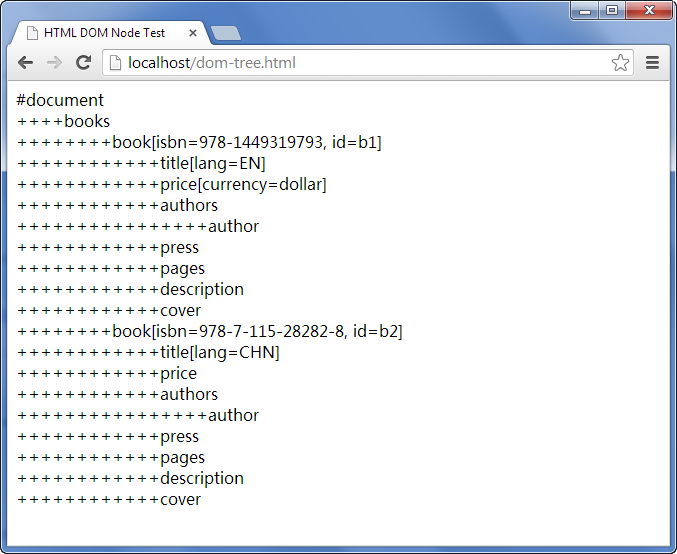
\includegraphics[width=0.75\textwidth]{figure/dom-tree.png}
\end{figure}
\end{easylist}
\end{frame}



\begin{frame}
\begin{center}
    \Huge END
\end{center}
\begin{figure}
    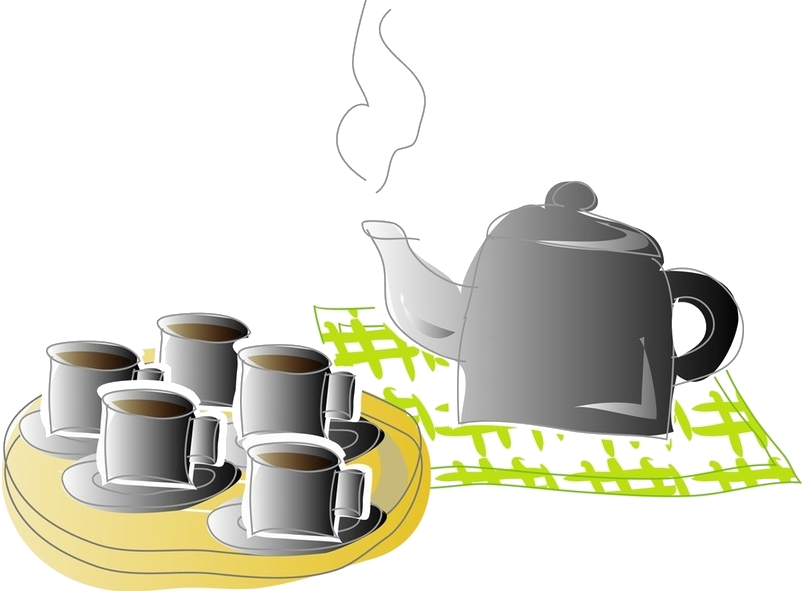
\includegraphics[width=0.75\textwidth]{figure/relax.png}
\end{figure}
\end{frame}

%\section{ APP}

\begin{frame}[fragile]{CH10 XML的应用与挑战——SVG \& JSON}
\begin{figure}
    \includegraphics[width=0.5\textwidth]{figure/app.png}
\end{figure}
\end{frame}

\begin{frame}[fragile]{本章学习目标}
\begin{easylist} \easyitem
& 了解SVG的特点
& 能够基于SVG进行简单的图形表示
& 了解d3.js的功能特点
& 掌握JSON的数据结构和类型
& 能够通过JavaScript解析JSON字符串

\end{easylist}
\end{frame}

\begin{frame}[fragile]{目录}
\begin{easylist} \easyitem
& 概述
& SVG
&& SVG的基本形状
&& SVG的样式设置
&& SVG的层与重叠
&& SVG的透明度
&& 基于SVG的d3.js图形绘制库
& JSON
&& JSON的数据结构
&& JSON的值类型
&& JSON与XML的对比
&& 利用JavaScript解析JSON
\end{easylist}
\end{frame}


\subsection{10.1 概述}

\begin{frame}[fragile]{10.1 概述}
\begin{easylist} \easyitem
& SVG
&& 可缩放矢量图形(Scalable Vector Graphics)
&& 1999年推出
& JSON
&& JavaScript Object Notation
&& 尤其适合作为数据传输格式
& SVG、JSON、XML是Web技术体系的重要组成部分
\end{easylist}
\end{frame}

\begin{frame}[fragile]{PNG与SVG文件缩放对比}
\begin{figure}
    \includegraphics[width=0.85\textwidth]{figure/app-svg-vs-png.png}
\end{figure}
\end{frame}


\subsection{10.2 SVG}

\begin{frame}[fragile]{10.2 SVG}
\begin{easylist} \easyitem
& 通过XML定义线段、圆形、矩形等形状
\begin{lstlisting}[tabsize=8, basicstyle=\small\tt, language=XML]
<svg xmlns="http://www.w3.org/2000/svg" width="50" height="50">
    <circle cx="25" cy="25" r="22" fill="blue" stroke="gray" stroke-width="2"/>
</svg>
\end{lstlisting}
\end{easylist}
\end{frame}


\begin{frame}[fragile, allowframebreaks]{SVG示例}
\begin{lstlisting}[tabsize=8, basicstyle=\small\tt, language=HTML, caption="circle.html"]
<!DOCTYPE html>
<html>
    <head>
        <title>SVG Circle</title>
    </head>
    <body>
        <svg width="50" height="50">
            <circle cx="25" cy="25" r="22" fill="blue" stroke="gray" stroke-width="2"/>
        </svg>
    </body>
</html>
\end{lstlisting}

\begin{figure}
    \includegraphics[width=0.2\textwidth]{figure/app-circle.png}
\end{figure}
\end{frame}


\begin{frame}[fragile]{Linux Imagte Viewer}
\begin{figure}
    \includegraphics[width=0.4\textwidth]{figure/app-svg-viewer.png}
\end{figure}
\begin{figure}
    \includegraphics[width=0.4\textwidth]{figure/app-svg-viewer2.png}
\end{figure}
\end{frame}


\subsubsection{10.2.1 SVG的基本形状}
\begin{frame}[fragile, allowframebreaks]{10.2.1 SVG的基本形状}
\begin{easylist} \easyitem
& 基本形状
&& 矩形:rect
&& 圆形:circlue
&& 椭圆:Ellipse
&& 线条:line
&& 文本:Text

& 坐标系
\begin{figure}
    \includegraphics[width=0.9\textwidth]{figure/svg-coordinates.png}
\end{figure}
\end{easylist}
\end{frame}


\begin{frame}[fragile, allowframebreaks]{绘制矩形}
\begin{easylist} \easyitem
& 代码
\begin{lstlisting}[tabsize=8, basicstyle=\small\tt, language=XML, numbers=none]
<rect x="0" y="0" width="300" height="50"/>
\end{lstlisting}
& 效果
\begin{figure}
    \includegraphics[width=0.5\textwidth]{figure/svg-rect.png}
\end{figure}

\newpage
& 代码
\begin{lstlisting}[tabsize=8, basicstyle=\small\tt, language=XML, numbers=none]
<rect x="0" y="0" width="300" height="50" rx="15" ry="15"/>
\end{lstlisting}
& 效果
\begin{figure}
    \includegraphics[width=0.5\textwidth]{figure/svg-rect2.png}
\end{figure}
\end{easylist}
\end{frame}


\begin{frame}[fragile, allowframebreaks]{绘制椭圆}
\begin{easylist} \easyitem
& 代码
\begin{lstlisting}[tabsize=8, basicstyle=\small\tt, language=XML, numbers=none]
<ellipse cx="250" cy="25" rx="50" ry="25"/>
\end{lstlisting}
& 效果
\begin{figure}
    \includegraphics[width=0.2\textwidth]{figure/svg-ellipse.png}
\end{figure}
\end{easylist}
\end{frame}


\begin{frame}[fragile, allowframebreaks]{绘制线条}
\begin{easylist} \easyitem
& 代码
\begin{lstlisting}[tabsize=8, basicstyle=\small\tt, language=XML, numbers=none]
<line x1="0" y1="0" x2="350" y2="50" stroke="black"/>
\end{lstlisting}
& 效果
\begin{figure}
    \includegraphics[width=0.9\textwidth]{figure/svg-line.png}
\end{figure}
\end{easylist}
\end{frame}

\begin{frame}[fragile, allowframebreaks]{绘制文本}
\begin{easylist} \easyitem
& 代码
\begin{lstlisting}[tabsize=8, basicstyle=\small\tt, language=XML, numbers=none]
<text x="250" y="25" font-family="华文隶书" font-size="30" fill="navy">可缩放矢量图形</text>
\end{lstlisting}
& 效果
\begin{figure}
    \includegraphics[width=0.5\textwidth]{figure/svg-text.png}
\end{figure}
\end{easylist}
\end{frame}



\subsubsection{10.2.2 SVG的样式设置}
\begin{frame}[fragile]{10.2.2 SVG的样式设置}
\begin{easylist} \easyitem
& 默认样式为黑色填充、无stroke
& fill
&& 填充色,取值为有效的CSS颜色值,如颜色名称red、blue,或者RGB、RGBA值。
& stroke
&& 线条的颜色值
& stroke-width
&& 数值,通常采用像素单位
& opacity
&& 透明度,介于0.0到1.0之间的数值,0.0表示完全透明,1.0表示完全不透明
& font-family、font-size
&& 应用于文本
\end{easylist}
\end{frame}


\begin{frame}[fragile]{样式关联方式}
\begin{easylist} \easyitem
& 内联方式
\begin{lstlisting}[tabsize=8, basicstyle=\small\tt, language=XML, numbers=none]
<circle cx="50" cy="50" r="30" fill="yellow" stroke="orange" stroke-width="10"/>
\end{lstlisting}
& CSS样式属性关联方式
\begin{lstlisting}[tabsize=8, basicstyle=\small\tt, language=XML, numbers=none]
<circle cx="50" cy="50" r="30" class="pumpkin"/>
\end{lstlisting}
&& 需要设置pumpkin样式
& 效果
\begin{figure}
    \includegraphics[width=0.1\textwidth]{figure/svg-pumpkin.png}
\end{figure}
\end{easylist}
\end{frame}


\begin{frame}[fragile, allowframebreaks]{示例网页}
\begin{lstlisting}[tabsize=8, basicstyle=\small\tt, language=HTML]
<!DOCTYPE html>
<html>
    <head>
        <title>SVG Style</title>
        <style>
            .pumpkin {
                fill: yellow;
                stroke: orange;
                stroke-width: 10;
            }
        </style>
    </head>
    <body>
        <svg width="500px" height="200px">
            <circle cx="50" cy="50" r="30" class="pumpkin"/>
        </svg>
    </body>
</html>
\end{lstlisting}
\end{frame}


\subsubsection{10.2.3 SVG的层与重叠}
\begin{frame}[fragile]{10.2.3 SVG的层与重叠}
\begin{easylist} \easyitem
& 根据绘制的先后顺序予以覆盖
\begin{lstlisting}[tabsize=8, basicstyle=\small\tt, language=XML]
<rect x="0" y="0" width="50" height="50" fill="red"/>
<rect x="25" y="15" width="50" height="50" fill="green"/>
<rect x="50" y="30" width="50" height="50" fill="blue"/>
<rect x="75" y="45" width="50" height="50" fill="gray"/>
<rect x="100" y="60" width="50" height="50" fill="navy"/>
\end{lstlisting}

\begin{figure}
    \includegraphics[width=0.4\textwidth]{figure/svg-overlapping.png}
\end{figure}
\end{easylist}
\end{frame}


\subsubsection{10.2.4 SVG的透明度}
\begin{frame}[fragile]{10.2.4 SVG的透明度}
\begin{easylist} \easyitem
& 使用带alpha的RGB颜色函数rgba()
& 设置opacity属性值。
\end{easylist}
\end{frame}


\begin{frame}[fragile, allowframebreaks]{rgba()}
\begin{easylist} \easyitem
& 代码:
\begin{lstlisting}[tabsize=8, basicstyle=\small\tt, language=XML]
<circle cx="50" cy="50" r="40" fill="rgba(0, 150, 150, 1.0)"/>
<circle cx="100" cy="50" r="40" fill="rgba(0, 0, 255, 0.75)"/>
<circle cx="150" cy="50" r="40" fill="rgba(0, 255, 0, 0.5)"/>
<circle cx="200" cy="50" r="40" fill="rgba(255, 255, 0, 0.6)"/>
<circle cx="250" cy="50" r="40" fill="rgba(255, 0, 0, 0.3)"/>
\end{lstlisting}
& 显示效果:
\begin{figure}
    \includegraphics[width=0.4\textwidth]{figure/svg-rgba.png}
\end{figure}

\newpage
& 代码:
\begin{lstlisting}[tabsize=8, basicstyle=\small\tt, language=XML]
<circle cx="50" cy="50" r="40" fill="rgba(0, 150, 150, 1.0)" 
        stroke="rgba(0, 255, 0, 0.25)" stroke-width="10"/>
<circle cx="100" cy="50" r="40" fill="rgba(0, 0, 255, 0.75)" 
        stroke="rgba(0, 0, 255, 0.25)" stroke-width="10"/>
<circle cx="150" cy="50" r="40" fill="rgba(0, 255, 0, 0.5)" 
        stroke="rgba(0, 0, 255, 0.25)" stroke-width="10"/>
<circle cx="200" cy="50" r="40" fill="rgba(255, 255, 0, 0.6)" 
        stroke="rgba(255, 0, 0, 0.25)" stroke-width="10"/>
<circle cx="250" cy="50" r="40" fill="rgba(255, 0, 0, 0.3)" 
        stroke="rgba(55, 255, 0, 0.25)" stroke-width="10"/>
\end{lstlisting}
& 显示效果:
\begin{figure}
    \includegraphics[width=0.4\textwidth]{figure/svg-rgba2.png}
\end{figure}
\end{easylist}
\end{frame}


\begin{frame}[fragile, allowframebreaks]{opacity}
\begin{easylist} \easyitem
& opacity设置为1.0表示完全不透明,为默认值
\begin{lstlisting}[tabsize=8, basicstyle=\small\tt, language=XML]
<circle cx="50" cy="50" r="40" fill="green" stroke="orange" stroke-width="10" opacity="1.0"/>
<circle cx="120" cy="50" r="40" fill="yellow" stroke="red" stroke-width="10"/>
<circle cx="190" cy="50" r="40" fill="orange" stroke="blue" stroke-width="10"/>
\end{lstlisting}
& 显示效果:
\begin{figure}
    \includegraphics[width=0.4\textwidth]{figure/svg-opacity.png}
\end{figure}

\newpage
& 代码:
\begin{lstlisting}[tabsize=8, basicstyle=\small\tt, language=XML]
<circle cx="50" cy="50" r="40" fill="green" stroke="orange" stroke-width="10" opacity="0.5"/>
<circle cx="120" cy="50" r="40" fill="yellow" stroke="red" stroke-width="10" opacity="0.3"/>
<circle cx="190" cy="50" r="40" fill="orange" stroke="blue" stroke-width="10" opacity="0.1"/>
\end{lstlisting}
& 显示效果:
\begin{figure}
    \includegraphics[width=0.4\textwidth]{figure/svg-opacity2.png}
\end{figure}
\end{easylist}
\end{frame}


\begin{frame}[fragile, allowframebreaks]{同时设置rgba与opacity}
\begin{easylist} \easyitem
& 代码:
\begin{lstlisting}[tabsize=8, basicstyle=\small\tt, language=XML]
<circle cx="50" cy="50" r="40" fill="green" stroke="orange" stroke-width="10" opacity="0.5"/>
<circle cx="120" cy="50" r="40" fill="yellow" 
        stroke="rgba(255, 0, 0, 0.5)" stroke-width="10" opacity="0.3"/>
<circle cx="190" cy="50" r="40" fill="orange" stroke="blue" stroke-width="10" opacity="0.1"/>
\end{lstlisting}
& 显示效果:
\begin{figure}
    \includegraphics[width=0.4\textwidth]{figure/svg-opacity3.png}
\end{figure}
\end{easylist}
\end{frame}



\subsubsection{10.2.5 d3.js}
\begin{frame}[fragile]{10.2.5 d3.js}
\begin{easylist} \easyitem
& d3
&& Data-Driven Documents的缩写
&& Data表示用户提供的数据
&& Documents代表可以被浏览器解析呈现的文档,
&& 支持SVG
\end{easylist}
\end{frame}

\begin{frame}[fragile, allowframebreaks]{效果图}
\begin{figure}
    \includegraphics[width=0.5\textwidth]{figure/d3.demo1.png}
\end{figure}

\newpage
\begin{figure}
    \includegraphics[width=0.5\textwidth]{figure/d3.demo2.png}
\end{figure}
\newpage
\begin{figure}
    \includegraphics[width=0.5\textwidth]{figure/d3.demo3.png}
\end{figure}
\newpage
\begin{figure}
    \includegraphics[width=0.5\textwidth]{figure/d3.demo4.png}
\end{figure}
\end{frame}


\begin{frame}[fragile]{如何引用d3.js进行测试}
\begin{easylist} \easyitem
& 下载最新版本的d3.js
& 在网页中引用d3.js
& 在Web Server中测试(可选)
\end{easylist}
\end{frame}


\begin{frame}[fragile, allowframebreaks]{基于d3.js绘制SVG图形}
\begin{easylist} \easyitem
& 创建svg元素,设置属性
\begin{lstlisting}[tabsize=8, basicstyle=\small\tt, language=JavaScript,numbers=none]
var svg = d3.select("body").append("svg");
svg.attr("width", 500);
svg.attr("height", 200);
\end{lstlisting}

& 采用链式语法改写
\begin{lstlisting}[tabsize=8, basicstyle=\small\tt, language=JavaScript,numbers=none]
var svg = d3.select("body") 
        .append("svg")
        .attr("width", 500)
        .attr("height", 200);
\end{lstlisting}

& 继续增加若干圆形
\begin{lstlisting}[tabsize=8, basicstyle=\small\tt, language=JavaScript,numbers=none]
var dataset = [ 20, 15, 10, 5, 10, 15, 20 ];
var circles = svg.selectAll("circle")
        .data(dataset)
        .enter()
        .append("circle");
\end{lstlisting}

& 继续指定图形的位置和大小
\begin{lstlisting}[tabsize=8, basicstyle=\small\tt, language=JavaScript,numbers=none]
circles.attr("cx", function(d, i) {
            return (i * 50) + 25;
          })
        .attr("cy", 50)
        .attr("r", function(d) {
            return d;
          });
\end{lstlisting}
&& 代码中d表示传入函数的绑定数据,i代表图形顺序编号,起始编号为0
& 显示效果
\begin{figure}
    \includegraphics[width=0.5\textwidth]{figure/d3.circles.png}
\end{figure}
& 继续指定圆的样式
\begin{lstlisting}[tabsize=8, basicstyle=\small\tt, language=JavaScript,numbers=none]
.attr("fill", "orange")
.attr("stroke", "red")
.attr("stroke-width", function(d, i) {
    return d/3;
});
\end{lstlisting}
& 显示效果
\begin{figure}
    \includegraphics[width=0.5\textwidth]{figure/d3.circles2.png}
\end{figure}
\end{easylist}
\end{frame}




\begin{frame}[fragile, allowframebreaks]{代码清单}
\begin{lstlisting}[tabsize=8, basicstyle=\small\tt, language=HTML]
<!DOCTYPE html>
<html>
    <head>
        <meta charset="utf-8" />
        <title>D3 Circles</title>
        <script type="text/javascript" src="d3/d3.v3.js"></script>
    </head>
    <body>
        <script type="text/javascript">
            var svg = d3.select("body")
                    .append("svg")
                    .attr("width", 500) 
                    .attr("height", 200); 
            var dataset = [20, 15, 10, 5, 10, 15, 20]; 
            var circles = svg.selectAll("circle")
                              .data(dataset) 
                              .enter()
                              .append("circle");

            circles.attr("cx", function(d, i) {
                return (i * 50) + 25; 
            })
            .attr("cy", 50) 
            .attr("r", function(d) {
                return d; 
            })
            .attr("fill", "orange")
            .attr("stroke", "red")
            .attr("stroke-width", function(d, i) {
                return d/3; 
            });
        </script>
    </body>
</html>
\end{lstlisting}
\end{frame}



\subsection{10.3 JSON}

\begin{frame}[fragile]{10.3 数据传输的挑战者—JSON}
\begin{easylist} \easyitem
& JSON
&& JavaScript Object Notation
&& 一种轻量级、基于文本、语言无关的数据交换格式
&& JavaScript(Standard ECMA-262)的一个子集
&& 重要贡献者:Douglas Crockford
&& 2006年7月——RFC 4627
\end{easylist}
\end{frame}


\subsubsection{10.3.1 JSON的数据结构}
\begin{frame}[fragile]{10.3.1 JSON的数据结构}
\begin{easylist} \easyitem
& 无序的键值对集合
\begin{lstlisting}[tabsize=8, basicstyle=\small\tt, language=JavaScript, numbers=none]
{ "a":1,"b":2,"c":3 }
\end{lstlisting}
& 值的有序列表
\begin{lstlisting}[tabsize=8, basicstyle=\small\tt, language=JavaScript, numbers=none]
[ 1, 2, 3, "hello world" ]
\end{lstlisting}
\end{easylist}
\end{frame}


\subsubsection{10.3.2 JSON的值类型}
\begin{frame}[fragile]{10.3.2 JSON的值类型}
\begin{easylist} \easyitem
& 符串类型
&& JSON字符串采用双引号包括所表示的字符内容,字符内容本身包含的双引号使用反斜线进行转义;
& 数值类型
& 对象类型
&& 键值对的无序集合;
& 数组类型
&& 值的有序列表;
& 布尔类型
&& true表示真、false表示假;
& 空类型null
\end{easylist}
\end{frame}

\begin{frame}[fragile, allowframebreaks]{JSON示例}
\begin{lstlisting}[tabsize=8, basicstyle=\small\tt, language=JavaScript, caption=contact.json]
{
    "name": "王某某",
    "age": 30,
    "spouse": {
        "name": "张某某",
        "age": 28
    },
    "addresses": [
        {
            "description": "工作住址",
            "street": "胜利大街9号",
            "city": "潍坊",
            "province": "山东"
        }
    ], 
    "phoneNumbers": [
        {
            "description": "办公电话",
            "number": "6666-7777"
        },
        {
            "description": "手机",
            "number": "1XX-1234-5678"
        }
    ]
}
\end{lstlisting}
\end{frame}


\subsubsection{10.3.3 JSON与XML的对比}
\begin{frame}[fragile]{10.3.3 JSON与XML的对比}
\begin{easylist} \easyitem
& XML比JSON更易于人工阅读
& XML是典型的标记语言,而JSON不是
& JSON格式简洁,文件的体积较小,有利于数据传输。
& JSON与JavaScript结合紧密,构造和解析都比较容易,而通过JavaScript解析XML,则需要借助于额外的库
\end{easylist}
\end{frame}


\begin{frame}[fragile, allowframebreaks]{contact.json对应的XML}
\begin{lstlisting}[tabsize=8, basicstyle=\small\tt, language=XML, caption=contact.xml]
<contact>
    <name>王某某</name>
    <age>30</age>
    <spouse>
        <name>张某某</name>
        <age>28</age>
    </spouse>
    <addresses>
        <address>
            <description>工作住址</description>
            <street>胜利大街9号</street>
            <city>潍坊</city>
            <province>山东</province>
        </address>
    </addresses>
    <phoneNumbers>
        <phoneNumber>
            <description>办公电话</description>
            <number>6666-7777</number>
        </phoneNumber>
        <phoneNumber>
            <description>手机</description>
            <number>1XX-1234-5678</number>
        </phoneNumber>
    </phoneNumbers>
</contact>
\end{lstlisting}
\end{frame}


\subsubsection{10.3.4 利用JavaScript解析JSON}
\begin{frame}[fragile]{10.3.4 利用JavaScript解析JSON}
\begin{easylist} \easyitem
& 浏览器内置的JSON.parse()
\begin{lstlisting}[tabsize=8, basicstyle=\small\tt, language=JavaScript, numbers=none]
JSON.parse(text [, reviver])
\end{lstlisting}
\end{easylist}
\end{frame}


\begin{frame}[fragile, allowframebreaks]{示例}
\begin{easylist} \easyitem
& 在浏览器控制台输入以下代码
\begin{lstlisting}[tabsize=8, basicstyle=\small\tt, language=JavaScript, numbers=none]
var jsontext = '{"name":"王某某", "age": 30, \
                 "phoneNumbers": ["6666-7777", "1XX-1234-5678"]}';
var contact = JSON.parse(jsontext); 
document.write(contact.name + ", " + contact.age); 
document.write("<br/>");
document.write("main phone: ");
document.write(contact.phoneNumbers[0]); 

contact2 = JSON.parse(jsontext, function(key, value){ 
    if(typeof value === 'number'){ 
        return value - 5; 
    } else {
        return value; 
    }
}); 
document.write("<br/><hr/> 指定了reviver匿名函数,转换后的年龄属性值为:");
document.write(contact2.age);
\end{lstlisting}
& 浏览器解析结果
\begin{figure}
    \includegraphics[width=0.9\textwidth]{figure/app-json.png}
\end{figure}
\end{easylist}
\end{frame}


\begin{frame}
\begin{center}
    \Huge END
\end{center}
\begin{figure}
    \includegraphics[width=0.75\textwidth]{figure/relax.png}
\end{figure}
\end{frame}


\end{document}
